\section{Úvod}

Tato bakalářská práce se bude zabývat vývojem aplikace pro tvorbu a zobrazování vstupních stránek osob, firem a jiných
institucí.
Takových aplikací existuje mnoho, nicméně žádná nekombinuje širší možnosti sdílení různých druhů informací a vyhledávání.
Proto jsem se rozhodl navrhnout a implementovat vlastní verzi v podobě responzivní webové aplikace, která bude
tyto požadavky bude splňovat.

Jednostránkové vstupní stránky jsou moderní cestou jak sdílet všechny své veřejné kontaktní a jiné údaje se
svými zákazníky.
Představují jakousi digitální rozšířenou alternativu k běžných fyzickým vizitkám, které však postrádají interaktivnost
a spoustu důležitých údajů.

Dále se práce zaměří na analýzu implementačních technologií, hlavně pak na programovací jazyky a frameworky urychlující vývoj.
Technologií v dnešní době existuje celá řada a každým dnem přibývají nové.
Pro účely této práce se technologie rozdělí na front-endové a back-endové.
Front-endové budou pomáhat tvořit responzivní a interaktivní uživatelské prostředí pro koncové uživatele.
Back-endové, naproti tomu, budou tvořit konkrétní logiku aplikace.
To zahrnuje převážně manipulaci s uživatelskými daty a jejich agregaci.
Součástí této práce bude průzkum celosvětově využívaných technologií pro vývoj webových aplikací.
V případě front-endu se bude jednat o nějaký z Javascriptových frameworků: Vue, React, Swelte nebo Angular.
V rámci back-endu se práce zaměří na programovací jazyky Java, Javascript, C\# a PHP a také na
podpůrné nástroje v podobě databázových systémů nebo souborových úložišť.

Po zvolení vhodných technologií bude následovat navržení uživatelského prostředí společně s interním
datovým modelem a strukturou aplikace.
Hlavním cílem bude tento návrh implementovat a jednotlivé řešené problémy popsat.

Konečným krokem bude spuštění aplikace v produkčním prostředí, která bude přístupná veřejnosti.

\section{Cíl práce}

V první řadě bude nezbytné zjistit jaké informace bude vhodné umožňovat uživatelům zobrazovat na jejich
vstupních stránkách a jak s těmito informacemi pracovat v aplikaci.
Dále bude následovat analýza a porovnání programovacích jazyků a frameworků, společně s jejich výhodami a nevýhodami.
Výsledný výběr bude kombinací požadavků aplikace, výhod jednotlivých technologií a osobních preferencí.
Avšak osobní preference budou hrát roli pouze v případě, kdy nebude možné rozhodnout čistě podle dat.

Implementace pak bude vycházet z návrhu datového modelu a struktury aplikace.
Jednotlivé řešené problémy budou představeny společně s jejich možnými řešeními.
Následovat bude popis výsledné implementace a důvod zvolení daného řešení.

Primárním cílem je vytvořit funkční interaktivní webovou aplikaci umožňující intuitivně svým uživatelům
tvořit, spravovat a sdílet své vstupní stránky s jinými uživateli.
Aplikace by měla také podporovat všechny využívané rozměry zařízení, aby byl zaručen přístup k aplikaci z mobilních
i desktopových zařízení s minimálním omezením pro uživatele.
Rovněž by aplikace měla být jednoduše spustitelná a udržitelně provozovatelná v produkčním prostředí.

Finálním cílem bude hotovu aplikace spustit v produkčním prostředí a stanovené požadavky otestovat.

\section{Vstupní stránky pro osoby a instituce}

Vstupní stránky pro osoby a instituce jsou prezentační jednostránkové webové stránky.
Tyto stránky slouží k představení daného subjektu/objektu koncovému uživateli, který o něm hledá základní
informace.
Kromě základních informací, stránky většinou obsahují všemožné kontaktní údaje a odkazy na sociální sítě pro
získání mnohem detailnějších informací.
Některé stránky umožňují reprezentovat i například firemní struktury nebo geografické lokace.
Dostupné druhý informací, které lze definovat na takových stránkách, ale nejsou jasně definované, spíše jsou
určeny konkrétní webovou aplikací poskytující tyto služby.

Tento typ stránek je velice vhodný pro sdílení svých osobních údajů a funguje jako takový rejstřík uživatelových
údajů a dalo by se popsat jako digitální rozšířené vizitky nejen pro firmy.

Pro tvorbu takovýchto stránek existuje nepřeberné množství webových aplikací, kde lze
tyto prezentace jednoduše tvořit a rovnou publikovat.
Ne všechny ale nabízí všechny zmíněné možnosti a je tak na uživatelovi, jakou webovou aplikaci zvolí.

Webové aplikace jsou aplikace, které běží ve webové prohlížeči koncového uživatele bez nutnosti jakékoliv instalace.
Tyto aplikace svá data ukládají do vzdáleného serveru a
uživatel tak může ke svým datům jednoduše přistupovat z jakéhokoliv zařízení během okamžiku.

\section{Existující webové aplikace}

Existuje spousta webových aplikací, které by se dali považovat za řešení popsané problematiky.
Nicméně žádná momentálně nekombinuje prvky sdílení kontaktních údajů, sociálních sítí a firemních struktur s plně
fulltextovým vyhledáváním bez nutnosti registrace nebo rušivých sociálních prvků.
Některé navíc neřeší ani ukládání cízích stránek do oblíbených s možností kategorizace či poznámek.
U většiny takových aplikací se totiž spoléhá na navigaci pomocí přímých odkazů, které si daný subjekt
vloží na své sociální sítě nebo vizitky.

Mezi současně nejznámější existující webové aplikace řešící tyto problémy, patří například následující.

	\subsection{Linktree}

	Pravděpodobně nejrozšířenější takovou aplikací v zahraničí je Linktree.
	Ta se zabývá především zobrazováním odkazů na sociální sítě a rozsáhlým přízpůsobením.
	Momentálně však neumožňuje fulltextově vyhledávat jednotlivé stránky nebo je ukládat do oblíbených.
	Není ani jistota, že jednotlivé odkazy směřují opravdu na skutečné sociální sítě, protože uživatelé si mohou ke každému
	odkazu zvolit vlastní ikony.
	Nezabývá se ani firemními hierarchiemi nebo otevírací dobou.
	Na druhou stranu, poskytuje spoustu napojení na externí aplikace, především pak ty statistické nebo e-commercové.

	\subsection{LinkedIn}

	Další významnou aplikací je LinkedIn.
	Ta však směřuje své zaměření spíše na firemní prostředí a pracovní zkušenosti uživatelů.
	Informace navíc nejsou veřejně dostupné bez registrace.
	Oproti Linktree, ale obsahuje fulltextové vyhledávání a možnost sledování ostatních uživatelů.
	Nevýhodou můžou být všudypřítomné reklamy nebo sociální prvky generující rušivé elementy.
	I přesto že se zaměřuje na firmy, není snadné dohledat firemní struktury nebo otevírací doby.

	\subsection{AllMyLinks}

	Méně známou alternativou je služba AllMyLinks.
	Ta nabízí velice podobné funkce jako Linktree - také nabízí pouze sdílení odkazů na sociální sítě.
	Stejně jako Linktree neposkytuje podporu ověřování odkazů oproti sociálním sítím, což má za následek
	nevěryhodnost odkazů a ošklivé uživatelské ikony.

	\subsection{Swopi}

	Swopi je další alternativou Linktree.
	Navíc se ale zabývá výrobou a prodejem chytrých fyzických karet a štítků pro rychlé zobrazení uživatelských profilů.
	Software je ale značně neintuitivní a neposkytuje více odkazů na jednu sociální síť.

	\subsection{Firmy.cz}

	Mezi české nepřímé alternativy by se dala zařadit i služba Firmy.cz, která se ale podobně jako LinkedIn zabývá
	spíše firmami a jejich zobrazením na mapě.
	Nabízí vyhledávání, otevírací dobu a základní kontakty, externí odkazy a firemní struktury jsou však značně omezené.
	Služba je navíc cílená pouze na české publikum.

	\subsection{Zlaté stránky}

	Obdobou Firmy.cz trpící podobnými problémy je další česká služba Zlaté stránky.

\section{Návrh vlastní aplikace}

Výsledná webová aplikace bude oproti konkurenčním řešení kombinovat více různých typů informací, aby tak pokryla
většinu požadavků soukromých osob, firem a objektů.

	\subsection{Karty}

	Základní obecnou jednotkou reprezentující takový subjekt či objekt bude karta; odvozenina z anglického překladu vizitky "business card".
	Každá karta bude jakási moderní rozšířená digitální náhrada klasické fyzické vizitky.
	Cílem je umožnit vyhledávat a sdílet informace soukromých osob, firem, událostí, produktů, míst, uměleckých děl a podobně.
	Jedinou podmínkou pro takový subjekt nebo objekt je existence alespoň jednoho údaje důležitého pro ostatní osoby.
	Tím může být kontaktní údaj, odkaz na jiné webové stránky (např.: sociální sítě), geografická lokace nebo
	firemní hierarchie.

	\subsection{Oblíbené karty}

	Uživatelé aplikace budou mít možnost takové karty, které je nějakým způsobem zajímají, uložit do svého profilu pro
	zjednodušení zpětného dohledání například kontaktních údajů.
	Kromě obyčejného uchování oblíbených karet bude možné karty pro lepší organizaci seskupovat do vlastních upravitelných
	složek a komentovat vlastními soukromými poznámkami.
	Tyto funkce umožní uživatelům komunikujícím s velkým počtem subjektů vyznat se v kontaktních údajích a poznámkách,
	například ohledně poslední komunikace nebo podrobností o daném subjektu bez nutnosti ručně takové informace spravovat v
	textových editorech nebo papírových poznámkách.

	\subsection{Viditelnost karet}

	Protože vyplnění takové karty může být zdlouhavý proces, i za předpokladu intuitivního \acr{UI}, je potřeba umožnit
	uživatelům skrýt karty do té doby, než budou připravené ke zveřejnění.
	Zároveň ale takovou rozpracovanou kartu může uživatel chtít někomu vzdáleně ukázat například pro ověření správnosti informací
	i bez zveřejňování.
	Karty tak budou moct mít dvě viditelnosti: veřejná a skrytá.
	Veřejná karta bude mít jednoduchou zapamatovatelnou \acr{URL} adresu a bude ji možné vyhledávat pomocí fulltextového vyhledávače.
	Skrytá karta nebude vyhledatelná pomocí vyhledávače, nicméně uživatelé vlastnící \ac{URL} odkaz na danou kartu budou mít přístup
	k jejímu zobrazení.
	Skrytá karta bude mít navíc možnost vygenerování náhodné \ac{URL} pro znemožnění uhádnutí \ac{URL} adresy nepovolenou osobou.

	\subsection{Karetní informace}

	Každá karta bude mít možnost zobrazovat různé informace o uživatelích.
	Definovatelné informace budou vždy dané, tj. budou mít vlastní strukturu v kódu, validaci správnosti hodnot a specializované
	\ac{UI}.
	Aby se předešlo zhoršení čitelnosti informací karet, nebude možné uživatelem definovat náhodné informace.
	Toto rozhodnutí by mělo pomoci především uživatelům nepříliš zdatným v dodržení přehlednosti většího množství
	informací za pomoci předem daného formátu zobrazení daných informací.
	Je však potřeba strukturu navrhnout dostatečně univerzálně, aby bylo možné v budoucnu implementovat další typy informací
	definovatelných na kartách.

	Momentálně podporovanými takovými informacemi budou:
	\begin{itemize}
		\item fotografie/avatar,
		\item kategorizační štítky,
		\item popisek,
		\item základní kontaktní údaje,
		\item odkazy na profily na sociálních sítí,
		\item generické odkazy na jakékoliv externí webové stránky,
		\item geografická lokace,
		\item hlavní otevírací doba,
		\item kanceláře, pobočky.
	\end{itemize}

	Pro rychlé vizuální rozpoznání karty bude mít autor k dispozici možnost nahrát vlastní fotografii nebo avatar s logem.
	Fotografie nebo avatar dokáže dostatečně odlišit jednotlivé karty bez nutnosti čtení názvu nebo popisku ke zjištění o
	jakou kartu se vlastně jedná.

	\paragraph{Kategorizační štítky}

	Kategorizační štítky budou sloužit pro globální kategorizaci karet pro úvodní povědomí uživatele, o jakou kartu se jedná
	a hlavně pro vyhledání karet ve stejné kategorii.
	To se může hodit pro seskupení například osob s určitým povoláním nebo vyznávaným životním stylem.
	Konkrétní využití je však na konkrétních uživatelích, definovat nemusí žádný nebo i několik.

	\paragraph{Popisek}

	Popisek bude sloužit především pro stručnou definici obsahu karty, tedy co daná karta reprezentuje.
	Předpokládá se proto, že popisek karty bude zodpovídat některé z následujících otázek?
	\begin{itemize}
		\item Je to osoba, firma, událost, dílo nebo předmět?
		\item Čím se daný subjekt či objekt zabývá v profesní nebo soukromé sféře?
		\item Proč je daný subjekt či objekt zajímavý?
	\end{itemize}
	Popisek bude mít omezenou velikost a nebude povinný, nicméně silně doporučovaný.

	\paragraph{Základní kontaktní údaje}

	Základními kontaktními údaji se v případě těchto karet rozumí: telefonní číslo, hlavní emailová adresa, webové
	stránky a \acr{IČO}.
	Uživatel si pak vybere jaké z těchto údajů bude chtít zveřejnit a jaké nikoliv.

	\paragraph{Odkazy na profily na sociálních sítích}

	Pro většiny karet, zejména pak pro karty reprezentující soukromé osoby, budou nejdůležitější odkazy na sociální sítě.
	Pro jednoduché rozlišení mezi jednotlivými sítěmi a poskytnutí koncovým uživatelům jistotu, že daný odkaz skutečně
	směřuje na ověřenou doménu, bude mít systém předdefinované podporované sociální sítě.
	Každá taková definice bude jakási šablona pro výsledné odkazy na sociální sítě a bude obsahovat oficiální název,
	dále pak názvy podle kterých bude možné síť vyhledat, ikonu, šablony validních \ac{URL} adres a kategorie.
	Uživatel tedy bude moct při tvorbě karty vybrat ručně ze seznamu konkrétní síť nebo nechat aplikaci nalézt správnou
	síť podle vložené \ac{URL} adresy.

	Šablony sítí budou kategorizované a bude možné je pro jednodušší nalezení vyhledávat podle názvu.
	Po vložení konkrétní \ac{URL} adresy vznikne konkrétní odkaz držící informaci o použité šabloně, cílové \ac{URL} adrese a
	popisku pro rozeznání různých odkazů na stejné sociální sítě.
	Díky definovaným šablonám reprezentující rozsah validních \ac{URL} adres pro konkrétní sociální síť bude aplikace schopna
	validovat konkrétní \ac{URL} adresy, zda-li odpovídají alespoň jedné šabloně a jestli zadaná \ac{URL} adresa skutečně existuje.
	To jednak umožní autory karet upozornit na nesprávné \ac{URL} adresy a koncovým uživatelům poskytne zmiňovanou jistotu
	pravosti.

	\paragraph{Generické odkazy na externí webové stránky}

	Generické odkazy budou podobné odkazům na sociální sítě.
	Rozdíl však bude ve volnosti zadat jakoukoliv validní \ac{URL} adresu.
	Taková adresa sice bude stále validovaná aplikací pro existenci, nebude už však validovaná proti žádnému rozsahu
	\ac{URL} adres.
	To umožní autorovi karty odkazovat na jakékoliv webové stránky, ale znemožní poskytnutí jistoty pravosti odkazu
	pro koncové uživatele.
	Bohužel není možné jednoduše strojově zjistit, jestli odkaz nevede na podvodnou stránku.
	Takové stránky je obtížné rozeznat od originálních webových stránek i pro pravidelné uživatele originálních stránek.
	Navíc podvodné stránky každým dnem přibývají a autoři takových webů jsou stále sofistikovanější.

	\paragraph{Geografická lokace}

	Důležitou informací pro firmy, události, pobočky atd. je geografiká lokace sídla.
	Ta umožní koncovým uživatelům nalézt subjekt či objekt, reprezentovaný kartou, v reálném světě.
	Zároveň poskytne možnost zobrazit karty v blízkém okolí daného uživatele pomocí mapy.
	Uživatel tak jednoduše zjistí, jaké firmy, osoby nebo události se nachází v okolí jeho bydliště, zaměstnaní nebo
	cílové destinace.

	\paragraph{Otevírací doba}

	Firmy a obchody většinou mají nějakou provozní/otevírací dobu, během níž jsou zaměstnanci schopni obsloužit své zákazníky.
	Tato informace je navíc uživateli vyhledávaná opakovaně a je tedy nutné, aby byla vždy po ruce a sdělovala vše potřebné.
	Každá karta tak bude moct definovat otevírací dobu každého dne v týdnu s volitelnou přestávkou.
	Uživatelé pak kromě definovaných otevíracích dob uvidí i informaci o tom, jaká otevírací doba pro daný den platí
	a za jak dlouho daný subjekt bude mít otevřeno, popřípadě kolik času zbývá do konce otevírací doby.

	\paragraph{Kanceláře, pobočky a zaměstnanci}

	Nedílnou součástí větších firem a institucí jsou pobočky a kanceláře rozmístěné v různých koutech světa.
	Každá taková pobočka má své zaměstnance, geografickou lokaci a v některých případech i vlastní otevírací dobu.
	Autor karty tak může definovat své pobočky či kanceláře a volitelně je obohatit o zmíněné rozšiřující informace.
	Každá taková pobočka může mít vlastní otevírací dobu, i v případě, že samotná karta může mít již hlavní otevírací dobu
	definovanou.
	Pro klienty je pak vhodné mít definovanou i lokaci dané pobočky.
	Podstatnou částí bude možnost přiřadit zaměstnance nacházející se v dané pobočce pro jejich snadné kontaktování.

	Zaměstnanec bude mít definované jméno a pracovní pozici, volitelně pak ještě fotografii a základní kontaktní údaje
	v podobě emailové adresy a telefonního čísla.
	Každý takový zaměstnanec bude reprezentován speciálním typem karty pro možnost uložení konkrétních zaměstnanců mezi
	ostatní oblíbené karty.

	\subsection{Typy karet}

	Aby bylo možné definovat pro karty různého zaměření jiné podporované informace, budou existovat různé typy karet.
	Každý typ bude definovat účel karty, možné informace a platné použití.
	Koncoví uživatelé budou schopni díky této univerzalitě ukládat karty mezi oblíbené bez rozdílů.
	Momentálně dostupnými typy budou obecná karta a karta zaměstnance.
	Obecná karta bude umožňovat specifikovat všechny výše zmíněné informace a každý uživatel ji bude moct vytvořit přímo.
	Karta zaměstnance bude automaticky nepřímo tvořena při tvorbě zaměstnanců poboček.
	To umožní zobrazit detail jednotlivých zaměstnanců, mít unikátní odkaz na každého zaměstnance nebo vyhledávat
	přímo karty zaměstnanců s referencí na rodičovskou firmu.
	Typy karet se ale mohou v budoucnu rozrůst o další specializované typy, a je proto nutné s takovým rozšířením při
	implementaci počítat.

	\subsection{Vyhledávání karet}

	Velmi podstatnou součástí výsledné aplikace je schopnost vyhledávat a objevovat karty podle požadavků koncového uživatele.
	Pro zajištění těchto funkcí bude aplikace umět fulltextově vyhledávat a geograficky zobrazovat karty na mapě světa.
	Díky fulltextovému vyhledávání bude uživatel schopen vyhledávat chtěné karty podle frází obsažených v názvech,
	popiskách, kontaktních údajích, odkazech, dále podle názvů poboček a karet zaměstnanců.
	Výsledky takového vyhledávání budou seřazené podle relevantnosti vzhledem k hledané frázi.
	Mimo konkrétního vyhledávání bude zobrazena mapa světa se zaměřením na jeho současnou lokaci zobrazující
	karty a pobočky jako body v mapě.
	Každý bod bude obsahovat souhrn nejdůležitějších informací z reprezentující karty nebo pobočky.
	Takovou informací může být název, štítky, otevírací doba konkrétního dne, odkazy nebo zaměstnanci.
	Díky těmto funkcím budou uživatelé schopni objevovat nové subjekty a objekty bez nutnosti znalosti \ac{URL} adres
	konkrétních karet nebo jejich údajů.

	\subsection{Dostupnost aplikace}

	Cílem aplikace je poskytnout globálně komukoliv bez omezení přístup k veřejným informacím.
	Na rozdíl od některé konkurence nebude ve výsledné aplikaci vyžadována po uživatelích pro přístup k vyhledávání
	nebo samotným kartám a jejich informacím registrace.
	Jedinou opodstatněnou výjimkou pro nutnost registrace by se v budoucnu mohli stát karty s příznakem 18+.
	Registrovaný účet uživatele by pak sloužil pro ověření věku daného uživatele podle data narození.
	Tento požadavek nicméně současné verzi navrhované aplikace není řešen.
	Dalším požadavkem je umožnit přístup k informacím z jakékoliv země světa.
	Budoucím cílem je postupně překládat aplikaci do dalších jazyků pro ještě větší dostupnost v zemích mluvících
	jiným než anglickým jazykem.
	Přesto nesmí být chybějící jazyk dané země sám o sobě důvod pro nedostupnost aplikace v dané zemi, uživatelé by
	měli být vždy schopni používat minimálně výchozí anglickou verzi.

	\subsection{Uživatelské účty}

	Jak již bylo v předchozí kapitole nastíněno, uživatelské účty budou volitelnou funkcí aplikace přinášející výhody
	nemožné implementovat bez existujících účtů.
	Mezi takové výhody bude z počátku patřit tvoření karet a ukládání cizích karet mezi oblíbené.
	Tyto funkce vyžadují uživatelský účet, aby bylo možné určit, kdo má právo upravovat a mazat dané vytvořené karty
	a ukládat soukromá data uživatele, jako jsou oblíbené karty a jejich poznámky bez viditelnosti ostatním uživatelům.
	Uživatelské účty jsou tak tedy spíše bezpečnostním nástrojem pro správu dat ve tvořené webové aplikaci, nikoliv
	nástrojem pro získání osobních dat uživatelů pro vlastní zpracování.
	Uživatelské účty jako takové nebudou reprezentovat vždy jen jednu kartu.
	Místo toho každý účet bude moct vytvořit několik karet a účet bude představovat jen neviditelného vlastníka.

	Kromě těchto hlavních funkcí, musí svým zaregistrovaným uživatelům správná aplikace poskytnout
	i nástroje pro správu účtů jako takových.
	Každý uživatelský účet bude identifikován jednoznačně pouze podle emailové adresy.
	Aplikace nebude vyžadovat žádné další údaje v podobě jména, bydliště a podobně, protože nejsou potřeba pro
	provoz aplikace.
	Emailová adresa místo uživatelského jména byla zvolena z důvodu možnosti informovat uživatele o různých událostech
	v aplikaci bez nutnosti otevírat samotnou webovou aplikaci.
	Takové události mohou zahrnovat potvrzení změny emailové adresy, upozornění na změnu hesla nebo třeba vyžádání obnovy
	zapomenutého hesla.
	Mimo samotné registrace a přihlášení, bude aplikace umožňovat změnu emailu, bezpečně obnovit zapomenuté heslo, kompletně
	smazat vytvořený účet se všemi jeho daty nebo odhlásit uživatele ze všech přihlášených zařízení.
	Přihlášení pomocí emailové adresy a hesla bude navíc rozšířeno o přihlášení a registraci skrze poskytovatelé třetích stran.
	To zjednoduší a hlavně zrychlí registraci a přihlášení uživatelů využívající služby Googlu, Facebooku nebo třeba
	GitHubu.
	Při registraci v aplikaci pomocí některého z poskytovatelů poskytovatel předá aplikaci základní údaje automaticky
	a uživatel pouze registraci potvrdí bez nutnosti cokoliv ručně vyplňovat.

	\subsection{Prémiové funkce}

	Aby bylo možné obecně dlouhodobě provozovat jakoukoliv webovou aplikaci, je nutné zajistit financování provozu
	produkčního prostředí.
	Možností spousta a záleží na představivosti vlastníka aplikace.
	Nejčastějšími praktikami jsou: prodej produktů nebo služeb, zobrazování reklamy nebo placené plány s prémiovými funkcemi.
	V případě této aplikace by bylo možné nabízet a prodávat fyzické produkty například v podobě speciálních čipových karet.
	Avšak prodej jakýchkoli fyzických produktů není hlavním cílem této aplikace, zejména kvůli přidané zátěži
	pro provoz.
	Zobrazování reklam při navigování aplikací by bylo možné a nepřidalo by tomuto řešení nadbytečnou zátěž na provoz,
	nicméně uživatelské rozhraní by značně trpělo svojí razantně sníženou přehledností a nechtěným proklikům zobrazovaných
	reklam, což by mohlo vést k frustraci uživatelů.
	Existuje navíc značné procento uživatelů využívající speciální nástroje prohlížečů pro blokování takových reklam.

	Ideální variantou pro tento typ aplikace se jeví zavedení placených plánů s prémiovými funkcemi.
	Zaregistrovaný uživatel bude mít standardně bezplatný plán poskytující uživateli základní omezené funkce, ale
	bude moct si aktivovat prémiový placený plán odemykající všechny zbylé funkce, které bude aplikace nabízet.
	Toto řešení zamezí zhoršení uživatelského rozhraní a celkově nebude omezovat koncové uživatele.
	Zároveň řešení nebude ovlivněno nástroji pro blokování reklam a nebude narušovat soukromí uživatelů v podobě
	sbírání uživatelských dat z reklam.
	Nevýhodou o proti reklamám je přidaná náročnost implementace systému umožňující uživatelům přepínat a platit
	plány a hlavně zamezit uživatelům s bezplatným plánem využívat prémiové funkce.
	Avšak na rozdíl od fyzických produktů, u nichž je přidaná zátěž stálá, týká se tato zátěž především počátku implementace.
	Další možnou nevýhodou je málý počet uživatelů platících si prémiový plán, protože pokud nebude dostatečný počet
	platících zákazníků, nebude dostatečný příjem pro produkční provoz a rozvoj.

	Konkrétním řešením pro tuto webovou aplikaci bude zavést limity pro bezplatný plán a umožnit uživatelům jednoduše
	přejít na placený.
	Kromě samotných plateb bude možné uplatňovat kupóny, které aktivují prémiový plán na konečnou dobu a poté se plán
	automatické přepne zpět na bezplatný.
	Pokud uživatel bude mít na svém účtu aktivované prémiové funkce při vypršení prémiového plánu, bude nucen
	data zahrnující prémiové funkce odstranit, jinak budou automaticky skryta.
	Samotné limity se budou týkat především karet.
	V případě bezplatného plánu bude mít uživatel k dispozici omezený počet karet, které může vytvořit.
	V rámci každé karty pak nebude mít tvořit pobočky a zaměstnance.
	Důležité je připravit takový systém, aby bylo možné co nejjednodušeji limity upravovat a případně přidávat další
	s novými prémiovými funkcemi.

	\subsection{Bezpečnost}

	V dnešní době s přibývajícími podvodnými stránkami a sofistikovanějšími útočníky je čím dál více důležité myslet i
	na zabezpečení webových aplikací.
	Kromě již základní běžné praktiky hashování hesel bezpečným algoritmem je nutné zabezpečit mnohem více.
	V první řadě jde komunikaci mezi prohlížečem a serverem, aby nemohl útočník odposlouchávat posílaná data a následně
	se vydávat za jiného uživatele.
	S kradení identity uživatelů souvisí i další praktiky jako \acr{CSRF} nebo kradení session.
	Z pohledu samotného kódu aplikace je zase nutné připravit systém práv a taková práva uživatelů před vykonáním
	akcí ověřovat, aby jeden uživatel nemohl upravovat data jiných uživatelů nebo jinak škodit.

	\subsection{Uživatelské rozhraní}

	Aby byla aplikace schopna konkurovat rozsáhlé konkurenci, musí kromě své základní funkčnosti poskytovat i přehledné
	a vzhledné \ac{UI}.
	Navržené \ac{UI} by tak mělo uživateli zjednodušovat přístup k informacím a akcím, které chce provést bez nutnosti
	zdlouhavého hledání skrze aplikaci.
	Kvůli velkému procentu využívání internetu na mobilních zařízení je žádoucí optimalizovat webovou aplikace i pro běh
	na menších zařízení.
	Hlavním cílem je uživatelům mobilních zařízení poskytnou webovou aplikaci přibližující se svým rozvržením a pohodlím
	nativním aplikacím stejně jako pro uživatele osobních počítačů s velkými obrazovkami, a to díky dynamické
	přizpůsobitelnosti \ac{UI}.
	Tento koncept se navíc v budoucnosti dá dále rozšířit o skutečnou mobilní aplikaci za pomoci některých technologií
	bez nutnosti tvořit separátní nativní aplikaci kopírující funkce webové aplikace.

% ################################
\section{Technologie pro vývoj}

Vývoj jakékoliv aplikace od nuly až po provoz v produkčním prostředí zahrnuje spoustu kroků a každý takový krok
lze pojmout několika způsoby.
Před samotným vývojem je tak potřeba důkladně promyslet a naplánovat, jaké má projekt požadavky, co je cílem samotného projektu
a také jaký je rozpočet pro jeho vývoj.
Od těchto cílů se pak odvíjí způsob vývoje a především výběr technologií a nástrojů použitých při vývoji.
Ty spolu musí být dostatečně kompatibilní a tvořit efektivní celek.
Při výběru nevhodných technologií se může totiž stát, že v průběhu vývoje vývojáři narazí na problém, který je buď
s použitými technologiemi neřešitelný, nebo
je nutné problém obejít, a to může způsobit komplikace v budoucnu v podobě malé výkonnosti aplikace nebo příliš
složitého zdrojového kódu.
V dnešním moderním světě existuje spousta webových technologií, které umožňují a většinou i značně usnadňují vývoj
webových stránek, aplikací či mikroslužeb.
Avšak nové alternativní technologie přibývají každým dnem a může být mnohdy obtížné i pro zkušené
vývojáře zorientovat se a vybrat ty správné pro daný projekt.
Při rozhodování je důležité vybírat nejen podle popularity, ale především podle typu projektu, ten totiž může zásadně
ovlivnit, jaké technologie jsou vhodné a které nikoliv.

Kromě webových technologií použitých přímo pro vývoj aplikace je vhodné se při návrhu zabývat i technologiemi a nástroji
pro:
\begin{itemize}
	\item uchovávání uživatelských dat,
	\item uchovávání souborů a poskytování jejich variant,
	\item návrh uživatelského rozhraní,
	\item komunikaci s uživateli jinými kanály, než je samotná aplikace,
	\item běh aplikace ve vývojovém a produkčním prostředí.
\end{itemize}

Webové technologie se primárně rozdělují na: front-endové a back-endové.
Obě obsahují rozdílné technologie zejména kvůli odlišnosti zaměření.
Existují ale i technologie spadající více či méně do obou kategorií, avšak v každé plní trochu jiný účel.
Nejrozšířenějším takovým kandidátem je programovací jazyk \ac{JS} dominující v současné době oběma kategoriím.

	\subsection{Technologie pro návrh uživatelského prostředí}

	Návrh \ac{UI} je jedním z nejdůležitějších kroků pro úspěšnou aplikaci.
	Společně s \ac{UX} z velké části rozhodují, zda aplikace nebo webová prezentace
	uživatele zaujme a bude jí nadále používat nebo přejde ke konkurenci.
	Je důležité navrhnout moderní, přehledné a hlavně intuitivní \ac{UI}, aby uživatele podvědomě navádělo k jeho cíli.
	Dobré je myslet i na uživatele s různými omezeními.
	Například pro úplnou slepotu je možné do webové stránky přidat speciální metadata umožňující prohlížečům správně
	předčítat obsah stránky.
	Pro barvoslepost je zase dobré myslet na správný kontrast vybrané barevné palety.
	Návrh \ac{UI} ještě před samotnou implementací může navíc zásadně šetřit čas vývojáře, protože v úvodních krocích
	se design často mění, a pokud by měl vývojář každou úpravu ještě implementovat, zabralo by to dvojnásobek času.

	Pro návrh \ac{UI} a \ac{UX} existují specializované grafické nástroje.
	Použít lze i tradiční grafické nástroje, ty ale nenabízí funkce pro vzájemnou kolaboraci mezi
	členy v týmu nebo pro přidávání interaktivních prvků.
	Nejpopulárnějšími nástroji se staly Figma, Sketch a Adobe DX a z toho Figma a Adobe XD poskytují dokonce bezplatné
	varianty s určitými omezeními \cite{design_tools_database}.
	S pomocí nich je snadné navrhnout základní drátový model pro návrh struktury, grafický model pro vizualizaci
	vzhledu i interaktivní demo.
	Tyto modely pak značně usnadňují implementaci \ac{UI}, protože vývojář nemusí vymýšlet
	vzhled a strukturu za pochodu.
	Samotný výběr konkrétního nástroje je otázkou operačních systémů designérů a vývojářů, ceny, případně
	předchozí znalosti.

	% ###############################
	\subsection{Front-endové webové technologie}

	Front-endové technologie se věnují především přímé interakci s uživatelem pomocí webového prohlížeče.
	Definují tak vzhled a samotné ovládání aplikace pro koncového uživatele.
	Tyto technologie pak zpravidla jaksi obalují a zpracovávají funkcionality serverů tak, aby se koncovému uživateli s danými
	daty pracovalo co možná nejjednodušeji a nebyl nucen pracovat se surovými daty.
	V drtivé většině pak neposkytují uživatelům jen data samotná, ale hlavně informace z nich zpracované.

	Tyto technologie by se daly ještě pomyslně rozdělit na standardizované a ostatní.
	Standardizované tvoří základní stavební kameny všech webových stránek a aplikací, kterým rozumí webové
	prohlížeče.
	Ostatní pak představují jakési nadstavby nad těmi standardizovanými a snaží se je nějakým způsobem rozšířit
	či zjednodušit.
	Tyto už standardizované nijak nejsou a mohou se proto často zásadním způsobem měnit od verze k verzi.
	Je jich mnohem více a každým dnem vznikají nové, vývojářům značně ulehčují práci, a proto jsou tolik oblíbené.

		\subsubsection{Standardizované front-endové technologie}

		Jsou definovány standardy společností W3C, což umožňuje vyvíjet v podstatě univerzální stránky a aplikace běžící na
		koncovým uživatelem zvoleném prohlížeči.
		Zástupci těchto technologií jsou HTML, CSS, \ac{JS} a nově i WebAssembly a představují tedy základní
		nástroje pro tvorbu jakýchkoliv stránek a aplikací jež je možné provozovat na internetu. \cite{w3c_webdesign}

		Nejdůležitější je značkovací jazyk \Ac{HTML}, bez kterého se nelze obejít.
		Tento jazyk definuje základní strukturu a obsah pomocí tzv. značek, které se do sebe zanořují a
		tvoří tak stromovou strukturu bloků dokumentu.
		Struktura vychází z jazyka \Ac{XML}, který je obohacen hlavně
		o vlastní značky s přidaným významem pro orientaci prohlížečů při vykreslování stránek. \cite{html_hypertext_markup_language}

		Další velmi důležitou technologií je stylovací jazyk \Ac{CSS} definující vzhled struktury
		dokumentu pro koncové uživatele.
		Pomocí tohoto jazyka je možné upravovat písma, barvy, pozice prvků dokumentu a dokonce i animace.
		Vzhled stránek a aplikací je čím dál tím důležitější jak pro snazší orientaci, tak pro odlišení od konkurence.
		\cite{css_cascading_style_sheets}

		V dnešní době už téměř stejně důležitý stavební prvek jako \Ac{HTML} nebo \Ac{CSS} je skriptovací jazyk \ac{JS}
		umožňující na front-endu dynamicky, v průběhu interakce uživatele se stránkou, modifikovat strukturu a vzhled
		původní stránky či aplikace.
		To otevírá obrovské možnosti pro tvorbu komplexních animací, dynamického donačítání obsahu ze serveru, her, přehrávačů
		videí a mnoho dalšího. \cite{what_is_javascript}

		Alternativou, případně doplňkem, k \ac{JS} je nový standard WebAssembly.
		Je to nízko úrovňový jazyk podobný Assembleru sloužící jako univerzální jazyk, do kterého je možné překládat
		kód z mnoha již existujících jazyků, jako např. C++ nebo Rust.
		Oproti \ac{JS} má ohromnou výkonnostní výhodu, což otevírá pro výpočetně náročné aplikace možnost běžet
		v klasickém prohlížeči.
		WebAssembly se ale dá použít společně s \ac{JS} a lze tak využít výhody obou jazyků. \cite{webassembly}

		\subsubsection{CSS preprocesory, frameworky a knihovny}

		Používání základního jazyka \Ac{CSS} může být zejména u větších projektů mnohdy těžkopádné a špatně udržovatelné.
		Proto existují nástroje jako preprocesory, frameworky a knihovny ulehčující zásadním způsobem práci vývojářům.

		Preprocesory jsou jazyky představující jakousi nadstavbu základního \Ac{CSS} a rozšiřují ho o vlastní
		funkcionality.
		Problém je v tom, že prohlížeče rozumí pouze standardizovanému \Ac{CSS}, proto musí být tyto jazyky překládány
		zpět do \Ac{CSS}, který lze pak použít standardním způsobem.

		Frameworky a knihovny pak seskupují předpřipravené kusy \Ac{CSS} kódu připravené pro rychlé použití při tvorbě stránek.
		Díky nim je možné rychle stylovat dokument stránky, protože vývojář nemusí pomocí \Ac{CSS} konfigurovat vše, co se
		týče vzhledu, ručně.
		Místo toho může použít výše zmíněné kusy kódů nebo již celé hotové bloky.

		Nejrozšířenějším preprocesorem je jednoznačně \Ac{SASS}.
		Oproti základnímu \Ac{CSS} totiž nabízí širokou škálu funkcionalit od vnořování, funkcí pro automatizaci až třeba
		po dědičnost.
		Prohlížeče ale tomuto jazyku nerozumí, proto je nutné ho překládat do \Ac{CSS}, pomocí předpřipravených nástrojů.
		Tento jazyk mimo jiné hlavně usnadňuje organizaci stylovacího kódu, a je proto jednodušší ho v budoucnu rozšiřovat a
		modifikovat. \cite{learn_sass}

		Méně používanou alternativou k \Ac{SASS} je \Ac{LESS}, který stejně jako \Ac{SASS} rozšiřuje základní \Ac{CSS}
		o další funkcionality jako vnořování nebo dědičnost a je též nutné ho překládat do standardizovaného \Ac{CSS}. \cite{less_overview}
		\Ac{LESS} ale oproti \Ac{SASS} ve spoustě věcech pokulhává a proto není mezi vývojáři tolik oblíbený.
		\Ac{SASS} má např. prokročilejší možnosti scriptování zahrnující cykly a podmínky blížící se programovácím jazykům
		a umožňuje tak jakousi automatizaci generovaného \Ac{CSS} kódu.
		Naproti tomu \Ac{LESS} poskytuje jen základní cykly a proměnné což může být pro některé vývojáře dosti omezující.
		\Ac{SASS} má také mnohem pokročilejší a efektivnější dědičnost, nastavení neduplikuje ale spíše nahrazuje. \cite{sass_vs_less}.

		Dlouholetým favoritem mezi frameworky je Bootstrap.
		Ten obsahuje velké množství základních předpřipravených šablon, nastavení typografie, formulářů, tlačítek atd.
		Kromě toho lze využít komunitních šablon celých stránek a vytvořit s jeho pomocí finální stránky během velmi krátké doby.
		Bootstrap je ale paměťově náročný a mnohdy těžkopádný, a proto se ho, pokud využívají jen část jeho funkcionalit,
		někteří vývojáři zbavují a nahrazují jednoduššími alternativami či přímo nově vznikajícími standardy
		v samotném \Ac{CSS}. \cite{bootstrap}

		Poměrně novou oblíbenou alternativou k Bootstrapu je TailwindCSS poskytující obecné \Ac{CSS} třídy pro
		pozicování a stylování \Ac{HTML} struktury.
		To umožňuje, stejně jako u Bootstrapu, rychlou tvorbu webových stránek a aplikací bez nutnosti hlubších znalostí
		samotného jazyka \Ac{CSS}. \cite{tailwindcss}
		Oproti Bootstrapu je ale mnohem univerzálnější a díky univerzálním třídám, stránky nevypadají podobně jako v případě
		Bootstrapu, který poskytuje spíše předpřipravené bloky či rovnou celé stránky.
		TailwindCSS je také méně paměťově náročný, a proto nepředstavuje tak velkou zátěž jako Bootstrap.
		\cite{tailwindcss_vs_bootstrap}

		\subsubsection{Javascriptové frameworky a knihovny}

		Frameworky a knihovny představují v \ac{JS} (oproti čistému Javascriptu) sadu předpřipravených nástrojů pro snazší a rychlejší vývoj.
		Dříve vývojáři hojně využívali pro chybějící základní funkcionality knihoven, protože nebyl v některých ohledech tak
		pokročilý.
		Dnes je tomu naopak a není problém používat pouze čistý \ac{JS}, přesto se dnes spíše
		používají frameworky a knihovny pro snadnou tvorbu reaktivních znovupoužitelných komponent.
		Takovéto komponenty představují samostatné bloky, jako např. formuláře nebo tlačítka, udržující si vlastní
		data a při změně se automaticky překreslují.

		Momentálně nejznámější knihovnou pro tvorbu takových komponent je React, jenž
		byl vytvořen především pro tvorbu interaktivních \Ac{GUI} webových stránek a
		aplikací.
		Zaměřuje se hlavně na zobrazovací vrstvu, což zahrnuje reaktivnost a překreslování komponent a skládání
		výsledné stránky z takových komponent.
		Ostatní funkcionality pak spíše přenechává již existujícím specializovaným knihovnám, které jsou
		často lepší kvůli delšímu vývoji a velké komunitě.
		Stejně jako další podobné frameworky je postaven na systému reaktivity, v němž má každá komponenta vlastní data,
		ta když se změní, část stránky se automaticky překreslí s novými daty bez nutnosti explicitního překreslení
		vývojářem.
		Nicméně React může být složitější na naučení, kvůli většímu množství možných přístupů.
		Má ale velkou komunitu a s tím i spojené velké množství materiálů.
		Navíc je vyvíjen samotným Facebookem, což zaručuje, že se bude ještě dlouhou dobu rozvíjet a jen tak
		nezmizí. \cite{react}

		Další čím dál více oblíbenou alternativou pro snadnou tvorbu interaktivních \Ac{GUI} je Vue.
		Stejně jako React se zaměřuje pouze na zobrazovací vrstvu s využitím reaktivních komponent a ostatní
		funkce přenechává již existujícím knihovnám.
		To umožňuje vývojářům vybrat správné technologie pro daný projekt a nemuset se omezovat vybraným hlavním frameworkem.
		Jeho velkou výhodou je flexibilita míry integrovanosti do projektu.
		Lze ho totiž použít buď jako pomocníka při tvorbě jednoduchých komponent ve stávajícím projektu, nebo jako
		celou platformu pro tvorbu sofistikovaných webových aplikací. \cite{vue_guide}
		Vue je oproti Reactu mnohem jednodušší na naučení, jak pro zkušené vývojáře, tak pro začátečníky
		s programováním, a společně s ne tak často měnícím se kódem je čím dál více používán nejen
		jednotlivci, ale i velkými firmami.
		Nemá sice zatím tak velkou komunitu, ale je dostatečně velká na to, aby se o něm dalo uvažovat
		jako o solidní možnosti pro nový projekt. \cite{vue_vs_react}

		Svelte je nejnovějším přírůstkem do skupiny nejpoužívanějších frameworků pro tvorbu \Ac{GUI}, avšak přináší odlišný
		způsob tvorby interaktivních stránek a aplikací.
		Stejně jako Vue je možné ho použít jen okrajově jako pomocníka nebo pomocí něj vytvořit celou aplikaci.
		Od konkurence (React a Vue) se Swelte zásadně liší ve formě, v jaké běží v prohlížeči.
		Zatím co React a Vue používají svoji logiku za chodu aplikace k sestavování stránek, Svelte překládá kód
		do čistého kompaktního \ac{JS} kódu.
		To má vliv především na rychlost celé stránky či aplikace, zejména pak u složitých aplikací,
		ovšem za cenu vyšší rychlosti je zde omezení v podobě vlastního scriptovacího jazyka. \cite{svelte_basics}
		Ten se podobá klasickému \ac{JS}, ale nelze říct, že je s ním zaměnitelný.
		V případě potíží při vývoji tak může být pro některé vývojáře obtížné danou situaci vyřešit. \cite{vue_vs_svelte}

		Mezi tyto frameworky by se dal zařadit ještě Angular/Angular 2, který už však ztrácí na popularitě a je používán spíše v
		korporátní sféře.
		Angular je spolehlivý a mocný nástroj a poskytuje obdobné funkcionality jako konkurence,
		nicméně nemá moc dobrou dokumentaci a je obtížný na naučení. \cite{react_vs_angular}

	% ###############################
	\subsection{Back-endové webové technologie}

	Back-endové technologie běží na serverech a proto se na rozdíl od front-endových vůbec nedostanou do styku s koncovými uživateli.
	Místo toho se zaměřují hlavně na práci s daty a informacemi v podobě poskytování relevantních dat front-endovým
	technologiím a provádění mnohdy výpočetně náročných operací nad uživatelskými daty.

	Pro komunikaci mezi těmito dvěma světy se používá standardizovaný aplikační protokol \noindent\Ac{HTTP}.
	Ten definuje strukturu přenášených dat, tak aby jakýkoliv server s jakoukoliv technologií mohl bez problému komunikovat
	standardizovaným způsobem s jakýmkoliv prohlížečem. \cite{http}

	Díky tomuto protokolu servery nejsou omezeny základními standardizovanými technologiemi jako tomu je v případě
	\Ac{HTML}, \Ac{CSS} a \ac{JS}, a vývojáři tak mohou používat teoreticky jakýkoliv programovací jazyk a ekosystém s ním
	spojený.

		\subsubsection{Java}

		Java je velmi univerzální objektově orientovaný programovací jazyk, jenž může být provozován téměř na jakémkoliv
		hardwaru od serveru až po mikrořadiče.
		Umožňuje vyvíjet ohromnou škálu aplikací počínaje desktopovými aplikacemi, přes hry až po třeba ty
		serverové aplikace. \cite{java}
		Ačkoliv je psaní kódu v Javě oproti jiným jazykům mnohdy zbytečně zdlouhavé, které nabízejí kratší zápisy
		některých příkazů, Java nabízí velmi stabilní a zpětně kompatibilní prostředí pro vývoj.
		Není se proto třeba obávat, že by se v příští verzi udály velké zpětně nekompatibilní změny nebo dokonce
		by přestala být zcela podporována.
		Java se osvědčila jako vhodná i pro výpočetně náročné serverové aplikace potřebující provádět několik paralelních
		operací najednou.

		V dnešní době jsou serverové aplikace čím dál tím složitější a je v podstatě nutné pro udržení
		přehledného a snadno rozšiřitelného kódu používat nějaký framework
		či knihovnu poskytující nástroje pro práci s protokolem \Ac{HTTP} a všeho s tím spojené.

		Jedním z nejpoužívanějších frameworků pro vývoj webových aplikací v Javě je Spring.
		Věnuje se velké škále různých nástrojů pro vývoj a mezi ty hlavní patří systém \Ac{DI} usnadňující práci s
		mnoha objekty, které jsou mezi sebou propojené; spravovat tyto vazby svépomocí by bylo obtížné.
		Neméně důležitou funkcionalitou je systém událostí poskytující vývojářům možnost v rámci programu jednoduše vyvolávat
		události, na které se lze kdekoliv v kódu napojit a spouštět potřebné procesy. \cite{spring_framework_documentation_core}
		Pro vývoj běžných webových stránek pak poskytuje nástroje pro implementaci \Ac{MVC}
		architektury, \Ac{REST} API architektury atp. \cite{spring_framework_documentaiton_web}
		\Ac{MVC} architektura rozděluje zpracovávání požadavku mezi datový model starající se o data a jejich přípravu,
		pohled sestavující výsledné stránky z připravených dat a mezi řadič zpracovávající požadavky,
		které následně deleguje na datový model a výsledná data předá pohledu. \cite{mvc}
		Čím dál více využívanou architekturou pro komunikace mezi serverem a koncovou aplikací nebo stránkou je \Ac{REST} \ac{API}.
		Ta se vůbec nestará o to, jak se data dostanou ke koncovému uživateli, natož v jaké podobě.
		Místo toho se soustředí pouze na zpracování požadavku a poskytnutí relevantních dat, se kterými pak
		většinou pracují front-endové technologie pro sestavení stránek a aplikací. \cite{restfulapi}
		\ac{MVC} a \ac{REST} architektury se tak často kombinují tam, kde potřeba ze serveru získat strojově čitelná data
		místo sestavených stránek pro koncové uživatele. \ac{MVC} část se pak stará o zpracování a poskytnutí dat
		a \ac{REST} část o doručení a přijetí dat.
		Nicméně Spring poskytuje velké množství dalších nástrojů a funkcionalit, a proto může být pro začínající vývojáře
		jeho rozsáhlost odrazující.
		Avšak znalost tohoto frameworku se značně vyplatí, hlavně pak při tvorbě velkých projektů; příkladem mohou být
		třeba e-shopy.

		Hojně využívanou alternativou (především v korporátní sféře) k Springu je Java EE, resp. v současné době
		Jakarta EE (pouze jiný název).
		Ta definuje oficiální standardy pro různé způsoby zpracování \Ac{HTTP} požadavků od nejzákladnějšího obecného
		zpracování až po např. formátování odpovědi podle daných požadavků.
		Zároveň definuje standardy např. pro mapování objektů na databázové tabulky, \Ac{DI} a atp.
		Tím, že se jedná ve své podstatě pouze o standardy, je zapotřebí vybrat pro vývoj knihovny implementující právě tyto
		standardy. \cite{jakarta_ee}

		Obě technologie jsou velmi populární a velmi mocné.
		Každá z nich má své klady a zápory a nelze proto jednoznačně určit lepší z nich, nicméně Spring je obecně jednodušší při
		vývoji, a navíc je zdarma.
		Java EE naproti tomu přichází s Oracle licencí, a proto se více hodí pro použití ve velkých korporátních
		společnostech. \cite{java_ee_vs_spring}

		\subsubsection{Javascript}

		V dnešní době je možné scriptovací jazyk \ac{JS} používat nejen k vývoji interaktivního \Ac{GUI},
		ale také k vývoji serverových aplikací zpracovávajících \Ac{HTTP} požadavky za pomoci běhového prostředí Node.js,
		které využívá jádro V8 stejně jako prohlížeče. \cite{express_node_introduction}
		Ačkoliv \ac{JS} běží pouze jednovláknově, je poměrně výkonný pro obsluhu velkého množství menších dotazů, a to díky
		systému událostí, v němž se zpracovává vždy jen ten nejdůležitější požadavek.
		Není ale úplně vhodný pro výpočetně náročné operace, protože pak může blokovat ostatní požadavky, právě kvůli
		neschopnosti rozdělit požadavky mezi více vláken. \cite{js_eventloop}
		Pro některé vývojáře může být použití výhodou, protože v případě použití \ac{JS} též na front-endu,
		nemusí řešit rozdílné jazyky a knihovny.
		Jednoduše použijí jeden jazyk a podobné knihovny.
		Stejně jako v případě Javy existuje mnoho frameworků a knihoven poskytujících předpřipravené nástroje pro ulehčení
		tvorby webových stránek.

		Momentálně nejpoužívanějším frameworkem pro back-endový \ac{JS} běžící na Node.js je Express.js. \cite{state_of_js_2020}
		Ten umožňuje především přijímat samotné \Ac{HTTP} požadavky a odesílat \Ac{HTTP} odpovědi, také poskytuje vývojářům
		prostředky pro zpracovávání těchto požadavků pomocí architektury \Ac{MVC}, \Ac{REST} API atd., podobně
		jako Spring v Javě.
		Mimo jiné je pro spoustu ostatních frameworků základním stavebním kamenem, ke kterému pak přidávají
		své funkcionality. \cite{express_node_introduction}

		Next.js je rovněž frameworkem běžícím na Node.js, ale cílí na front-endovou knihovnu React.
		Jeho hlavním úkolem je zjednodušení jeho provozu v produkčním prostředí.
		Může být totiž obtížné nastavit prostředí serveru pro správné poskytování Reactu pro front-end.
		Kromě výše zmíněného jej rozšiřuje např. o schopnost vykreslení částí nebo celků stránek již na serveru a
		prohlížeči posílá připravenou stránku či aplikaci. \cite{create_nextjs_app}

		Obdobou Next.js pro front-endový Vue je Nuxt.js.
		Ten poskytuje dost podobné funkcionality jako usnadnění provozu Vue v produkčním prostředí, sestavování
		částí nebo celků stránek nebo třeba jednodušší podporu pro navigaci mezi jednotlivými stránkami. \cite{nuxtjs}

		Při výběru mezi Nuxt.js a Next.js tak záleží především na volbě front-endového frameworku či knihovny
		nikoliv obráceně, protože nelze použít Nuxt.js společně s Reactem a naopak.

		\subsubsection{PHP}

		Dalším, i přes jeho stáří, stále velmi oblíbeným jazykem je \Ac{PHP} zaměřující se především na tvorbu
		webových stránek a aplikací. \cite{php}

		Tento jazyk je již sám o sobě mocný a dokáže spoustu věcí.
		Avšak poskytuje spíše základní nástroje a vývojáři musí tak psát pokročilejší logiku pokaždé od nuly.
		Proto existují frameworky poskytující jistou úroveň abstrakce, čímž nezbytnost tvorby základní logiky ze strany
		vývojáře,
		jako třeba navigaci mezi stránkami, obsluhu požadavků atp., která je mnohdy pro většinu stránek a aplikací podobná,
		ne-li stejná. \cite{best_php_frameworks}

		V České republice je velmi oblíbený český framework Nette díky jeho přehlednosti a univerzálnosti.
		Poskytuje širokou škálu nástrojů a funkcionalit podobně jako Spring pro Javu.
		Též umožňuje vývojářům využít hotového systému \Ac{DI}, implementovat \Ac{MVC} architekturu nebo třeba používat
		vlastní šablonovací systém pro tvorbu zobrazovací vrstvy v rámci \Ac{MVC}. \cite{proc_pouzivat_nette}

		Na poli globálně populárních frameworků dominuje především Laravel.
		Mimo základní funkce přináší schopnost stavět komplexní webové aplikace s velkou rychlostí a bezpečností
		v kombinaci s jednoduchostí vývoje, kterou přinášejí předpřipravené nástroje starající se o běžné repetitivní
		úkoly.
		Kvůli jeho velké popularitě přichází s velkým ekosystémem v podobě např. dostupnosti hostujících serverů
		s instalací na jedno kliknutí nebo velkého množství návodů. \cite{best_php_frameworks}

		Největší konkurencí Laravelu je Symphony, který je starší a má podobně velkou komunitu i ekosystém.
		Narozdíl od Laravelu je rozdělen do komponent podle zaměření funkcionalit, a je tak možné je používat samostatně. \cite{best_php_frameworks}
		Symfony oproti Laravelu poskytuje nástroje pro velké projekty jako např. škálování.
		Nicméně se může jevit jako složitější na pochopení pro začínající vývojáře a kvůli externím knihovnám může být výrazně pomalejší
		než Laravel.
		Naproti tomu Laravel se často mění a může být proto obtížné stávající projekty aktualizovat.
		\cite{laravel_vs_symfony_in_2021}

		\subsubsection{C\#}

		Podobně jako Java je C\# univerzální objektově orientovaný programovací jazyk pro tvorbu nejen
		desktopových aplikací a her, ale právě i webových stránek a aplikací.
		K tvorbě webových stránek existuje oficiální framework ASP.NET, který rozšiřuje základní schopnosti
		komunikace pomocí \Ac{HTTP} protokolu o pomocné nástroje pro snadný vývoj webových aplikací, \Ac{REST} API nebo třeba
		komunikace mezi prohlížečem a serverem v reálném čase. \cite{asp_net}

		Zajímavou a nadějnou novinkou v rámci frameworku ASP.NET je Blazor.
		Ten umožňuje vývojářům vyvíjet i front-endovou interakci s koncovým uživatelem pomocí pouze C\#, \Ac{HTML} a \Ac{CSS}
		bez jakékoliv nutnosti znát \ac{JS}, přičemž Blazor nabízí dvě možnosti, jak tohoto docílit; a to pomocí
		WebAssembly, nebo pomocí již zmíněné komunikace mezi prohlížečem a serverem v reálném čase.
		V případě WebAssembly se kód napsaný v C\# překládá právě do WebAssembly a běží tak čistě v prohlížeči
		jako front-endová technologie.
		Pokud si ale vývojář vybere druhou možnost, v prohlížeči běží jen malý komunikační nástroj delegující operace
		spojené s interaktivním front-endem na server, kde je kód vykonáván přímo v C\#.
		Obě možnosti pak dovolují používat již existující knihovny pro .NET ekosystém, což může být pro některé vývojáře
		obrovskou výhodou stejně jako fakt, že nemusí programovat v \ac{JS}.
		Nicméně vzhledem k tomu, že je tato technologie poměrně nová, nemusí být pro všechny projekty vhodné spoléhat
		se na nezaběhnutou a neověřenou technologii, protože není jasné jestli budu ještě dlouhé roky podporována a
		navíc nemá z daleka tak velkou komunitu jako např. React nebo Vue. \cite{blazor}

% ############################

	\subsection{Databázový systém}

	Databázový systém je stěžejní technologie pro uchování a agregaci uživatelských dat.
	Bez komplexních databázových systémů by nebylo možné efektivně uchovávat strukturovaná data, nad kterými lze vyhledávat potřebné
	informace a data agregovat pro různá shrnutí, přehledy a grafy.
	Výběr správného systému je proto jedním z nejdůležitějších kroků před implementací samotného řešení, protože přímo
	zásadním způsobem ovlivňuje, jak se poté bude s daty ve výsledné aplikaci nakládat a jaká omezení a výhody vybraný
	systém přináší.

	Existuje spousta databázových systémů s velmi odlišnými zaměřeními a přístupy ke struktuře dat.
	Různé systémy se tak často kombinují, každý poskytuje jiná data pro jiné účely.
	Nejčastějším takovým rozdělením u klasických webových aplikací je použití jednoho databázového systému pro
	uchování originálních dat sloužící jako hlavní zdroj dat a jako doplněk se pak často vybírá
	systém pro např.: fulltextové vyhledávání agregující pouze nejnovější data z hlavní databáze pro vyhledávání.
	Existují samozřejmě i další specializované systémy s různými zaměřeními jako je mezipamět, vyhledávání podle pokročilých kritérií,
	uchovávání speciálních dat atd.
	Vyvíjená webové aplikace bude však potřebovat pouze uchovávat a vyhledávat data, postačí proto pouze jeden databázový systém
	jako zdroj data a jeden pro vyhledávání.

	Existují dvě kategorie databázových systémů podle způsobu jakým pracují s daty: \Ac{SQL} a \Ac{NoSQL}.
	\Ac{SQL} je standardizovaný jazyk postavený na principu relačních databází umožňující pracovat s daty pomocí tabulek.
	Jedná se o velice univerzální nástroj pro ukládání, vyhledávání a agregaci dat dělající z tohoto jazyka
	nástroj použitelný pro většinu projektů.
	Nicméně i přesto, že je tento jazyk standardizovaný, každý databázový systém postavený na \Ac{SQL}
	má vlastní implementaci a často obsahuje rozšíření nebo změny v syntaxi. \cite{sql_intro}
	Odlišnosti od standardu ale nejsou příliš velké a umožňují uživatelům celkem jednoduše přecházet mezi jednotlivými
	systémy bez nutnosti učení se kompletně nového jazyka.
	\Ac{NoSQL} systémy již nijak standardizované nejsou a každý takový systém obvykle přichází s vlastním
	vyhledávacích jazykem a strukturou dat.
	Naštěstí se během své existence \Ac{NoSQL} systémy kategorizovaly čtyřmi široce používanými
	datovými strukturami.
	Nerozšířenější jsou databáze pracující s \Ac{JSON} či \Ac{XML} dokumenty a databáze využívající strukturu klíč-hodnota.
	V krajních případech se používají i databáze, podobné relačním, ukládající data v tabulkách nebo databáze pracující
	s grafy a jejich uzly. \cite{nosql_explained}

	\Ac{SQL} databáze, jak již bylo zmíněno, ukládají data v tabulkách neboli relacích, v nichž každý řádek reprezentuje
	jednu entitu/jedince a sloupce reprezentují jednotlivé atributy dané entity.
	Jednotlivé relace lze navíc mezi sebou propojovat k vytvoření složitějších struktur pomocí vztahů.
	Díky tomu je možné např.: k entitě logicky navázat kolekci jiných a úplně odlišných entit logicky, které spolu souvisí
	nebo tvořit hierarchie entit stejného typu.
	Možnosti návrhu struktury dat jsou tak celkem rozsáhlé, bohužel pro aplikace využívající \Ac{OOP}
	je celkem obtížné mapovat tabulky na jednotlivé objekty.
	Při prvním pohledu se může zdát, že objekty a tabulky se dají snadno mapovat, praxe ukazuje mnoho skrytých komplikací.

	\Ac{NoSQL} databáze pracující s \Ac{JSON} dokumenty zjednodušují právě zmiňované komplikace při mapování
	na objekty, protože \Ac{JSON} struktura vychází právě z objektového přístupu.
	To zároveň umožňuje jednodušší změnu struktury při změně objektů v aplikaci, ale taky velice ztěžuje agregaci dat
	a vyhledávání s takovými daty.
	Nejjednodušším databázovým systémem je systém využívající strukturu klíč-hodnota, v níž každá entita má svůj unikátní klíč
	a jednu hodnotu, připomínající tak tabulku o dvou sloupcích.
	Mezi příklady patří: mezipaměť pro rychlé získání konkrétních entit, nákupní košíky nebo třeba preference uživatele.
	Pro analytická data jsou vhodné databáze pracující se sloupci podobně jako relační databáze.
	Na rozdíl od relačních databází jsou ale data uložená ne po řádcích, ale po sloupcích, což umožňuje jednodušší agregaci
	dat, jako je výpočet sumy.
	Tato struktura má ale nevýhodu ve velmi pomalém ukládání, protože vyžaduje několika násobné zapisování dat na disk.
	Posledním rozšířeným typem \Ac{NoSQL} databází je grafová struktura zaměřující se v první řadě na vztahy mezi
	jednotlivými entitami.
	Podle vztahů lze pak jednoduše vyhledávat.
	Tyto databáze se používají většinou spíše jako sekundární databáze pro analýzu dat a zkoumaných problémů.
	\cite{types-of-nosql-databases}

		\subsubsection{Databázový systém pro ukládání dat}

		Jak již bylo zmíněno, databázové systémy pro ukládání dat se používají jako primární zdroj s nejaktuálnějšími i
		historickými daty.
		U těchto systémů je pak téměř vždy vyžadované pravidelné zálohování dat a schopnost zotavení se z pádu celého
		systému, protože v případě jakéhokoli výpadku by mohlo dojít ke ztrátě často nenahraditelných dat, a to může
		dále vést ke ztrátě uživatelů nebo dokonce zisků.
		Stěžejní je pak schopnost zajistit integritu dat při paralelním zápisu a čtení dat, aby nedošlo k situacím,
		kdy každý uživatel vidí stejná data v jiných verzích nebo k vzájemnému přepisu.
		To totiž může v lepším případě vést k mylným informacím zobrazovaným uživatelům a v tom horším, až třeba ke ztrátě
		peněz.
		Z těchto důvodů existují v databázích transakce definující sled kroků, které musí být splněny při změně dat.
		S tím souvisí množina vlastností zvaná \Ac{ACID}.
		Atomicita říká, že databázová transakce rozdělená na více kroků musí být splněná celá.
		Pokud alespoň jedna její část selže, selže celá transakce, čímž je zaručena konzistence změny dat v rámci transakce.
		Vlastnost konzistence zaručuje správnost dat oproti pravidlům nastaveným v daném datovém modelu tak, aby nebylo možné
		do relací zapsat nevalidní data.
		Izolace transakcí zajišťuje nepřepisování stejných dat, pokud dojde k paralelní změně ve více
		transakcích.
		Pokud jedna transakce změní nějaká data, ostatní transakce musí počkat, až předchozí transakce skončí, a až tehdy
		mohou data znovu změnit.
		Aby bylo možné zaručit, že data změněná transakcí, se nemohou ztratit, existuje vlastnost
		zvaná trvalost dat. \cite{acid-compliance}

		Nejpoužívanějšími \Ac{SQL} databázemi splňující výše zmiňované požadavky jsou PostgreSQL, MySQL, MariaDB
		nebo třeba Oracle DB.
		Všechny kromě Oracle DB jsou open source a může je využívat kdokoliv bez nutnosti placené licence.
		To neplatí o Oracle DB vyžadující placenou licenci, za kterou uživatel dostane nejen samotnou databázi, ale
		i podporu ze strany firmy Oracle jenž využívají především firmy velkých rozměrů, které mají v takových databázích
		vyšší milióny dat a potřebují proto prvotřídní a přímou podporu ze strany poskytovatele databázového systému.
		Většina firem a jedinců si však toto nemůže dovolit, a proto volí spíše ostatní databáze, které poskytují mnohdy
		stejné funkce bez větších omezení díky rozsáhle komunitě.
		Díky internetovým diskuzím mají také uživatelé těchto databází přístup k diskuzním fórům nahrazující do jisté míry
		placenou podporu.
		Liší se tak spíše v krajních případech, jako jsou podporované datové typy, uživatelská rozšiřitelnost systému
		nebo v podporovaných indexes.
		Např.: PostgreSQL obsahuje podporu pro pole hodnot, rozsahy hodnot a pokročilou práci s datovým typem \Ac{JSON}.
		Naproti tomu MySQL a MariaDB mají omezenější výčet podporovaných datových typů a užší schopnosti práce s datovým
		typem \Ac{JSON}.

		Populární alternativou k tradičním \Ac{SQL} databázím se stávají \Ac{NoSQL} databáze, a to
		díky jejich flexibilnějšímu přístupu.
		Zdaleka nejpoužívanější takovou databází je MongoDB, která pro ukládání dat využívá \Ac{JSON} dokumenty.
		Její popularita spočívá především ve snadnosti mapování dat na objekty při zachování \Ac{ACID} vlastností.
		Pro běžné webové aplikace, nezabývající se např.: složitými statistickými výpočty a agregáty, poskytuje MongoDB
		jednodušší a rychlejší vývoj kvůli podobnosti s objektovým přístupem.
		MongoDB navíc umožňuje větší flexibilitu struktury dat, takže při budoucím rozvoji datového modelu aplikace se
		MongoDB databáze přizpůsobí snadněji než databáze postavená na \Ac{SQL}.
		Díky tomu bývají \Ac{NoSQL} databáze jednodušeji škálovatelné přes více serverů.\cite{when_to_use_nosql}
		To ale také znamená, že vývojář nemusí chyby spojené se strukturou dat objevit už při vývoji, ale až při provozu
		v produkčním prostředí.
		\Ac{JSON} dokumenty mohou také často vést ke zvýšené duplicitě dat, pokud datový model zahrnuje spoustu
		propojení mezi různými typy entity.
		Kolekce \Ac{JSON} dokumentů spoléhají na to, že většina dat
		spojená s danou entitou bude obsažena právě v daném \Ac{JSON} dokumentu, a proto podporují jen hodně
		omezené propojování mezi kolekcemi.
		MongoDB se tak spíše hodí pro aplikace, v níž jsou data hodně unikátní a lze tak využít výhod \Ac{JSON}
		dokumentů, jako je rychlost načtení nebo škálování.\cite{why_you_should_never_use_mongodb}

		\subsubsection{Databázový systém pro fulltextové vyhledávání}

		Fulltextové vyhledávání umožňuje vyhledávat entity nejen podle přesně daných klíčových slov, ale hlavně podle
		frází nacházejících se v dlouhých textech nebo názvech.
		Většinou se tak zadaná fráze uživatele vyhledává napříč několika různými texty entit a nalezené výsledky se pak
		řadí podle relevantnosti, tj. jak moc daná entita odpovídá hledané frázi.

		Databáze používané primárně pro vyhledávání dat, a tedy jako spíše sekundární zdroj, nutně nepotřebují pravidelné
		zálohování dat, protože vyhledávací data lze kdykoliv obnovit z hlavní databáze.
		Je spíše kladen důraz na rychlost a dostupnost - toho lze docílit duplikací dat na vícero serverů v různých částech
		světa, čímž se z globálního hlediska dramaticky zvedne dostupnost a změnší odezva.
		Jiná je také struktura dat pro optimální vyhledávání jenž nemusí obsahovat nevyhledávaná data
		a soustředí se spíše na vhodnou agregaci dat.

		Ačkoliv většina databázových systémů použitých jako primární zdroj, ať už je to PostgreSQL, MySQL nebo MongoDB,
		nabízí podporu fulltextového vyhledávání, vlastnost je to spíše doplňková a oproti dedikovaným databázím
		pro vyhledávání dosti omezující a pomalá.
		Specializované databáze navíc poskytují nástroje pro zjednodušení vyhledávání.

		Nejpopulárnější takovou databází je Elasticsearch, který je podobně jako MongoDB \Ac{NoSQL} databází
		využívající \Ac{JSON} dokumenty \cite{es_documents}.
		Kromě standardního jazykově specifického fulltextového vyhledávání podporuje například i geolokační vyhledávání
		\cite{es_documents}.
		Čím dál více používanou alternativou je hostovaná databáze Algolia poskytující velmi podobné vyhledávací
		funkce jako Elasticsearch, navíc bez nutnosti složité konfigurace a s jednodušším rozhraním pro vývojáře.
		Bohužel neposkytuje self-hosting, který by umožňoval vývojářům provozovat systém na vlastních serverech, je tak
		nutné využívat servery přímo Algolie s pravděpodobností vyšších nákladů na provoz a menší kontrolou nad daty a
		databází.
		Algolia je i přesto pro běžné fulltextové vyhledávání vhodnější kvůli jednoduššímu rozhraní.
		Na proti tomu Elasticsearch poskytuje pokročilejší nástroje pro složité analytické vyhledávání a možnost
		provozovat aplikaci na vlastních serverech.\cite{es_vs_algolia}
		Relativně novou alternativou přicházející s podobnou jednoduchostí jako Algolia je databáze Typesense.
		Ta je navíc oproti Algolii open-source a lze ji provozovat na vlastních serverech, nicméně momentálně nepodporuje
		statistiky vyhledávání a personalizaci pro doporučování podobných entit.\cite{typesence}
		Problémem u takto nové databáze je pak zejména malá komunita a je tak pravděpodobné, že při implementaci vyhledávání
		může vývojář nad touto databází narazit na problém, na který se mu nemusí dostat řešení a bude odkázán na vlastní
		výzkum a analýzu problému.

	\subsection{Souborové úložistě}

	Pro dnešní webové aplikace je běžné uchovávat kromě textových a číselných dat i soubory, jako jsou
	obrázky, dokumenty nebo videa.
	Databázové systémy sice umožňují ukládat i soubory v binární podobě, bohužel je ale takové řešení dosti
	těžkopádné kvůli obtížné manipulaci s takovými daty.
	Při uchovávání souborů se od aplikace očekává, že kromě samotného poskytování originálních souborů uživatelům, bude umět tvořit
	varianty obrázků, poskytovat duplicitní úložiště napříč celým světem pro rychlé odezvy nazývané \noindent\Ac{CDN} a zálohování.
	Zejména pak zmíněné varianty obrázků jsou mnohdy tím stěžejním požadavkem, protože umožňují zobrazovat uživatelům menší
	komprimované verze originálních souborů a šetří tak objem dat putující mezi serverem a prohlížečem uživatele, rapidně
	zrychlující načítání webové aplikace.

	Souborové úložiště lze implementovat různými způsoby.
	Kromě již zmíněného databázového systému, lze úložiště implementovat ručně nad vlastním serverem, kde se většinou
	provozuje samotná webová aplikace.
	Tento přístup sice vývojáři přináší naprostou kontrolu nad soubory, musí však řešit implementaci tvořiče variant
	nebo pravidelného zálohování svépomocí.
	Musí řešit i napojení na externího poskytovatele \noindent\Ac{CDN} systému.
	Existují však služby poskytující tyto funkcionality s minimální konfigurací zbavující vývojáře nutnosti implementovat
	a udržovat vlastní systém.
	Mezi takové služby patří Cloudinary, Sirv, imgix nebo imagekit.
	Všechny nabízejí základní funkce zahrnující tvorbu variant obrázků a systém \Ac{CDN} s jednoduchým napojením
	z webové aplikace.
	Bohužel za cenu jednoduchosti, přijde vývojář o část kontroly nad uživatelskými daty.
	Avšak oproti budování vlastního úložiště je to pro spoustu firem vítaná varianta umožňující především rychlý vývoj
	aplikací.

	\subsection{Technologie pro transakční e-maily a rozesílky}

	Webová aplikace pracující se zaregistrovanými uživateli potřebuje nějakým způsobem komunikovat se svými uživateli i
	mimo samotné prostředí webové aplikace.
	To hlavně když se ve webové aplikaci objeví nějaká nová událost, na kterou je potřeba uživatele upozornit
	okamžitě bez čekání.
	Takovou událostí může být cokoliv, zejména upozornění na nové přihlášení z neznámého zařízení, nová aktivita spojená
	s daným uživatelem nebo upozornění na nové podmínky používání aplikace.
	Pro tyto a další upozornění se používá převážně emailová komunikace díky její rozšířenosti a univerzálnosti.
	Kromě upozorňovacích emailů, webové aplikace čím dál častěji využívají hromadné rozesílky novinek,
	například nových produktů.
	Bohužel implementace rozesílek je poměrně složitá kvůli velkému množství problémů, které mohou nastat
	při doručování jednotlivých emailů.
	Jako příklad lze uvést následující problémy: cílený email může být dočasně zablokovaný nebo
	poskytovatel dané schránky může zamítnout daný email z podezření na spam.
	Vlastníci dané webové aplikace navíc potřebují statistiky o úspěšnosti rozesílek, jako je počet úspěšně doručených emailů,
	počet prokliků konkrétních odkazů a podobně.

	Podobně jako u souborového úložiště lze takový systém implementovat svépomoci, to však přináší značnou zátěž na vývoj.
	Taková zátěž je pak velice znatelná převážně u menších vývojářských týmů.
	Vznikly proto služby zabývající se poskytováním již hotových služeb s minimální konfigurací.
	Služeb poskytující tyto funkcionality a mnohé další je mnoho.
	Některé poskytují pouze základní infrastrukturu pro odesílání emailů, jiné mají nástroje dokonce pro emailový
	marketing.
	Mezi nejoblíbenější platformy patří SendinBlue, SendGrid, Mailgun, Mailchimp nebo třeba Sparkpost.
	Platformy se liší především svými limity v prodávaných balíčcích \cite{maily_1} \cite{maily_2}.
	Většina z nich zdarma poskytuje omezené balíčky vhodné pro malé webové aplikace, které nepotřebují vysoké limity odesílaných
	emailů, nebo pro vyzkoušení dané platformy.
	Při výběru tak hlavně záleží, jaké limity jsou pro projekt stěžejní, případně jestli projekt potřebuje nějaké speciální
	marketingové nástroje.

	\subsection{Provoz v produkčním prostředí}

	Nedílnou součástí vývoje webové aplikace je naplánování strategie provozu v produkčním prostředí.
	Oproti lokálnímu vývojovému prostředí, vyžaduje produkční prostředí mimo jiné určité požadavky ohledně
	bezpečnostní a dostupnosti.
	Nejdůležitější je zabezpečit produkční server proti neoprávněnému přístupu tak, aby na server mohli přistupovat pouze
	administrátoři.
	Dalším bezpečnostním prvkem sloužícím zejména pro bezpečí koncových uživatelů je \acr{HTTPS} protokol zajišťující bezpečnou
	a šifrovanou komunikaci mezi prohlížečem a serverem.
	V dnešní době je tento protokol již standardem a prohlížeče na jeho absenci uživatele upozorňují.
	Chybějící podpora tohoto protokolu může vést k odcizení hesel nebo bankovních údajů a útočník se tak
	může vydávat za úplně někoho jiného.
	Šifrování je zajištěno certifikátem \acr{SSL} podepsaným věrohodnou autoritou.
	Mimo bezpečnost je stěžejní i nepřetržitá dostupnost aplikace.
	Pokud je webová aplikace často nedostupná pro koncové uživatele, ať už z důvodu zahlcení aplikace požadavky nebo
	chybě v infrastruktuře, znamená to, že uživatelé mohou přestat aplikaci využívat a přejít
	ke konkurenci, i v případě, že konkurence nemusí nabízet stejné funkcionality.
	To má obrovský dopad hlavně na zisky firmy stojící za aplikací, zejména pak pro internetové obchody.

		\subsubsection{Technologie pro provoz produkčního prostředí}

		Existuje několik odlišných variant, jakými řešit provoz produkčního prostředí, každé se svými jasnými výhodami i nevýhodami.
		Nejstarší variantou je pronajmutí serveru.
		Ten lze pronajmou celý nebo jen jeho část ve formě \acr{VPS}.
		Pronájem celého dedikovaného serveru je mnohdy zbytečné, pokud aplikace neumí využít celý jeho potenciál.
		Právě díky tomu vznikly zmiňované \Ac{VPS} poskytující jen takový výkon, který aplikace skutečně využije za
		zlomek ceny.
		Díky tomu lze navíc levněji poskytovat aplikaci z různých koutů světa bez nutnosti vlastnit několik, ne zcela
		využitých, serverů.
		Nicméně takové řešení je velice náročné na konfiguraci a správu.
		Z tohoto důvodu vyžaduje provoz vlastního serveru mnohdy dedikovaného správce, v případě velkých projektu ne-li celý tým.
		To si však malé start-upy nemohou většinou dovolit, a i pro velké organizace je to podstatná finanční zátěž.
		Postupem času a zkušeností s provozem různých webových řešení vznikly nástroje pro částečnou automatizaci
		celého procesu, protože podstatná část je ve většině případů shodná.
		Populárními řešeními pro jednodušší aplikace se stávají předpřipravená prostředí.
		Ty umožňují při zachování bezpečnosti a dostupnosti provozovat webové aplikace s minimální konfigurací ze strany
		administrátora.
		Pro náročnější webové aplikace vyžadující vlastní konfiguraci existují nástroje, které kombinují prvky
		obou předchozích řešení.
		Administrátor se pak stará pouze o infrastrukturu dané aplikace a už neřeší infrastrukturu serverů a úložišť.
		Mezi takové nejpoužívanější nástroje patří systémy založené na konceptu kontejnerizace aplikací.
		Kontejner v tomto kontextu představuje spustitelný balíček spojující kód aplikace a všechny její potřebné závislosti, jako jsou
		knihovny, běhové prostředí, konfigurace prostředí, aby bylo možné balíček spustit na jakémkoliv stroji podporující
		běh kontejnerů \cite{what_is_container}.
		Příkladem je orchestrační systém Kubernetes zajišťující nejen běh několika aplikací najednou a jejich vzájemné síťové propojení,
		ale taky schopnost jednoduše duplicitně provozovat webovou aplikaci na více serverech.
		Alternativou, také postavenou na kontejnerizaci, je Docker, který tento přístup zpopularizoval.
		Velmi oblíbený je zejména pro běh aplikací na vývojářských strojích.
		Avšak lze ho využít i pro provoz produkčního prostředí za cenu složitější konfigurace.
		Docker je spíše nástroj pro samotnou správu a běh kontejnerů než komplexní správce pro produkční prostředí.
		Síla také spočívá v univerzálnosti kontejnerů.
		Ty mohou obsahovat téměř jakoukoli aplikaci, přes webové aplikace, desktopové nástroje až po databázové systémy.
		Díky systému jako je třeba Kubernetes je pak možné poměrně jednoduše spustit samotnou webovou aplikaci, API server pro
		aplikaci, hlavní databázi, a navíc ještě třeba databázi pro vyhledávání pomocí pár příkazů v uzavřené lokální síti
		s pevně definovanými pravidly síťového provozu.

		I přes správně nakonfigurované prostředí však může dojít k chybě v samotné aplikaci, a ta se může stát nedostupnou
		nehledě na to, že samotná infrastruktura funguje v pořádku.
		Pro tyto případy je dobré mít nějaký monitorovací systém sledující dostupnost aplikace.
		K tomu je většinou využíván strojově ovládaný prohlížeč simulující základní uživatelské kroky při vstupu na stránku
		aplikace.
		Kromě jednoduchého monitorování dostupnosti, umožňují některé nástroje i monitoring rychlosti načtení stránky pro
		průběžnou kontrolu, že se v aplikaci neděje něco neobvyklého.

		\subsubsection{Poskytovatelé prostředí pro produkční provoz}

		Z důvodu velké náročnosti provozu vlastního fyzického serveru ve vlastní serverovně využívají jednotlivci i menší firmy
		serverů ostatních společností zabývajících se čistě provozem serverů k pronájmu.
		Takové společnosti se nazývají poskytovatelé.
		Koncový administrátor se pak už nemusí starat o infrastrukturu spojenou s propojením serverů k internetu.

		Mezi ty nejznámější patří: DigitalOcean, Microsoft Azure, Google Cloud Platform, Amazon Web Services,
		Linode nebo třeba Vultr.
		Samozřejmostí je poskytování základních služeb v podobě různých variant \Ac{VPS} na různě výkonných serverech.
		Lze si ale pronajmout již předkonfigurovaný server přímo pro konkrétní typ aplikace, kdy stačí navést poskytovateli
		ke zdrojovemu kódu, vše ostatní připraví poskytovatel.
		Tato varianta je nejjednodušší a ideální pro aplikace nemající specifika oproti standardizovanému postupu
		pro vybraný programovací jazyk.
		Není tak ani potřeba mít v týmu administrátora starajícího se o provoz produkčního prostředí.
		Pro složitější aplikace s proprietární konfigurací nebo více dílčími aplikacemi si lze často pronajmout
		předkonfigurovanou strukturu pro běh systému Kubernetes.
		Ani v tomto případě většinou není potřeba speciálního administrátora, protože je Kubernetes primárně navržen
		pro programátory.
		Jednotliví poskytovatelé se pak hlavně liší v cenách za pronájem, kvalitou podpory, dostupným hardwarem, předkonfigurovaných
		prostředích a v garantované dostupnosti.
		Záleží tedy na požadavcích projektu na produkční prostředí a rozpočtu projektu.

		Poskytovatelé samotného prostředí sice většinou umožňují monitorovat aplikaci a samotný server zevnitř serveru,
		pro monitoring aplikace zvenčí však existují externí služby zabývající se pouze monitoringem, díky tomu nabízí pokročilejší nástroje.
		Takových služeb je nepřeberné množství a většina z nich poskytuje téměř stejné funkce.
		Pravděpodobně nejznámější službou je Pingdom umožňující monitorovat webové stránky z desítek lokalit po celém
		světě \cite{pingdom}.
		Přichází nicméně pouze s placenými plány, které jsou pro malé a neprofitující aplikace poměrně drahé.
		Naštěstí existují omezenější služby zdarma poskytující alespoň základní monitoring dostatečný pro pravidelné
		ověřování běhu aplikace, i s ověřováním správnosti odpovědí serverů za cenu méně častého provolávání.
		Některé služby dokonce zdarma poskytují i pokročilejší funkce, jako je třeba \ac{SSL} monitoring pro kontrolu
		platnosti certifikátů.
		Jako příklad lze uvést Better Uptime, UptimeRobot, HetrixTools nebo Checkly.
		Samozřejmostí jsou pak i placené plány s více funkcemi, takže lze podle potřeby funkce dodatečně získat.

\section{Implementace}

Pro samotnou implementaci vlastního navrhovaného řešení je potřeba vybrat správné technologie podle definovaných požadavků
popsaného řešení.
Je dobré se zamyslet nad výběrem technologií z každé kategorie hned na začátku a promyslet, zda jsou všechny vybrané technologie
mezi sebou kompatibilní, případně zdali je daná kombinace optimální pro implementovaný projekt.
Při výběru jen části technologií by se mohlo v průběhu vývoje stát, že nějaká nově vybraná technologie nemusí být snadno
zakomponovatelná do již existujícího kódu.
To by mohlo vést k nutnosti předělat část aplikace.
Po výběru technologií je vhodné navrhované řešení, pro ustanovení finální
podoby a rozvržení struktury aplikace, nejdříve načrtnout v nějakém grafickém editoru.
Následně je již možné začít se samotnou implementací s pomocí vybraných technologií a prototypu \ac{UI}.

	\subsection{Pojmy}

	Je dobré si stanovit a vysvětlit určité běžně používané technické pojmy, které
	nemusí být úplně jednoznačné na první pohled:

		\paragraph{Doména}

		Doména představuje objekty v systému, které zastupují reálný řešený problém.

		\paragraph{Business logika}

		Tento pojem označuje hlavní část zdrojového kódu zabývající se naplněním stanovených funkčních požadavků aplikace.
		Běžně taková logika řeší poskytování vyžádaných dat z nějakého úložiště, za data transformuje nebo ukládá nová.
		Může ale vykonávat i složité výpočetní operace, pokud je to jeden z požadavků aplikace.
		Do této části se nevztahuje to, jak jsou data dotažena z databáze nebo v ní uložena, neřeší komunikaci
		s okolím, tj. poskytování \ac{API} reflektující funkcionality business logiky nebo sestavení stránek z poskytnutých
		dat a podobně.

	\subsection{Návrh implementace}

	Způsobů, jak implementovat webovou aplikaci, je mnoho, proto může být o to těžší pro nezkušeného programátora vybrat ten vhodný.
	Není totiž vždy úplně jednoznačné, jakou cestou se vydat, protože pro většinu běžných webových aplikací je více
	vhodných způsobů.
	Je tak na zvážení implementátora, jaký způsob je vhodnější pro daný projekt.
	Nejpoužívanějšími jsou následující dva přístupy: pomocí serverové aplikace a kombinací klientské a serverové aplikace.

	Serverová aplikace poskytující sestavené stránky prohlížeči je starším a do nedávna nejvíce obecně používaným způsobem.
	Taková aplikace sestavuje stránky z programátorem připravených šablon jednotlivých stránek, do kterých se při sestavení
	vloží na určená místa aktuální a požadované informace.
	Těmi může být téměř cokoli: od jednoduchého údaje, jako je jméno přihlášeného uživatele, přes celý seznam článků k přečtení
	až po kompletně dynamické sestavení dané stránky, třeba na základě dat z databáze.
	Pro tvorbu takových šablon existuje velké množství specializovaných scriptovacích jazyků.
	Sestavená stránka poslaná prohlížeči je nicméně víceméně statická, a i když lze takové stránky pro dodatečnou
	dynamičnost v uživatelově prohlížeči obohatit například jazykem\ac{JS} , s rostoucí dynamičností roste komplexnost a nepřehlednost.
	Kvůli této nevýhodě tento způsob společně s nutností tvořit pro každou stránku novou šablonu upadá díky lepším a novějším
	alternativám.
	Nástroje pro tvorbu šablon sice do jisté míry umožňují přepoužívání částí stránek bez nutnosti duplicity,
	nicméně neumožňují velkou míru dynamičnosti po sestavení výsledné stránky.
	Výhodou je ale přímé propojení s logikou aplikace a díky tomu i snazší přístup k samotným datům.
	Pro jednodušší, a hlavně méně dynamické stránky v podobě například blogů, může být tento způsob stále vyhovující díky
	mírnější křivce učení daných technologií.
	Pro vetší webové stránky, a především webové aplikace, je tento způsob v dnešní době již zbytečně nepřehledný a složitý a
	postrádá dynamičnost nativní aplikace.

	Novějším a stále více používaným a oblíbeným způsobem je sestavování stránek pomocí dynamických a znovu použitelných
	komponent prvků s pomocí jazyka \ac{JS}.
	Každá komponenta reprezentuje jeden prvek (např.: tlačítko nebo kontejner), který má svoji šablonu pro vykreslení
	a svůj stav zajišťující dynamičnost prvku v čase nebo při interakci uživatele.
	Šablonovací nástroje pro tvorbu komponent jsou velmi podobné těm z předchozího způsobu, nicméně hluboce integrují
	jazyk \ac{JS} pro propojení vzhledu a stavu komponent.
	Stav takové komponenty může obsahovat jednoduchý příznak, kdy bylo tlačítko stisknuto, nebo komplexnější
	data, jako je uživatelem vložený text a jeho formátování.
	Díky zapouzdření stavu a šablony je možné celkem jednoduše takové komponenty používat na více místech bez
	nutnosti přidávat do rodičovské stránky logiku pro ovládání daného prvku.
	Pro zajištění všech těchto vlastností se používá jazyk \ac{JS} běžící v prohlížeči, kde se běžně
	děje veškeré sestavování.
	Nicméně prohlížeč v tomto případě nemá přístup k datům, a je proto nutné zajistit ještě nějaký zdroj dat a komunikaci
	mezi tímto zdrojem a aplikací v prohlížeči.
	Tím je většinou serverová aplikace poskytující \ac{API} zpřístupňující data pomocí standardizované strojové komunikace.
	\ac{API} je obecný název pro rozhraní poskytující více aplikacím možnost strojově komunikovat mezi sebou pomocí
	strukturovaných dat.
	Aplikace vystavující \ac{API} definuje jaká data a funkce umí zpracovat a ostatní aplikace při dodržení těchto pravidel
	mohou získávat z této služby data nebo je naopak odesílat ke zpracování.
	Momentálně nejpoužívanějšími přístupy jsou \ac{REST} \ac{API} a GraphQL \ac{API}, každý má své výhody, nevýhody
	a myšlenku, jak má takové \ac{API} vypadat.
	Nicméně oba přístupy slouží ke stejnému účelu: poskytovat data frond-endové aplikaci ze serveru.
	I tak je oproti předchozímu způsobu, v němž mají šablony přímí přístup k aktuálním datům, složitější správně synchronizovat
	informace mezi prohlížečem a serverem, a to právě z důvodu separace, protože front-endová aplikace musí data
	hlídat a sama aktualizovat.
	Především je tato nevýhoda viditelná při implementaci systémů uživatelů a přihlášení.
	Jak už se může na první pohled zdát, tento způsob tvorby aplikace je složitější, protože vyžaduje znalosti více technologií
	najednou a schopnosti všechny tyto prvky správně propojit do fungujícího celku.
	Další nevýhodou jsou zvýšené nároky na výkon cílového zařízení uživatele kvůli zmíněné dynamičnosti probíhající přímo
	v uživatelově prohlížeči.
	Z pohledu vyhledávačů je zde nevýhoda omezených možností nastavení \ac{SEO} vlastností z důvodu posunutého sestavování
	stránek na prohlížeč.
	S tím má kvůli snížené podpoře \ac{JS} většina botů prohledávající weby problém.
	Naštěstí zvýšenou náročnost převyšují již popsané výhody v podobě velké dynamičnosti, přehlednosti a znovupoužitelnost.
	Navíc v současnosti existují i nástroje sestavující prvotní podobu stránek již na serveru, a díky tomu lze poskytnout sestavenou
	stránku uživateli dříve a se správným nastavením pro \ac{SEO}.

	I když by se tedy daly použít oba způsoby, bylo vybráno řešení využívající dynamické komponenty,
	zejména z důvodu požadované velké dynamičnosti aplikace.
	Tento způsob navíc umožňuje díky systému sestavování stránek přímo v prohlížeči, podobně jako nativní aplikace jsou
	sestavovány přímo v zařízení, budoucí transformaci webové aplikace na téměř nativní mobilní aplikace.

	Původní prototyp aplikace byl sice implementován pomocí prvního zmíněného způsobu za pomoci šablon stránek, jak se
	ale ukázalo krátce po začátku vývoje, by byl tento způsob spíše limitující při snaze vyvinout moderní dynamickou aplikaci.
	Bylo proto rozhodnuto pojmout výzkum dostupných a vhodných technologií sofistikovaněji a začít víceméně od znovu.
	Znamenalo by to také vyvinout pro poskytnutí dynamičnosti vlastní ekosystém zbytečně oddělený od samotných stránek,
	což dále vede k nepřehlednosti a horšímu rozšiřování.
	Kromě jasných výhod pro tento konkrétní projekt, je zde ještě vedlejší benefit v podobě zkušeností získaných
	z návrhu komplexnějšího systému, v němž jednotlivé části mezi sebou musejí korektně komunikovat.

	Při vybraném způsobu je zásadní vybrat i způsob komunikace.
	Pomineme-li kompletně vlastní řešení, které by bylo pracné na vyvinutí a pro tento projekt by nepřineslo žádné benefity,
	je na výběr mezi vzory \ac{SOAP}, \ac{REST} nebo GraphQL \ac{API}.
	Vzor \ac{SOAP} je již poměrně starý, a i když nabízí rozsáhlé možnosti, jeho struktura založená na značkovacím jazyku
	\ac{XML} je zbytečně složitá a příliš upovídaná, což může zbytečně zatěžovat a zpomalovat
	síťovou komunikaci.
	Z tohoto důvodu již nějakou dobu výměně strukturovaných dat dominuje jazyk \ac{JSON}, který je značně stručnější,
	čitelnější a hlavně jednodušší na zpracování.
	Na tomto jazyku staví právě vzory \ac{REST} a GraphQL.
	\ac{REST} staví na principu poskytování jednotlivých ucelených dat v předem specifikované formě a objemu v
	podobě jednotlivých zdrojů \cite{restfulapi}.
	Ty lze buď získat nebo zapsat, a to vše bez návaznosti mezi jednotlivými požadavky
	\cite{restfulapi}.
	GraphQL je novější a oproti \ac{REST} postaven na myšlence získání jen těch dat, které aplikace opravdu potřebuje \cite{graphql}.
	K tomu mu slouží speciální dotazovací jazyk \cite{graphql}.
	Stejně jako \ac{REST} má pevně danou strukturu dat, ta ale spíše udává jaká všechna data lze získat a jak budou vypadat \cite{graphql}.
	GraphQL pomocí toho řeší problém se získáváním příliš mnoho dat nebo nedostatek dat, což je nevýhoda \ac{REST} \ac{API}.
	Nelze ale říci, že GraphQL je za všech podmínek lepší než \ac{REST}, protože každé \ac{API} musí z pohledu serveru
	řešit stejné problémy, jako jsou serializace dat, zpracování chyb, cachování a mnoho dalšího.
	GraphQL tak sice poskytuje lepší kontrolu nad vracenými daty, nemusí však být vhodné pro některé projekty (např.:
	obecné mikroslužby poskytující \ac{API} pro kohokoliv).
	Navíc klient konzumující takové GraphQL \ac{API} potřebuje
	komplexnější knihovnu pro zpracování \ac{API}.
	Kromě toho \ac{REST} za svou delší existenci vyspěl a existuje nepřeberné množství dostupných materiálů k tomu, jak navrhnout
	správné \ac{API}, a nástrojů pro samotnou tvorbu.

	Právě kvůli vyspělosti \ac{REST} \ac{API} a rozšířenosti padlo rozhodnutí právě na tento přístup.
	Vzor \ac{REST} je navíc stále velmi populární a používaný, a tak hlubší znalosti návrhu \ac{API} pomocí tohoto vzoru
	nejsou k zahození.
	Obecně jsou nicméně pro tento projekt vhodné oba přístupy a ani jeden by nekomplikoval vývoj.

	\subsection{Výběr technologií}

	Po rozhodnutí, jakým způsobem bude projekt fungovat, je možné vybrat konkrétní technologie,
	pomocí kterých bude aplikace vyvíjena.
	Je patrné, že vybrat správnou technologii pro daný projekt není snadný úkol, především pokud vývojář
	nemá ani okrajové zkušenosti s většinou z těchto technologií a nemůže tedy vybírat podle vlastních poznatků.
	Pokud jsou ale vybrány celosvětově používané a podporované technologie, nelze většinou udělat chybu výběrem ani
	jedné z nich, protože každá je většinou dostatečně univerzální.
	Krajní výjimkou můžou být specifické projekty s náročnými požadavky.
	To ovšem není případ tohoto projektu.
	Pro běžnější projekty spočívá hlavní rozdíl ve stylu, jakým se v dané technologii
	projekt vyvíjí, a v tom, jestli daný vývojář má alespoň nějaké znalosti používaného programovacího či skriptovacího jazyka.
	Čas strávený studováním nových technologií může být v porovnání s již nastudovanými technologiemi
	poměrně velkou částí samotného vývoje.

		\subsubsection{Kritéria pro výběr technologií}

		Jak již bylo zmíněno, vyvíjený projekt bude webovou aplikací potencionálně dostupnou ve všech moderních prohlížečích.
		Stěžejním kritériem je vybraný přístup s využitím dynamických komponent, a tudíž aplikace bude rozdělena
		na front-endovou aplikaci a back-endový \ac{API} server.
		Důležité je omezení pouze na moderní prohlížeče, protože pokud by byl požadavek na podporu i několik let starých,
		již nepodporovaných prohlížečů používaných jen malým procentem uživatelů, možnosti výběru technologií by to značně
		ovlivnilo a omezilo.
		Nebylo by možné použít novější technologie značně usnadňující vývoj a bylo by nutné dělat mnohem více kompromisů,
		především při samotném vývoji.

		Dalším velmi důležitým aspektem pro aplikaci zveřejňující spoustu vyhledatelných informací je možnost nastavit
		kvalitní \ac{SEO}, aby se daná aplikace dostala do předních žebříčků při vyhledávání skrze internetové
		vyhledávače.
		\Ac{SEO} je tedy technika pro optimalizaci webových stránek, tak aby byly vyhledávače schopné co
		nejlépe pochopit a kategorizovat informace poskytnuté
		danou stránkou. \cite{what_is_seo}

		\subsubsection{Vybrané technologie}

			\paragraph{Návrh UI a UX}

			Prvním nástrojem při návrhu aplikace by měl být grafický editor pro náčrt struktury a vzhledu.
			Vzhledem k tomu, že všechny dostupné nástroje obsahují podobné základní funkce, byl vybrán editor Figma díky
			schopnosti běhu v prohlížeči, a tím odpadající nutnosti vlastnit zařízení s operačním systémem Windows nebo macOS.
			Program je navíc bezplatný i pro základní kolaboraci mezi členy v týmu.

			\paragraph{Technologie pro vývoj uživatelského prostředí}

			Vzhledem k tomu, že cílem je vytvořit webovou aplikaci, která poběží v standardních webových prohlížečích,
			nelze se úplně vyhnout základním front-endovým technologiím \Ac{HTML}, \Ac{CSS} a \ac{JS}.
			Ty lze ale do jisté míry nahradit jejich nadstavbami.

			V případě \Ac{CSS} byl vybrán preprocesor \Ac{SASS}, pro jeho širokou komunitu a funkce.
			Tento preprocesor umožní přehlednější kód a tím rychlejší vývoj.
			Kvůli výše zmíněné potřebě zobrazovat různé typy odkazů na kartách, \ac{SASS} umožní
			do jisté míry automatizovat repetitivní a nepřehledné \ac{CSS} třídy pro velké množství barevných kombinací
			(každá sociální síť používá jiné barevné kombinace ve svém designu).

			V případě tvorby interaktivního \Ac{GUI} je výběr složitější.
			Je možno využít jak základního \ac{JS}, tak frameworků či knihoven.
			Alternativou může být jazyk C\# s technologií Blazor, díky které je možné se úplně od ekosystému
			\ac{JS} odstínit.
			Ze studijních účelů byl vybrán jazyk \ac{JS}, především pro hlubší pochopení tohoto jazyka, neboť je používán v současné
			době téměř každou webovou stránkou či aplikací.
			Jako nadstavba jazyka pro zrychlení vývoje byl vybrán framework Vue díky jeho velmi dobré dokumentaci, snazšího
			pochopení a možnosti programovat přímo v jazyku \ac{JS}.
			Vue (a stejně tak ostatní takové nadstavby) sám o sobě ale nedisponuje zrovna dobrými prostředky pro \Ac{SEO}.
			Tuto techniku poskytují serverové frameworky Nuxt.js nebo Next.js.
			Protože byl ale vybrán Vue, lze vybrat pouze Nuxt.js.
			Kromě lepších nástrojů pro \ac{SEO}, sestavení stránky na serveru zrychlí prvotní vykreslení stránky pro
			koncové uživatele.

			\paragraph{Technologie pro vývoj API serveru}

			Co se týče technologií pro vývoj serverové aplikace fungující jako \ac{API} poskytující data, je výběr spíše
			otázka preferencí a předchozích znalostí vývojáře.
			Všechny zmiňované totiž nabízí alespoň základní nástroje pro tvorbu \ac{API} aplikace.
			Z důvodu že byl vybrán serverový framework Nuxt.js pro podporu \Ac{SEO}, by bylo možné jednoduše použít Node.js,
			na kterém Nuxt.js běží v kombinaci s frameworkem Express.js, a vystavit tak \Ac{REST} \ac{API} přímo pomocí něj.
			Ekvivalentní alternativou je použití jazyka Java, C\# nebo \Ac{PHP}.
			Ze studijních důvodů a vývojářovy předchozí znalosti byl vybrán právě jazyk Java společně s frameworkem
			Spring.
			Kromě podpory pro \ac{REST} \ac{API}, ekosystém Spring přichází například s vlastní knihovnou pro
			zabezpečení dat.

			\paragraph{Databázový systém jako zdroj dat}

			Pro uchovávání uživatelských dat je nutné vybrat vhodný databázový systém.
			Pro účely tohoto projektu by se daly použít jak \ac{SQL} databáze tak i \ac{NoSQL} databáze.
			Projekt nevyžaduje specifické náročné analytické agregace dat, dalo by se tak uvažovat o \ac{NoSQL} databázi
			MongoDB pro ulehčení mapovaní objektů na\ac{JSON} dokumenty.
			Nicméně navrhované řešení počítá s určitou hierarchií karet, což už by v případě MongoDB mohl být značný
			problém \cite{why_you_should_never_use_mongodb}.
			Projekt bude sice vyžadovat zprvu pouze poměrně jednoduchou jednoúrovňovou hierarchii, i tak by ale docházelo ke
			zbytečné duplicitě dat.
			Z těchto důvodů padla volba na některou z \ac{SQL} databází.
			Z bezplatných databází by se dala vybrat například PostgreSQL, MySQL nebo MariaDB, a všechny byly schopny
			poskytnou potřebné funkce pro vývoj navrhovaného řešení.
			Proto finální výběr byl tak spíše preferencí databázového systému PostgreSQL.

			\paragraph{Databázový systém pro fulltextové vyhledávání}

			U systému pro vyhledávání dat je rozhodování celkem jednoduché, avšak jedná se o preferenci, protože
			požadavky tohoto projektu splňují všechny zmíněné databáze.
			Z výše zmíněných systémů byl vybrán Elasticsearch kvůli rozsáhlé komunitě a možnosti provozovat jej svépomocí.

			\paragraph{Souborové úložiště}

			Dalším důležitým úložištěm dat je úložiště uživatelských souborů, v tomto případě se jedná především o obrázky.
			Implementovat vlastní řešení by bylo poměrně pracné a i přes velký investovaný čas, by nemuselo poskytovat všechny funkce
			co ostatní řešení.
			Vhodné řešení by mělo poskytovat kromě \ac{CDN} hlavně tvořič variant.
			Takových služeb je vícero a mnohdy jsou svými funkcemi ekvivalentní, výběr je tedy opět spíše preferencí.
			Vybrána byla bezplatná služba Cloudinary především díky její rozšířenosti mezi ostatními uživateli.

			\paragraph{Transakční emaily a rozesílky}

			Protože aplikace bude pracovat se zaregistrovanými uživateli bude potřeba uživatelům odesílat transakční emaily
			o důležitých událostech spojených se změnou v daném účtu, případně o jiných důležitých událostech jako změna podmínek
			aplikace a podobně.

			Opět jako v případě souborového úložiště lze připravit vlastní implementaci zpracovávání šablon emailů a jejich
			odesíláním pomocí knihovny JavaMail, která se stará pouze o odeslání emailů.
			Avšak u emailů je nutnost řešit i šablony (podobně jako u šablon stránek) a doručitelnost.
			To už by zabralo nemalou část vývojového času.

			Většina nástrojů zmíněných v analýze poskytuje poměrně jednoduché \ac{API} pro odesílání emailů
			s již připravenou infrastrukturou pro tvorbu šablon a jednoduchou možnost nastavit odesílání emailů, tak, aby
			byly správně doručeny.
			Na druhou stranu bezplatné plány jsou omezené na počet možných odeslaných emailů za nějakou dobu, a za větší limity
			se musí platit.
			Avšak tato řešení přináší záruku určité spolehlivosti doručitelnosti emailů díky serverům s dobrou pověstí
			u emailových serverů, které jen tak daný email nezahodí do nevyžádané pošty.
			V případě této aplikace je kladen důraz především na jednoduchost tvorby šablon a odesílání transakčních emailů.
			Z toho důvodu byla vybrána služba SendinBlue poskytující intuitivní editor šablon emailů, jednoduché \ac{API}
			pro odesílání emailů s parametry, a navíc podporuje i rozesílky.

			\paragraph{Provoz aplikace}

			Poslední částí skládanky je samotný provoz v několika prostředích.

			Jak již bylo v analýze nástrojů a poskytovatelů zmíněno, možností jak webovou aplikaci provozovat je mnoho: od
			manuálního nastavování a spouštění až kompletní automatizaci.
			Protože se jedná o nový projekt nemá moc smysl se vydávat starou metodou manuálního nastavování všeho.
			Místo toho se pro tento projekt vyplatí jít cestou kontejnerizace, protože umožňuje jednoduché nahození a propojení
			všech dílčích aplikací, na kterých aplikace stojí.
			Bonusem je zjednodušení celého procesu sestavovaní aplikace ze zdrojového kódu a přenos
			na cílené prostředí.
			Nevýhodou může být nutnost znalosti dalšího nástroje pro sestavování takových kontejnerů a jejich následné spuštění, u většiny
			projektů je ale tato nevýhoda mnohonásobně překročena zrychlením a zjednodušením vývoje.

			Výběrem systému Kubernetes pro provoz se výběr možných poskytovatelů zužuje.
			Sice v dnešní době již většina poskytovatelů nabízí servery Kubernetes, nicméně často se liší cenou daného řešení.
			Mezi dlouhodobě nejlevnější patří poskytovatelé DigitalOcean a Linode.
			Oba poskytují široké možnosti konfigurace, přívětivou cenu, rozsáhlou dokumentaci, základní monitoring hardwaru
			a ochotnou podporu.
			Z vlastních zkušeností byla dána přednost DigitalOceanu díky jednodušší konfiguraci celého Kubernetes systému,
			zejména pak při nastavování bezpečnostních funkcí.
			DigitalOcean je navíc jeden z nejpopulárnějších poskytovatelů, a tak kromě oficiální dokumentaci a podpory lze
			najít spoustu komunitních materiálů.

			Finálním nástrojem je externí monitorovací systém.
			Pro tento konkrétní projekt byla vybrána služba Checkly díky poměrně široké nabídce funkcí, zejména pak
			možnost monitorovat webové dotazy, dotazy přímo na \ac{API}, expiraci SSL certifikátu a možnost napojení na
			komunikační aplikace (např.: Discord).

	\subsection{Prototyp}

	Prvotní verze aplikace byla postavená na frameworku Spring společně \ac{ORM} frameworkem Hibernate pro
	přístup k databázovému systému MySQL.
	Tato verze stavěla na starším způsobu tvorby webových aplikací se sestavováním jednotlivých stránek již na serveru pomocí
	šablon.
	Neexistovalo tak rozdělení na front-endovou aplikaci a \ac{API} server.
	Aplikace však zahrnovala střípky \ac{REST} \ac{API} se snahou udělat \ac{GUI} více dynamické.
	Aplikace tak měla dvě části: hlavní, v níž byly šablony a business logika hluboce propojeny, a vedlejší
	poskytující část dat pomocí \ac{API}.
	Nicméně i přes to, že se jednalo o rannou fázi aplikace s minimem funkcí, začalo být postupně znát, že vytvořit
	plně dynamickou aplikaci chovající se podobně jako nativní aplikace, by bylo při nejmenším kostrbaté.
	Pro rozšíření \ac{API} by se musel business logika přizpůsobit a být více modulární.
	Šablony stránek byly tvořeny bez jakéhokoliv vzhledu a \ac{UX} návrhu, a obsahovaly pouze nejnutnější prvky pro
	interakci.
	To však pro aplikaci vyžadující intuitivní \ac{UI} není vhodné a mohlo by se stát, že při implementaci finálního vzhledu
	by se podstatná část stránek mohla zásadně změnit, což by vyžadovalo velký zásah do již
	existujícího kódu.

	Právě kvůli těmto obavám a možnostem moderních technologií byl kompletně změněn přístup k vývoji, a bylo potřeba začít
	od nuly s analýzou technologií a možností.
	Část původního kódu se sice přepoužila, nicméně původní kód byl po analýze natolik přepracován, že se dá uvažovat
	spíše o nové aplikaci.

	\subsection{Uživatelské prostředí}

 	Zejména pro explicitní definování funkčních požadavků a způsobu interakce uživatele s aplikací, byl před samotnou
	implementací věnován čas návrhu \ac{UI} a \ac{UX}.
	Byl tedy připraven kompletní grafický návrh prvků a stránek webové aplikace.
	Díky tomuto návrhu bylo možné postupně vypilovat grafické prvky, styly a strukturu.
	Bylo možné lépe nahlédnout na designový jazyk použitý v různých scénářích a upravit ho tak, aby byl
	dostatečně univerzální.

	Designový jazyk je soubor pravidel, schémat a stylů grafického designu, kterým se řídí vývoj veškerých prvků \ac{UI}.
	Tento jazyk má zajistit jednotnost designu napříč celou aplikací pro poskytnutí intuitivnějšího rozhraní a zamezení
	frustrace uživatelů.
	Z tohoto důvodu je nutné věnovat návrhu designového jazyka nějaký čas a zamýšlet se nad všemi možnými scénáři používání
	prvků.

	Design jazyk si bere velkou inspiraci z \href{https://material.io/}{Material Design 2}, jenž definuje jakýsi soubor
	základních rozvržení, velikostí prvků, barev a podobně.
	Navržený design jazyk se však v některých prvcích rozchází, a není proto pravidlem,
	že Material Design 2 striktně kopíruje.
	I tvůrci Material Designu berou tyto materiály jako výchozí bod, a počítají s tím, že daný projekt si ho přizpůsobí,
	tak, aby co nejlépe vystihoval danou aplikaci.
	Z Material Designu si bere hlavně \href{https://material.io/design/layout/spacing-methods.html#baseline-grid}{velikosti}
	mezer a prvků a základní pravidla, jako jsou pozicování tlačítek, rozvržení seznamů, modální okna a podobně.

		\subsubsection{Rozvržení prvků a grafická pravidla}

		Rozvržení prvků by mělo být maximálně přehledné a intuitivní.
		Mezi hlavní pravidla patří nezatěžování stránek příliš mnoha informacemi, které mnohdy nejsou potřebné.
		Pokud je nutnost zobrazit velké množství informací, je lepší rozdělit jednu stránku na více přehlednějších.

		Dalším podstatným pravidlem je zakomponování tzv. bílého prostoru kolem prvků.
		Bílý prostor je prostor kolem prvků jenž odděluje jednotlivé prvky prázdnotou.
		Prvky tak nejsou na sobě tak nalepené a uživatel se dokáže lépe orientovat v \ac{UI}.
		Neméně důležité je vizuálně navést uživatele, co na dané stránce může vše provádět.
		Díky tomu je pravděpodobnější, že uživatel dosáhne svého cíle bez frustrace, opuštění aplikace nebo vyhledání
		pomoci.
		Pro spokojenost uživatele je dále nutné udržovat konzistenci grafických pravidel a prvků
		napříč celou aplikací, aby uživatele jen tak něco nepřekvapilo. \cite{create_great_ux}

		Zajímavou a užitečnou pomůckou pro návrh rozvržení prvků je princip vizuální rovnováhy.
		Vizuální rovnováha staví na pomyslné vizuální váze prvků, v níž určité vlastnosti, jako je kontrast nebo složitost,
		váhu navyšují.
		Následně dva prvky porovnává na páce, která musí zůstat v rovině.
		V případě, že jsou prvky jinak těžké využívá se odsazením prvků od sebe (bílý prostor). \cite{vizualni_rovnovaha}

		\begin{figure}[H]
			\centering
			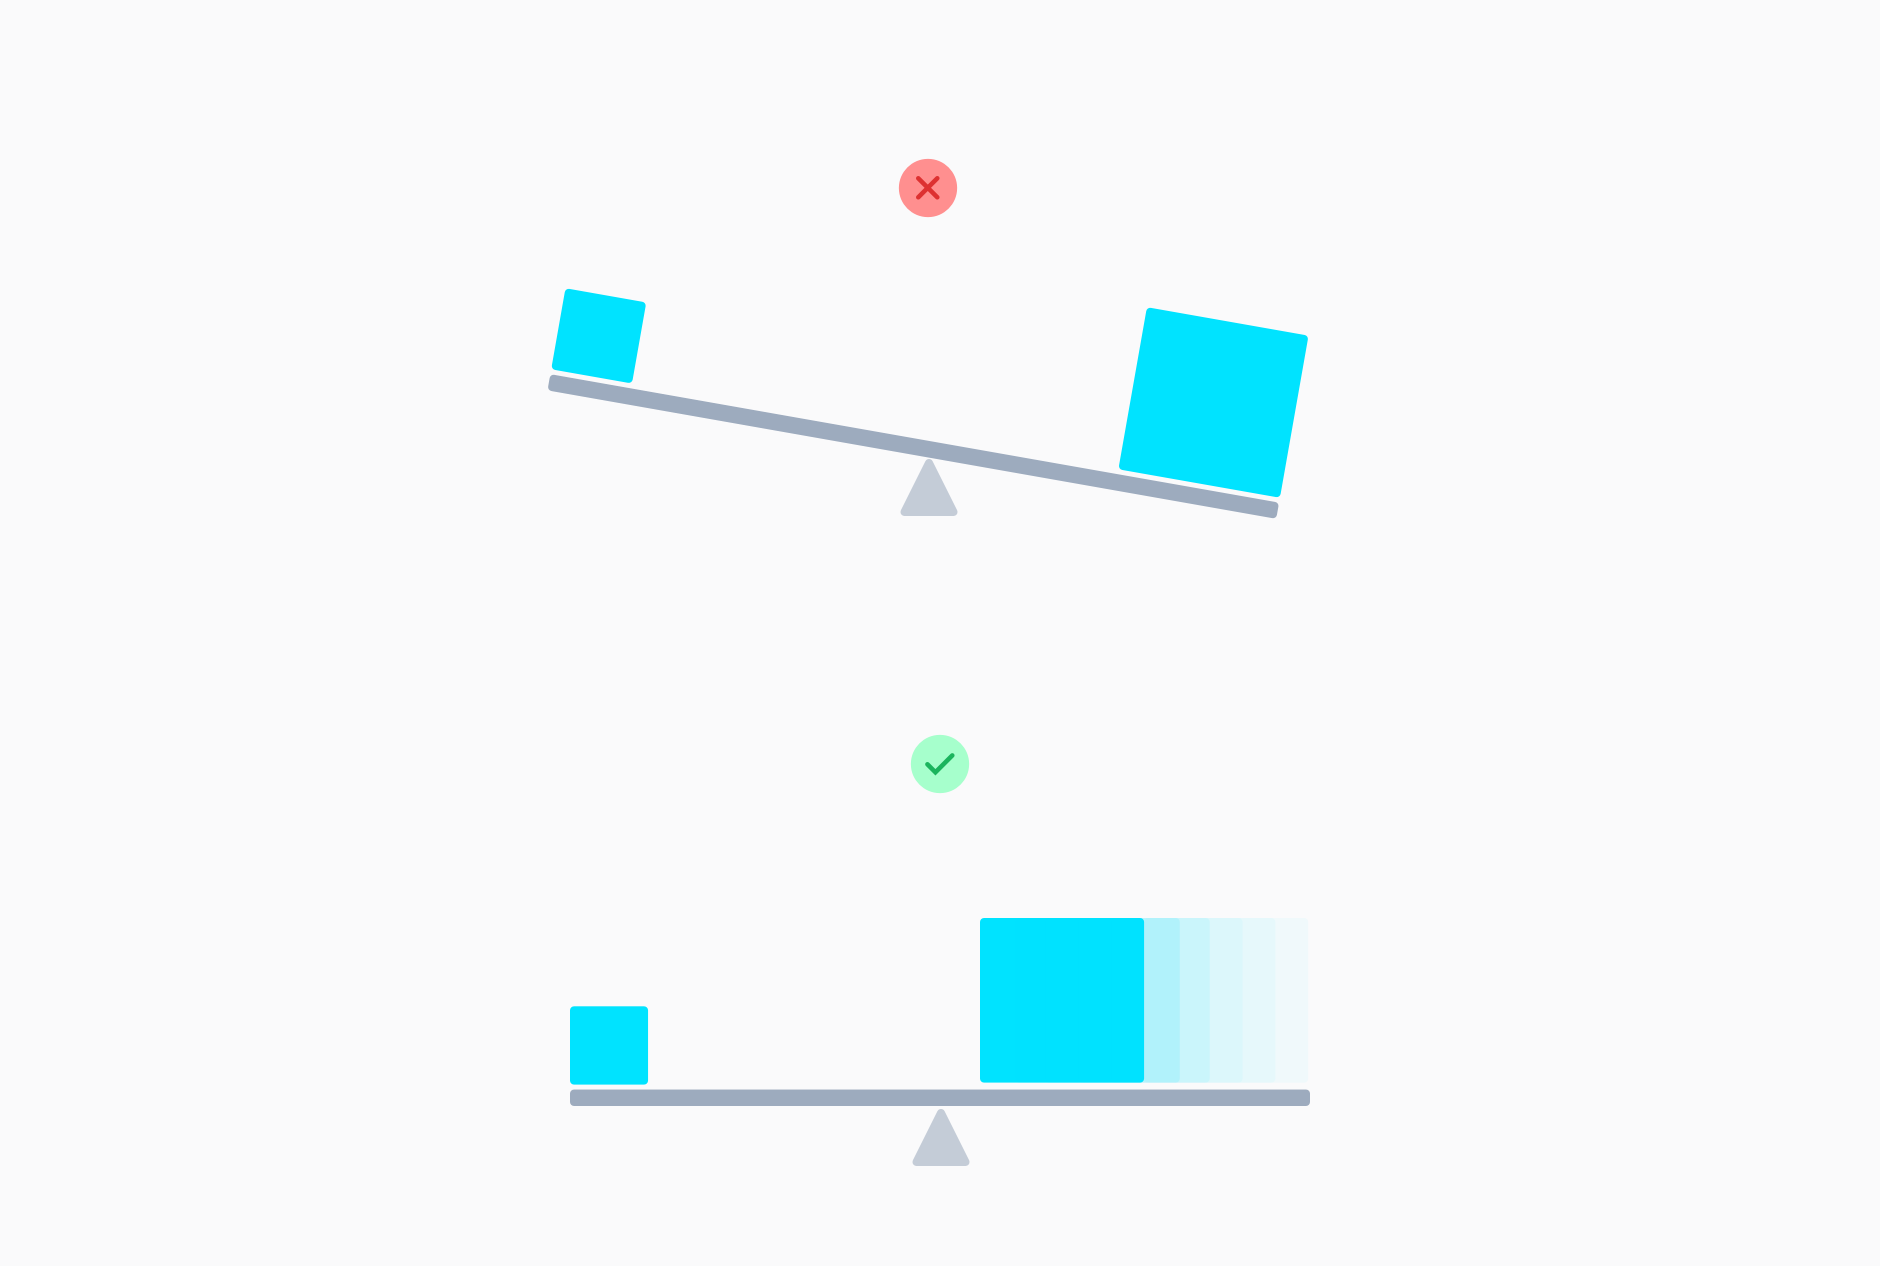
\includegraphics[width=10cm]{obrazky/rovnovaha_paka}\hfill
			\caption{Páka rovnováhy vzhledu. Zdroj: \cite{vizualni_rovnovaha}}
		\end{figure}

		Rozvržení prvků ale není vše, a je potřeba myslet i na samotný design.

		\paragraph{Paleta barev}

		Důležitou částí designu je správně připravená paleta barev, jenž bude použita napříč aplikací.
		Ta definuje jak obecné barvy prvků, jako jsou texty, bloky, tlačítka, tak i ty méně obecné.

		\begin{figure}[H]
			\centering
			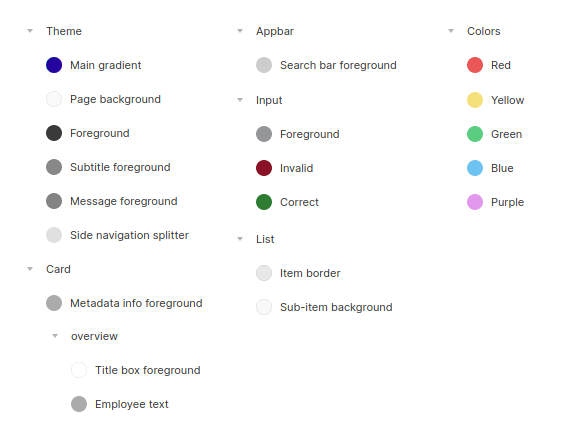
\includegraphics[width=\linewidth]{obrazky/paleta_barev}\hfill
			\caption{Navržená paleta barev. Zdroj: [autor]}
		\end{figure}

		\paragraph{Stíny a linky}

		Dalším velmi důležitým designovým prvkem jsou stíny pomáhající vizualizovat pomyslnou vzdálenost jednotlivých
		prvků od uživatelova zraku.
		Díky stínům je možné více se překrývajících prvků jasně ilustrovat uživateli, které prvky jsou více v
		popředí než ostatní.
		Způsobů používání stínu je mnoho.
		Pro tento projekt byl vybrán způsob, kdy se stín snaží simulovat reální stín generovaný světelným zdrojem.
		Na takové stíny jsou totiž uživatelé zvyklí z reálného světa.
		Velmi používané je i využití linek kolem jednotlivých prvků pro oddělení bloků.

		Tento projekt využívá kombinace linek a stínů.
		Stíny jsou v použity pro bloky ucelených informací a prvky, které mají vyšší prioritu než
		ostatní, a linky jsou použity pro prvky uvnitř bloků.
		Kombinace byla vybrána z důvodu zjednodušení vzhledu, protože použití pouze stínů by mohlo být pro některé uživatele
		příliš rozptylující.

		\begin{figure}[H]
			\centering
			
\includegraphics[width=8cm]{obrazky/ukazka_stinu_a_linek}
			\caption{Ukázka kombinace stínů a linek v jednom bloku. Zdroj: [autor]}
		\end{figure}

		\paragraph{Okraje}

		Kromě linek a stínu je dobré myslet i na samotné okraje prvků, tedy jesli budou mít zaoblené rohy či nikoliv.
		Po vzoru Material Designu byly zvoleny zaoblené rohy o průměru 8px pro větší lehkost prvků.
		Toto rozhodnutí je však celkem subjektivní a někteří uživatelé mohou preferovat ostré rohy.

		\begin{figure}[H]
			\centering
			
\includegraphics[width=8cm]{obrazky/blok_obsahu}\hfill
			\caption{Ukázka zaoblených rohů. Zdroj: [autor]}
		\end{figure}

		\paragraph{Signalizace výběru}

		Posledním pravidlem je zobrazování signalizace výběru.
		Tato část musí být pro koncové uživatele obzvlášť konzistentní a intuitivní napříč aplikací.
		Uživatel musí být schopen jednoznačně určit jaký prvek ze všech možných je vybraný.
		Velice používaným způsobem jak tuto signalizaci řešit je jednoduchá linka zobrazená u vybraného prvku.
		V rámci této aplikace byly navrženy dvě varianty: varianta pro pás prvků a varianta pro osamocené prvky.
		Varianta pro pás prvků se použije v případě pásu prvků, u kterých nemůže dojít k přetečení na více řádků.
		V takovém případě se použije jednoduchá linka pod či nad prvkem.
		V případě osamocených prvků nebo víceřádkových prvků je použita linka kolem celého okraje prvku.

		\begin{figure}[H]
			\centering
			
\includegraphics[width=6cm]{obrazky/ukazka_vyberu_1}\hfill
			\caption{Ukázka signalizace výběru v navigaci. Zdroj: [autor]}
		\end{figure}

		\begin{figure}[H]
			\centering
			
\includegraphics[width=4cm]{obrazky/ukazka_vyberu_2}\hfill
			\caption{Ukázka signalizace výběru konkrétního prvku. Zdroj: [autor]}
		\end{figure}

		\subsubsection{Strukturální prvky}

		Strukturálními prvky jsou myšlené takové prvky, které slouží jako základní stavební kameny pro jednotné
		rozvržení stránek.

			\paragraph{Blok obsahu}

			Stránky jsou rozvrženy hlavně pomocí tzv. bloků obsahu označující jeden logický celek informací
			na stránce.
			Blok obsahu vždy obaluje nějaký konkrétní obsah: dlouhý text, seznam položek, editor nebo cokoliv dalšího.
			Blok obsahuje hlavičku s nadpisem a lištou tlačítek, která dávají smysl pro celý logický celek.
			Samotný obsah těla už je pak záležitostí konkrétního využití bloku, avšak pravidlem je jednotné odsazení 24px od
			okrajů.
			Krajním případem je využití bloku bez hlavičky na speciálních stránkách s vlastním nadpisem, u nichž blok
			představuje logický celek informací platných pro celou stránku.

			\begin{figure}[H]
				\centering
				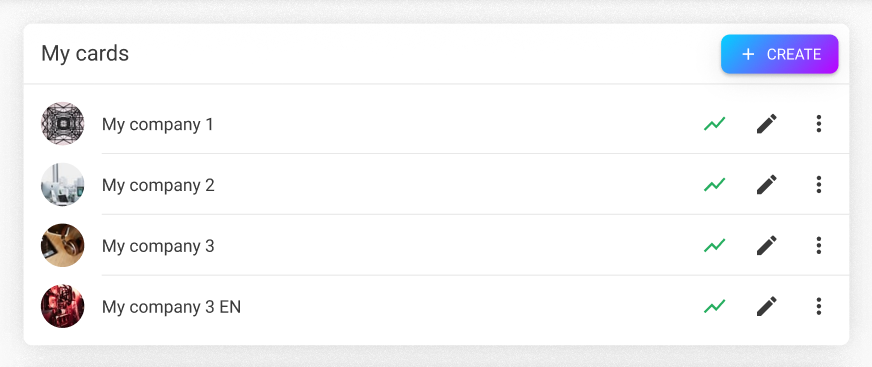
\includegraphics[width=\linewidth]{obrazky/blok_obsahu_ukazka}\hfill
				\caption{Ukázka využití bloku obsahu. Zdroj: [autor]}
			\end{figure}

			\paragraph{Lišta akcí}

			Kromě hlavní navigační lišty aplikace bylo nutné zavést ještě jeden typ lišty: lišta akcí.
			Díky ní je možné na určitých stránkách zobrazit sekundární lištu s nadpisem a dodatečnými akcemi, jenž se stahují
			k obsahu celé stránky.
			Takovými stránkami jsou většinou stránky zobrazující detail určitého objektu, se kterým lze manipulovat.

			\begin{figure}[H]
				\centering
				
\includegraphics[width=\linewidth]{obrazky/lista_akci}\hfill
				\caption{Ukázka lišty akcí. Zdroj: [autor]}
			\end{figure}

			\paragraph{Modální okno}

			Modální okna představují bloky obsahu, které při zobrazení překrývají všechen ostatní obsah, pro zdůraznění
			důležitosti.
			Jedná se především o potvrzení určitých akcí nebo zobrazení detailu nějakého objektu.
			Každé okno má hlavičku, a případně i patičku, avšak obsah se mění podle typu okna.
			Tato aplikace rozlišuje dva primární typy oken: informační a akční okno.
			Informační okno slouží k zobrazení již existujících dat a nevyžaduje od uživatele žádnou akci.
			Lze ho zavřít buď křížkem v hlavičce nebo kliknutím mimo okno, a neobsahuje patičku.
			Akční okno akci vyžaduje a uživatel musí vždy nějakou akci zvolit, nelze okno zavřít pouhým kliknutím mimo okno.
			Takové okno má v hlavičce pouze nadpis a obsahuje patičku se všemi dostupnými akcemi.
			Příkladem takových akcí může být potvrzení vytvoření objektu nebo zrušení operace.
			Tlačítko nejdůležitější akce je patřičně odlišeno od běžných tlačítek, aby bylo zřejmé, co se po
			uživateli chce.

			Okna mají podobná pravidla odsazení jednotlivých vnitřních prvků jako bloky obsahu.
			Obsah by měl být odsazen 24px od okrajů okna (až na výjimky s vlastním odsazením) a akční tlačítka jsou
			mezi sebou odsazeny 8px.
			Celá patička je navíc pro jasné rozdělení částí rovněž odsazena 24px.

			\begin{figure}[H]
				\centering
				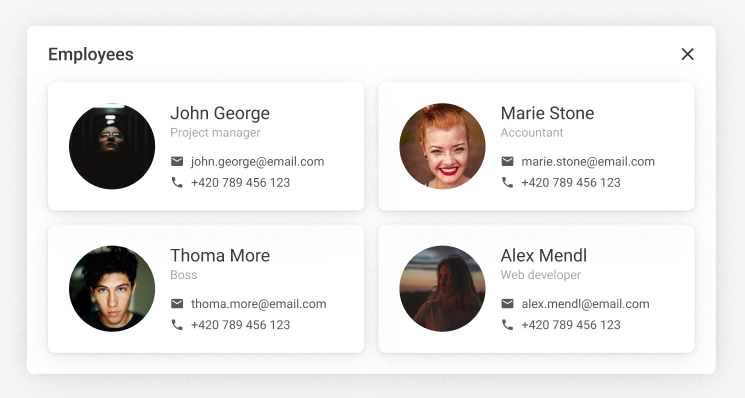
\includegraphics[width=10cm]{obrazky/modalni_okno_informacni_ukazka}\hfill
				\caption{Ukázka konkrétního informačního modální okna. Zdroj: [autor]}
			\end{figure}

			\begin{figure}[H]
				\centering
				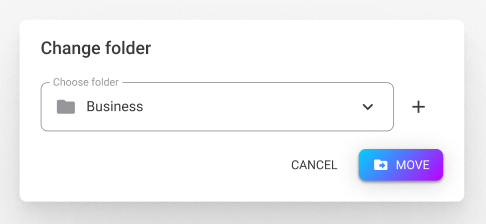
\includegraphics[width=10cm]{obrazky/modalni_okno_akcni_ukazka}\hfill
				\caption{Ukázka konkrétního akčního modálního okna. Zdroj: [autor]}
			\end{figure}

			\paragraph{Kontextuální nabídka}

			Jedná se malé menu zobrazující rozšířené možnosti nějaké akce.
			Většinou se používá, pokud není v \ac{UI} dostatek
			místa pro všechny dostupné akce, nebo pro výběr konkrétní položky z výběrového pole ve formuláři.

			\begin{figure}[H]
				\centering
				
\includegraphics[width=8cm]{obrazky/kontextualni_nabidka_seznam_ukazka}\hfill
				\caption{Ukázka kontextuální nabídky akcí položky v seznamu. Zdroj: [autor]}
			\end{figure}

		\subsubsection{Prvky pro interakci}

		Po prvcích strukturující obsah je možné navrhnout prvky, se kterými bude uživatel přímo či nepřímo interagovat.

			\paragraph{Tlačítko}

			Nejhlavnějším takovým prvkem je tlačítko.
			To umožňuje uživatelům vyvolávat akce, potvrzovat akce nebo se nechat přesměrovat na jiné stránky.
			Tlačítek je v aplikaci spousta a každé dělá trochu něco jiného.
			Lze je ale zařadit do pár kategorií, a navrhnout tak několik obecných typů tlačítek.
			Všechny tlačítka byla rozdělena na tlačítka s nízkou prioritou, vysokou prioritou a vysokou vážností akce.

			Tlačítko s nízkou prioritou reprezentuje vedlejší akci, kterou sice uživatel může provést, ale jeho není hlavním cílem.
			Takové tlačítko má neutrální barvu a ve většině případech neobsahuje ani ikonu

			\begin{figure}[H]
				\centering
				
\includegraphics[width=4cm]{obrazky/tlacitko_s_malou_prioritou}\hfill
				\caption{Ukázka tlačítka s malou prioritou. Zdroj: [autor]}
			\end{figure}

			Tlačítko s vysokou prioritou představuje primární akci, kterou by se uživatel měl vydat.
			Taková tlačítka představují potvrzení nějaké akce, vytvoření nových objektů, přidání existujících objektů a
			podobně.
			Měla by být proto patřičně zvýrazněna a uživatele podvědomě navádět.
			Z tohoto důvodu mají tlačítka výraznou barvu a vystihující ikonu.

			\begin{figure}[H]
				\centering
				
\includegraphics[width=4cm]{obrazky/tlacitko_s_velkou_prioritou}\hfill
				\caption{Ukázka tlačítka s vysokou prioritou. Zdroj: [autor]}
			\end{figure}

			Pro případy, kdy uživatel provádí nějakou akci s vysokou vážností, jako je například nevratné smazání nějakého
			objektu, vzniklo rozšíření tlačítka s vysokou prioritou.
			Tlačítko se liší pouze v červené barvě evokující dojem závažné akce.

			\begin{figure}[H]
				\centering
				
\includegraphics[width=4cm]{obrazky/tlacitko_s_velkou_prioritou_a_velkou_vaznosti}\hfill
				\caption{Ukázka tlačítka provádějící nevratnou změnu. Zdroj: [autor]}
			\end{figure}

			\paragraph{Vstupní pole}

			Vstupní pole různých druhů jsou společně s tlačítky nejdůležitějšími prvky jakékoliv aplikace.
			Vstupní pole umožňují uživatelům předat data aplikaci v různých formátech.
			Vzniklo proto několik základních typů vstupních polí, které lze jednoduše kombinovat uvnitř v formulářů.
			Mezi ně patří: textová pole, výběrová pole, pole pro výběr času a data, pole pro nahrání obrázku a pole pro
			výběr geografické lokace.
			Vstupní pole využívají linek namísto stínů, protože reprezentují pouze část celého bloku.
			Pole mají popisek pro identifikaci účelu konkrétního pole, ikonu a mohou mít i akční tlačítko.
			Pod pole je navíc možné vepsat nápovědu.

			Textová pole slouží pro zadávání krátkých i dlouhých textů, mají vždy popisek a mohou mít ikonu a
			akční tlačítko.

			\begin{figure}[H]
				\centering
				
\includegraphics[width=8cm]{obrazky/textove_pole}\hfill
				\caption{Ukázka textového pole s ikonou a nápovědou. Zdroj: [autor]}
			\end{figure}

			Extenzí textového pole jsou pole pro zadání času a data.
			Ty rozšiřují manuální zadávání o okénka pro pohodlný výběr bez nutnosti klávesnice.

			\begin{figure}[H]
				\centering
				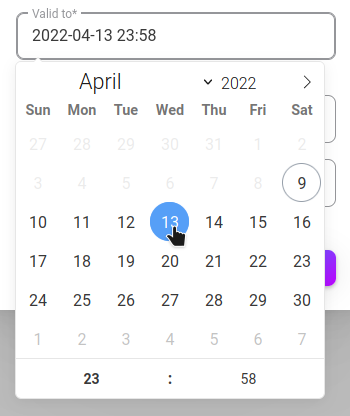
\includegraphics[width=6cm]{obrazky/datumove_pole}\hfill
				\caption{Ukázka pole s výběrem data a času. Zdroj: [autor]}
			\end{figure}

			Vzhledem k požadavku specifikovat geografické lokace karet, bylo potřeba zavést i specifická pole
			pro výběr bodů v mapě.
			Pole zobrazuje mapu světa, se kterou je možné hýbat, přibližovat ji a vybírat konkrétní body.

			\begin{figure}[H]
				\centering
				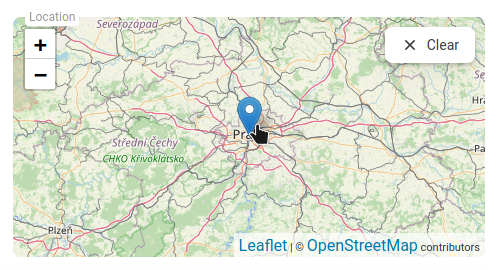
\includegraphics[width=8cm]{obrazky/pole_lokace}\hfill
				\caption{Ukázka pole pro výběr geografického bodu v mapě. Zdroj: [autor]}
			\end{figure}

			Posledním méně používaným polem v této aplikaci je pole pro výběr obrázku.
			Pole umožní výběr souboru ze souborového systému uživatele, který je následně nahrát a zobrazen jeho náhled
			přímo v poli.
			Vybraný obrázek je pak možné jednoduše změnit nebo úplně odstranit.

			\begin{figure}[H]
				\centering
				
\includegraphics[width=5cm]{obrazky/obrazkove_pole}\hfill
				\caption{Ukázka pole s nahraným obrázkem. Zdroj: [autor]}
			\end{figure}

			\paragraph{Seznam položek}

			Velmi využívaným prvkem je seznam položek.
			Každá položka může obsahovat ikonu nebo obrázek, text, seznam akcí, nebo dokonce i vnořený další seznam.
			Akce položek se kromě běžného zobrazení umí v případě malého místa seskupit a schovat do kontextuální
			nabídky, aby uživatel využívající malé zařízení nepřišel o možnost využívat všechny akce.

			\begin{figure}[H]
				\centering
				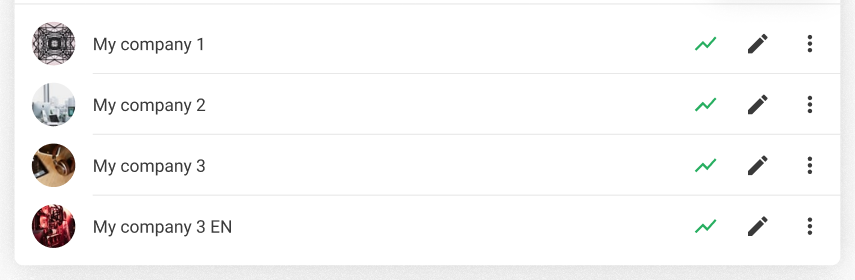
\includegraphics[width=\linewidth]{obrazky/seznam}\hfill
				\caption{Ukázka pokročilého seznamu prvků. Zdroj: [autor]}
			\end{figure}

			\paragraph{Stránkování}

			Při velkém množství položek v jednom seznamu se využívá systém stránkování.
			Prvek stránkování umožňuje přepínat mezi konkrétními stránkami, nebo se přepínat mezi předchozí a následující stránkou.

			\begin{figure}[H]
				\centering
				
\includegraphics[width=4cm]{obrazky/strankovani}\hfill
				\caption{Ukázka stránkování. Zdroj: [autor]}
			\end{figure}

		\subsubsection{Finální návrh}

		S pomocí výše navržených prvků a jejich variacemi, bylo navrženo finální \ac{UI} všech stěžejních
		stránek.

		\begin{figure}[H]
			\centering
			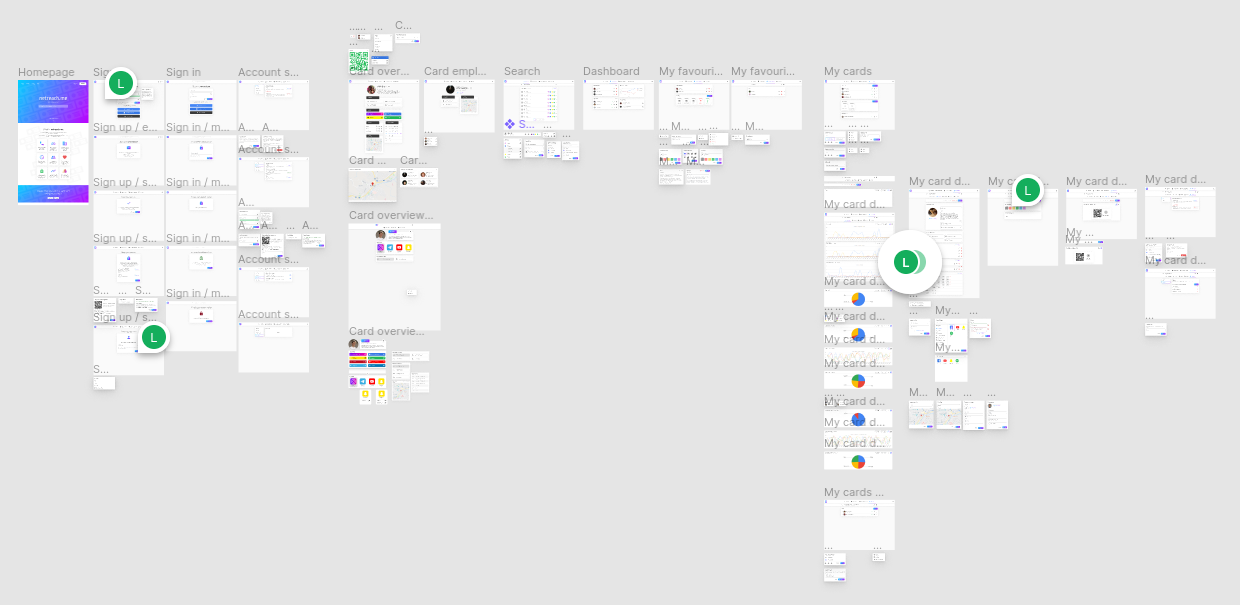
\includegraphics[width=\linewidth]{obrazky/finalni_navrh}\hfill
			\caption{Finální grafický návrh aplikačních stránek a prvků. Zdroj: [autor]}
		\end{figure}

		Tento postup se ukázal jako velmi efektivní oproti původnímu prototypu, protože
		pomohl snadněji implementovat samotné \ac{GUI} a navrhnout \ac{API} díky zřetelným funkčním požadavkům.

	\subsection{Implementace API serveru}

		\subsubsection{Datový model}

		Úkol \ac{API} serveru je poskytovat a zpracovávat data, ať už textová v podobě \ac{JSON} dokumentů, nebo binární v podobě
		obrázků.
		Tyto funkce pro samotné API bude zprostředkovávat implementovaná business logika starající se o to, aby všechna data
		byla správně zpracována a uložena.
		Je ale stěžejní se na počátku zamyslet, vybrat styl a navrhnout model, jakým bude business logika implementována.
		Stěžejní je to z důvodu budoucí čitelnosti kódu a možnostech rozšíření o nové funkce.

		Vzhledem k tomu, že byl vybrán jazyk Java, který je primárně objektově orientovaným programovací jazykem, business
		logika bude využívat právě principů \ac{OOP}.
		\ac{OOP} je velice populární a většinově používané programovací paradigma využívané spoustou programovacích
		jazyků.
		Toto paradigma využívá objekty pro sestavení systému.
		Každý objekt má nějaké své vlastnosti a operace, které může buď využívat vnitřně nebo poskytnout ostatním
		objektům.
		Hlavní myšlenka \ac{OOP} je popisovat reálné objekty (člověk, pes, budova, událost...) těmi virtuálními ve zjednodušené
		formě, v níž popisujeme jen tu část reálného objektu, která nás zajímá.
		Tyto objekty pak v systému mezi sebou komunikují pomocí zpráv a předávají si data tak, aby dosáhly výsledku.
		Každý objekt v systému má svou předlohu zvanou třída jenž definuje podporované vlastnosti a operace.
		Kromě tříd ještě existují rozhraní a abstraktní třídy, které můžou mezi sebou dědit vlastnosti a operace.
		Rozhraní a abstraktní třídy definují obecnou předlohu operací, tzv. kontrakt, které dědící třída musí splňovat, což
		následně umožňuje využít techniku polymorfismus, tedy provádět operace na základě obecného rozhraní bez nutnosti
		znát konkrétní třídu.
		\cite{oop}

		Právě díky \ac{OOP} bylo možné poměrně věrně reprezentovat objekty využívané jednotlivými stránkami v logické,
		přehledné a jasně definované struktuře.
		Model byl pro přehlednost interně rozdělen na několik modulů podle zaměření, nicméně všechny moduly
		mezi sebou i tak komunikují.
		Momentálně se datový model skládá z modulu pro správu uživatelských účtů, modulu pro správu karet, modulu pro správu a
		kupónů.

		\paragraph{Model uživatelských účtů}

		Modul uživatelských účtů je zodpovědný za vytváření, uchování, úpravu a mazání jednotlivých účtů.
		S tím je spojena i správa oblíbených karet a poznámek, které jsou vázány na konkrétního uživatele.
		Modul dál řeší i prémiový plán a předplatné.

		\begin{figure}[H]
			\centering
			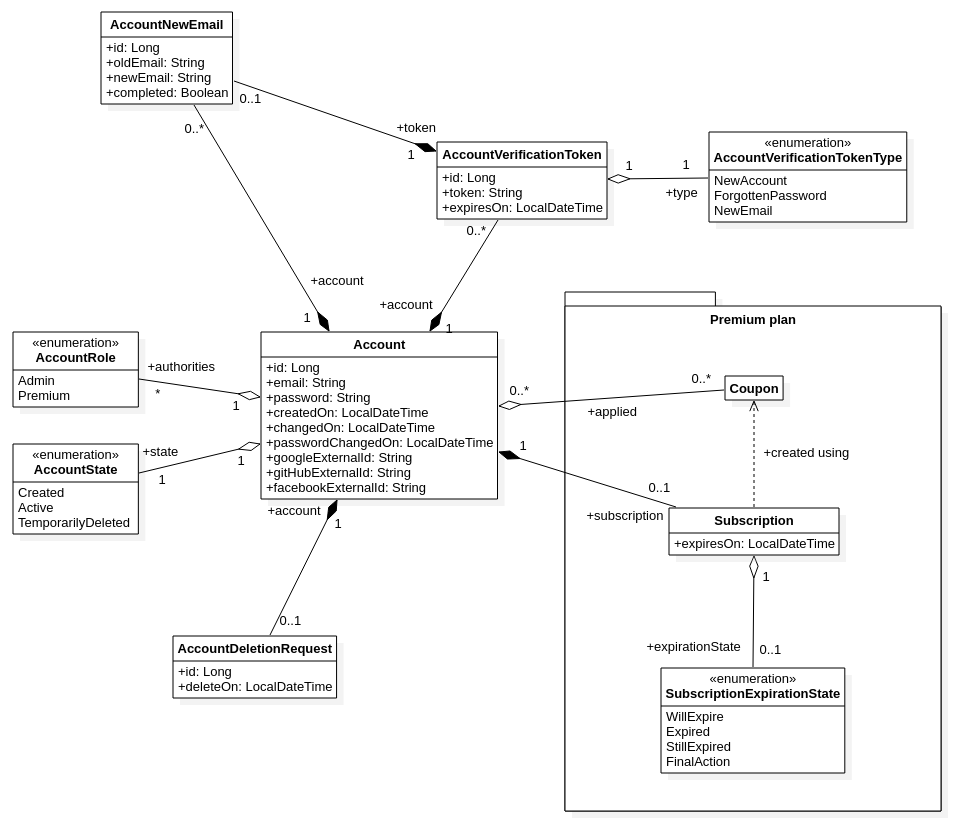
\includegraphics[width=\linewidth]{obrazky/datovy_model_ucet}\hfill
			\caption{Datový model popisující uživatelské účty. Zdroj: [autor]}
		\end{figure}

		Jak je možno vidět z diagramu, účet má kromě základních přihlašovacích informací i spoustu
		doplňujících dat.

		V první řadě, každý účet má přiřazený vždy nějaký stav.
		Při vytvoření má nový účet stav \emph{Created} vyjadřující nový a zatím neaktivovaný účet.
		Tento účet nelze využívat.
		Po aktivaci se změní stav účtu na \emph{Active}, který říká, že účet je již aktivovaný, a tedy plně použitelný.
		Poslední stav \emph{TemporarilyDeleted} označuje dočasné smazaný účet, což znamená, že je naplánováno jeho permanentní
		smazání.
		To umožňuje uživatelům v omezené lhůtě svůj účet obnovit.

		Další velmi důležitou komponentou je systém ověřovacích tokenů sloužících k potvrzování akcí, kde
		je potřeba ověřit, že akci provádí skutečný uživatel nikoliv podvodník.
		Tokeny jsou pseudo náhodně generované unikátní textové řetězce přiřazené vždy k jednomu určitému uživateli.
		Typ tokenu pak říká, co daný token ověřuje.
		Ověřitelnou akcí může být aktivace nového účtu, změna emailové adresy nebo zapomenuté heslo.
		V případě tokenu pro změnu emailové adresy se nová emailová adresy se ukládá mimo samotný účet k danému tokenu.
		Díky tomu je možné emailovou adresu změnit, až ve chvíli, kdy byl token ověřen, a zároveň je možné v případě
		odcizení účtu zobrazit historii všech změn.

		Systém dále pracuje s rolemi udávajícími obecná práva uživatele.
		Každé obecné roli jsou přiřazena nějaká práva v systému (čtení, modifikace...), a pokud uživatel má takovou roli
		přiřazenou, automatický dědí její práva.
		Toto je poměrně jednoduchý a efektivní systém práv.
		Momentálně systém pracuje s administrátorskou rolí a prémiovou rolí.
		Administrátorská role uděluje uživateli práva pro přístup do interní administrační části
		aplikace, pomocí které je možné spravovat provoz aplikace.
		Druhou rolí je role prémiová, která je určena pro běžné uživatele, a odemyká jim prémiové funkce aplikace.
		Tato role vzniká automaticky při vytvoření předplatného a zaniká s jeho expirací.

		Pro plánované mazání účtů se uchovává požadavek s informací o tom, jaký účet bude smazán, a kdy dojde k permanentnímu
		smazání společně s jeho daty.

		Poslední hlavní částí uživatelských účtů jsou komponenty pro prémiové funkce.
		Jedná se především o popisný objekt předplatného.
		Ten vzniká aktivací prémiovýho plánu a říká, že účet má práva na prémiové funkce.
		V jistých případech může mít přiřazený i datum expirace, se kterým automaticky zanikne.
		S tím se váže i stav expirace, která pomáhá upozorňovat uživatele na současný stav předplatného.

		\paragraph{Model kupónů}

		\begin{figure}[H]
			\centering
			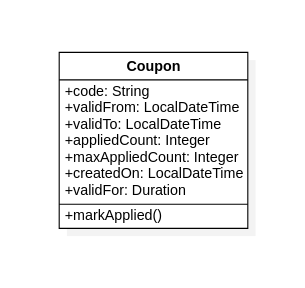
\includegraphics[width=6cm]{obrazky/datovy_model_kupon}\hfill
			\caption{Datový model kupónového systému. Zdroj: [autor]}
		\end{figure}

		Předplatné může vzniknout na základě zadání platného kupónu, avšak systém kupónů je navržen obecně, aby
		bylo možné ho v případě budoucích rozšíření jednoduše přepoužít i na aktivaci jiných funkcionalit, ne jen
		pro prémiové plány.
		Každý kupón musí mít unikátní kód, buď vygenerovaný nebo zadaný správcem.
		Mimo to má definovanou platnost, maximální počet možných aplikování a dobu po jakou bude vytvořené předplatné platné.

		\paragraph{Model karet}

		\begin{figure}[H]
			\centering
			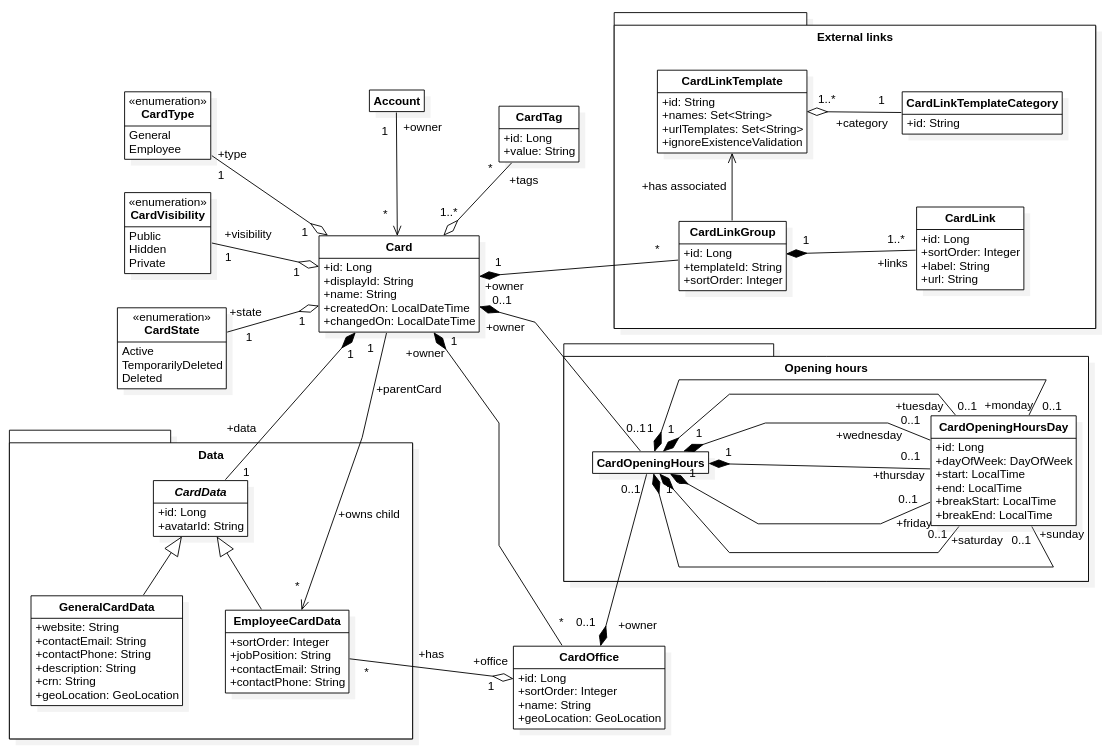
\includegraphics[width=\linewidth]{obrazky/datovy_model_karta}\hfill
			\caption{Datový model karet a navázaných dat. Zdroj: [autor]}
		\end{figure}

		Nejhlavnějším prvkem v této aplikaci jsou samotné karty a jejich data.
		Každá karta má v prvé řadě vždy nějakého vlastníka, který má jako jediný práva na
		úpravu.

		Samotná karta je rozpadnuta do několika částí pro podporu více typů karet.
		Srdcem je jednoduchá třída popisující pouze obecná metadata, která jsou potřeba pro všechny typy karet.
		V této třídě je tedy zahrnut vlastník, typ, viditelnost, stav, veřejné jméno, tzv. "display ID" a další metadata.
		Display ID je unikátní textové ID karty určené primárně pro koncové uživatele.
		Toto ID je totiž zobrazováno v \ac{URL} adrese konkrétní karty a má za cíl umožnit jednoduše sdílet karty bez nutnosti
		znát kryptické náhodně generované číselné identifikátory.
		Toto ID může být definováno ručně uživatelem nebo generováno aplikací (vhodné pro skryté karty).
		Typ karty definuje jak s danou kartou lze pracovat a jaká data poskytuje.
		Momentálními typy jsou obecná karta a karta zaměstnance, avšak tento systém dovoluje poměrně jednoduché rozšiřování
		o nové typy karet.
		Obecné karty je možné tvořit uživateli přímo a podporují všechny typy údajů.
		Původně byl tento typ rozdělen ještě na osobní a firemní kartu, nicméně jediný rozdíl bylo omezení podporovaných dat
		v osobních kartách.
		Tento přístup však přinášel mnoho duplicit, a zároveň znemožňoval uživatelům osobních karet využívat funkce
		firemních karet, jenž za určitých okolností dávaly smysl i u osobních karet (např.: pro OSVČ).
		Právě kvůli těmto nevýhodám a žádným jasným výhodám, byly tyto dva typy sjednoceny, především pro pohodlí
		koncových uživatelů.
		Karty zaměstnanců se pak tvoří nepřímo jako hierarchičtí potomci obecných karet v editaci nadřazené karty, a
		obsahují specifická data pouze pro zaměstnance.
		Posledním důležitým metadatem je viditelnost specifikující, kdo může danou kartu vidět.
		Veřejné karty může navštívit a vyhledat kdokoliv.
		Skryté může navštívit pouze uživatel disponující konkrétní \ac{URL} adresou odkazující na danou kartu.
		Privátní karta pak už slouží pouze pro autora karty.

		Každé kartě lze přiřadit libovolné množství štítků pro kategorizaci.
		Štítky jsou uživatelsky definované, a můžou tak obsahovat cokoliv.
		Navíc jsou znovupoužitelné, takže více karet může být označeno stejným štítkem.

		Pro definování informací o kartě existuje koncept napojených dat.
		Tyto data reprezentují soubor údajů, které daný typ karty podporuje.
		Každý typ karty má svoji implementaci těchto dat.
		Je pak na business logice aplikace, aby dokázala s daty správně pracovat.
		Tato obecnost umožňuje jednoduše vytvářet nové typy karet s úplně odlišnými daty, aniž by se data musela míchat
		a být nepřehledná.

		Pro většinu karet pak pravděpodobně budou nejdůležitějšími daty \ac{URL} odkazy na externí webové stránky,
		především na sociální sítě.
		Ty z karet dělají jakési rozcestníky pro objevení profilů subjektů na sociálních sítích.
		Každý jeden odkaz má originální cílovou \ac{URL} adresu, popisek a pořadí mezi ostatními odkazy na stejné úrovni.
		Popisek slouží především pro odlišení více odkazů vedoucí na stejnou webovou stránku.
		\ac{URL} adresa je hlavní informace a z důvodu bezpečnosti musí být validována oproti zvolené šabloně sítě.
		Díky tomu není možné vytvořit odkaz pod jednou sítí, ale odkazovat na podvodnou.
		Jednotlivé odkazy jsou pak seskupovány do skupin odkazů vycházející ze stejné šablony.
		I přes to, že skupiny zastřešují vždy nějaký soubor sítí stejného typu, může existovat více skupin vycházející ze
		stejné šablony.
		To umožňuje poměrně velkou flexibilitu struktury odkazů a neomezuje uživatele na jeden odkaz pro jednu síť (což je
		nevýhoda některých konkurenčních řešení).
		Jednotlivé šablony jsou reprezentovány separátními konfiguračními třídami.
		Z návrhu vyplývá potřeba definovat názvy, podle kterých lze šablony vyhledat, a platné šablony \ac{URL} odkazů
		oproti kterým se validují konkrétní cílové \ac{URL} adresy.
		Stejně jako názvů, může být i více šablon \ac{URL} adres, protože většina webových stránek podporuje více domén třetího řádu,
		a je tak nutné definovat všechny, protože není jasné jakou \ac{URL} adresu uživatel zadá.
		Každá taková šablona je pak zařazena do jedné nebo více kategorií sloužící čistě pro jednodušší vyhledávání.

		Pro firmy poměrně užitečnou informací může být jejich hierarchie poboček a zaměstnancům, zejména u větších společností.
		Proto každá obecná karta může mít libovolné množství přiřazených poboček/kanceláří/prodejen, kde každá má své jméno
		a geografickou lokaci.
		Ke každé takové pobočce je možné přiřadit zaměstnanecké karty.
		Kromě zaměstnanců může mít pobočka i vlastní otevírací dobu.

		Velmi důležitou informací pro potencionální zákazníky je aktuální otevírací doba.
		Byl proto navržen obecný model otevírací doby, který lze navázat na jakoukoliv jinou entitu.
		Model je zastřešen jednou třídou seskupující otevírací dobu jednotlivých dnů v týdnu.
		Každý den má pak definovaný interval, kdy má daná entita otevřeno, kdy má přestávku.

		\paragraph{Model oblíbených karet}

		\begin{figure}[H]
			\centering
			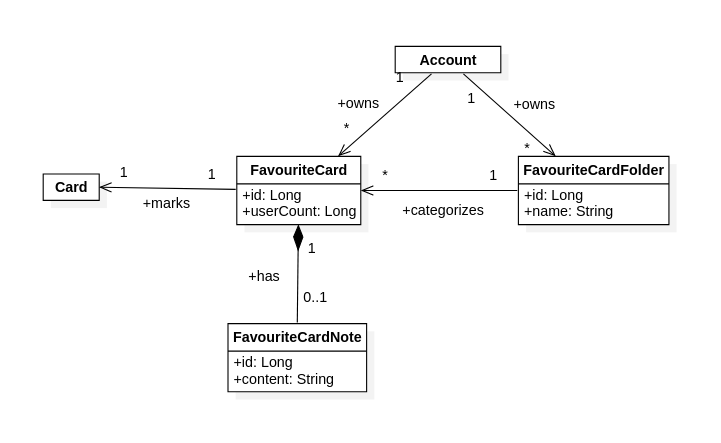
\includegraphics[width=\linewidth]{obrazky/datovy_model_oblibene_karty}\hfill
			\caption{Datový model oblíbených karet uživatelských účtů. Zdroj: [autor]}
		\end{figure}

		Oblíbené karty umožňují k uživatelskému účtu přiřazovat cizí karty jako oblíbené.
		Každý účet může jako oblíbené označit libovolný počet karet, což danému uživateli umožní rychlý přístup
		k požadovaných informacím.
		Každá oblíbená karta navíc může mít jednu textovou poznámku s formátováním.
		Oblíbené karty je pak možné seskupovat do složek definovaných uživatelem pro lepší orientaci.
		Složky, poznámky ani oblíbené karty však nevidí nikdo jiný než autor.

		\subsubsection{Práce s datovým modelem}

		Práci s datovým modelem zastřešuje právě již několikrát zmíněná business logika.
		Struktura business logiky si bere inspiraci z návrhového vzoru \ac{DDD}, který se zabývá
		navrhováním přehledné, znovu použitelné a hlavně jednoduše rozšiřitelné struktury, řešící zadané businessové požadavky
		projektu.
		Tento vzor pohlíží na problematiku jako na doménu, a staví hlavně na konceptu služeb,
		což jsou speciální třídy, které
		neudržují vnitřní stav, ale poskytují služby manipulující s datovými objekty \cite{ddd_quickly}.
		Jednotlivé služby by se měli vždy zabývat pouze jedním typem dat kvůli přehlednosti, a ostatní data delegovat na
		ostatní služby \cite{ddd_quickly}.
		Druhým podstatným stavebním blokem jsou repozitáře zajišťující předávání dat mezi aplikací a databázovým systémem
		\cite{ddd_quickly}.
		\ac{DDD} obsahuje spoustu dalších konceptů, nicméně ty byly při implementaci využity jen vzdáleně.
		Implementovaná business logika má tak několik službových tříd a repozitářů.
		Pro každou separátní část modelu existuje manipulující služební třída a jeden repozitář starající se především o
		načítání a ukládání dat do databáze.
		Konzumující logika si pak může vybrat přesně s jakými daty chce pracovat.
		Zatímco repozitáře se starají pouze o komunikaci s databází pomocí \ac{SQL} jazyka,
		služební třídy tyto informace předávají dál, upravují nebo validují.

		\begin{figure}[H]
			\centering
			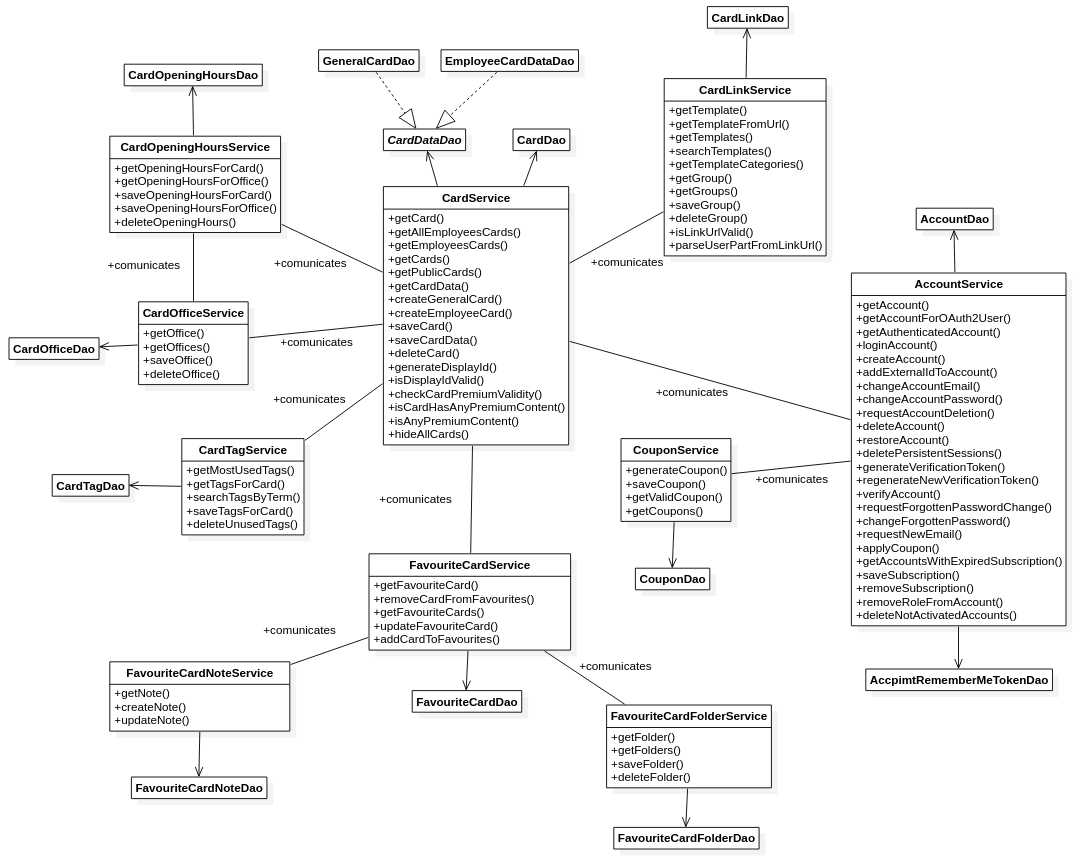
\includegraphics[width=\linewidth]{obrazky/sluzby_a_repozitare}\hfill
			\caption{Zjednodušený model služeb a repozitářů. Zdroj: [autor]}
		\end{figure}

		Momentální implementace služeb komunikuje mezi sebou převážně pomocí primárních klíčů jednotlivých entit, aby
		bylo zaručeno, že entita, se kterou služba manipuluje je vždy aktuální verzí reflektující stav databáze.
		Nicméně tento přístup značně zesložiťuje závislost tříd na jiné třídy, což vede k složitějšímu
		instanciování a testování tříd.

		Bohužel, při postupném rozšiřování aplikačních požadavků se ukázalo, že rozpad logických celků entit není úplně
		vhodný, a i když funguje bez problémů, jeho testování a nastavování je složité.
		Tento problém však řeší právě návrhový vzor \ac{DDD} svými entitami a hodnotovými objekty.
		Podle tohoto vzoru by se mělo pracovat s logickými celky jako s jednou entitou, aby se předešlo výše zmíněné složitosti
		rozpadlosti služebních tříd.
		Další podstatnou výhodou této provázanosti je zaručení konzistentnosti dílčích entit.
		Implementovaný přístup tento problém také řeší, a to pomocí validací, nicméně kvůli
		nutnosti se stále dotazovat na stav nadřazených entit složitost rapidně stoupá.
		\cite{ddd_quickly}
		Pro momentální stav aplikace je implementovaný model dostačující, nicméně pro budoucí rozšíření by bylo nutné
		model značně optimalizovat pomocí \ac{DDD} vzorů.

		\subsubsection{Komunikace s databázových systémem}

		Prvním problémem k řešení při implementaci již samotné business logiky mapování objektů do databázové struktury.

		V případě, že by aplikace využívala nějakou z \ac{NoSQL} databází s podporou \ac{JSON} dokumentů, by bylo toto
		mapování poměrně jednoduché.
		Jedinou složitost by pravděpodobně představovalo mapování hierarchických karet.

		V případě vybrané \ac{SQL} databáze je ale problém složitější, protože tyto databáze pracují s tabulkami místo objekty.
		Na první pohled se může zdát, že by to neměl být velký problém, protože sloupce tabulek jsou podobné atributům
		objektů.
		Složitost je hlavně v načítání a ukládání komplexních entity složených z více objektů a kolekcí, hlavně pak
		kolekcí 1:N (případně M:N).
		Jazyk \ac{SQL} totiž neumožňuje jednoduše vrátit více řádků z jiných tabulek, a tak není možné najednou
		vrátit objekty různých tříd tvořící jeden celek.
		Stejný problém je i v případě ukládání dat, při němž \ac{SQL} umožňuje ukládat pouze řádky do jedné tabulky.
		Ještě horší je to v případě ukládání již existujících dat, protože \ac{SQL} neumožňuje hromadné úpravy.

		Naštěstí existuje několik knihoven a nástrojů, které tyto problémy řeší za programátora.
		Je však možné vše implementovat ručně, to je ale zdlouhavé a zbytečné.
		Mezi nejpoužívanější knihovny patří Hibernate a MyBatis.
		Poměrně novou zajímavou alternativou je Spring Data JDBC, bohužel tato knihovna v době vývoje nebyla příliš
		rozšířená a neosvědčená na to, aby se dostala do výběru.

		Hibernate a MyBatis mají dost rozdílné přístupy k řešení výše zmíněných problémů.
		Zatím co Hibernate se snaží být plným \ac{ORM} frameworkem a odstínit programátora od jakéhokoli
		\ac{SQL} jazyka \cite{hibernate_docs}, MyBatis je lehčí alternativa, která poskytuje pouze nástroje pro mapování a dotazování, ale
		nezatěžuje programátora všemi nízkoúrovňovými problémy \cite{mybatis_getting_started}.
		Další velký rozdíl jakým knihovny pracují s entitami na pozadí.
		Hibernate využívá mezičlánku mezi repozitářem a databází, kde jsou dočasně entity uloženy \cite{hibernate_docs}.
		Díky tomu je Hibernate schopen poskytovat mezipamět pro entity při vícenásobném dotahování, a při ukládání
		se data nepromítají hned, ale až na konci transakce \cite{hibernate_docs}.
		Kvůli tomu se tak repozitář chová spíše jako paměťové úložiště, v němž má programátor okamžitý přístup k objektům.
		Bohužel to má i svá úskalí, a to nejen v celkové komplexitě knihovny.
		Úskalí se skrývá, hlavně pro tento projekt, ve sdílení instancí jedné entitu při vícenásobném
		dotažení entity z databáze.
		Tento přístup zamezuje porovnávání originální verze entity a nové upravené (většinou přijaté skrze \ac{API}),
		protože interně ji Hibernate považuje za jednu instanci.
		Hibernate sice má dobré nástroje pro validaci entit, ty však validují pouze aktuální hodnoty v objektech, ale
		není možné porovnat hodnoty s původními verzemi entit.
		To je v případě, kdy má entita vlastnosti, které se nesmí změnit, poměrně limitující.
		Instance entity sice lze vyjmout z Hibernatu, to je však poměrně složité.
		MyBatis tento neduh nemá a vrací vždy novou instanci entity.
		MyBatis se nesnaží řešit vše, a díky tomu je jeho abstrakce mnohem jednodušší.
		To ovšem znamená, že programátor musí odvést více práce při mapování a psát \ac{SQL} dotazy.
		Musí také ručně řešit ukládání složených entit, což Hibernate řeší sám.

		I když by se mohlo zdát, že Hibernate je ultimátním nástrojem pro 99\% projektů, existuje mnoho materiálů
		zkušených programátorů využívajících Hibernate spoustu let, kteří si nemyslí, že Hibernate je ideálním nástrojem
		pro všechny projekty.
		Jeho komplexnost totiž může přinést spoustu problémů, které na první pohled nemusí někoho napadnout.
		Mezi největší problémy patří nejednoznačné zobrazenové chyby, nutnost přizpůsobit databázový model Hibernatu
		(který nesplňuje běžné doporučované postupy), náhodné chyby s odsunutým dotahováním dat nebo nejednoznačné operace
		v \ac{API} knihovny.
		Na druhou stranu spousta uživatelů si míru abstrakce pochvaluje. \cite{bad_hibernate}

		Při výběru tedy hodně záleží tedy hodně na konkrétním projektu a zkušenostech implementátorů.
		Pro tuto aplikaci byl z počátku zvolen Hibernate, právě díky jeho abstrakci mapování.
		Bohužel se posléze začal projevovat již zmiňovaný problém s validací entit.
		Po dodatečné analýze padlo rozhodnutí nahradit Hibernate MyBatisem.
		Za cenu prvotní transformace, MyBatis zjednodušil práci s entitami a hledání chyb bylo přímočařejší.
		MyBatis navíc podporuje konfiguraci pomocí \ac{XML} souborů, nebo pomocí Java anotací přímo v Java rozhraních.
		Pro zjednodušení a držení logiky na jednom místě byl vybrán přístup s Java anotacemi.
		Ten se ukázal jako dostačující, avšak našli se výjimky, kdy složitost použitého \ac{SQL} kódu
		byla na hraně přehlednosti.
		Momentálně tedy existuje pro každý typ entity třída reprezentující repozitář, která obsahuje metody obalené \ac{SQL}
		dotazy.
		Zde je možné vidět reprezentativní ukázku části repozitáře pro práci s uživatelskými účty.

		\begin{lstlisting}[language=Java,caption={Ukázka získání uživatelského účtu z databáze MyBatisem. Zdroj: [autor]}]
@Mapper
public interface AccountDao {
	@Select({
		"select *",
		"from " + Account.TABLE_NAME,
		"where email = #{email}"
	})
	Optional<Account> findByEmail(String email);
}
		\end{lstlisting}

		\subsubsection{Validace entit}

		Validace entit je velice důležitá, pokud uživatelé mohou data upravovat zvenčí.
		Díky ní se do databáze dostanou jen validní data.
		Tato aplikace využívá dvou typů validací, každou pro validování něčeho jiného.
		První a hlavní validací je validace hodnot v entitách.
		Tato validace je ta jednodušší, protože je jasně předem daný formát hodnot, a navíc pro tuto problematiku existují knihovny.
		Druhým typem využívané validace je validace hodnoty oproti původní verzi.
		Takovými hodnotami jsou většinou stavy entit nebo různé datumy.
		Příkladem může být stav karty, kde smazaná karta již nesmí přejít do stavu aktivní karty, protože nemá potřebná data.
		Dalším příkladem je datum vytvoření entity, který se nesmí změnit jinak by postrádal svůj účel.

		Pro tento projekt byla využita knihovna Hibernate Validator zabývající se především prvním typem validací.
		K definici pravidel využívá Java anotace.
		Pravidla se můžou stahovat buď na celou třídu nebo jen na konkrétní atributy.
		Knihovna sama o sobě poskytuje rozsáhlou sadu běžných pravidel, avšak umožňuje jednoduché rozšíření o vlastní
		pravidla.
		Takto může vypadat třída s definovanými pravidly.

		\begin{lstlisting}[language=Java, caption={Ukázka třídy s validačními pravidly pomocí Java anotací. Zdroj: [autor]}]
@CardLinkUrl
public class CardLinkGroup {

	@CardLinkTemplateId
	private String templateId;

	@NotNull
	@Size(min = 1)
	private List<@Valid CardLink> links;
}
		\end{lstlisting}

		Díky rozšířitelnosti této knihovny je možné jednoduše implementovat i druhý typ validací.
		Tyto validace pak mají vlastní Java anotace a validátor ověřující validovaný objekt.

		\begin{lstlisting}[language=Java, caption={kázka validátoru ověřující neměnitelné atributy upravené karty oproti její původní verzi. Zdroj: [autor]}]
public class UpdatedCardValidator implements ConstraintValidator<UpdatedCard, Card> {
	@Override
	public boolean isValid(Card updatedCard, ConstraintValidatorContext context) {
		final Optional<Card> originalCard = cardService.getCard(updatedCard.getId(), true);
		/* ... */
		if (originalCard.get().getState().equals(CardState.DELETED)) {
			return false;
		}
		if (!updatedCard.getType().equals(originalCard.get().getType())) {
			return false;
		}
		/* ... */
		return true;
	}
}
		\end{lstlisting}

		Pokud se nějaký takový atribut změnil o proti původní verzi změnil, validace selže a neumožní uživateli
		uložit novou verzi entity.

		Po nastavení pravidel entitám je již možné provádět samotnou validaci.
		K tomu v knihovně Hibernate Validator slouží jedna centrální třída validátoru.
		Ta přijímá validovanou entitu a vrací kolekci chyb, které jsou následně přeloženy na chyby \ac{API}.

		\subsubsection{Úložiště souborů}

		Jak již bylo nastíněno, aplikace nebude implementovat vlastní souborové úložiště.
		Místo toho bude využívat externí službu Cloudinary.
		Cloudinary poskytuje \ac{API}, které bude aplikace využívat k ukládání souborů a jejich získání pro
		interní validace.
		Získávání variant obrázku do \ac{GUI} bude zajišťovat přímo front-endová aplikace.

		Cloudinary poskytuje jeden velký adresář pro všechny soubory, což je při více typů souborů nevhodné.
		Naštěstí podporuje vnořené adresáře.
		Z tohoto důvodu vznikl koncept typů uložišť, kde každý typ definuje cestu
		relativního kořenového adresáře, typ ukládaných souborů a interní ID.
		Momentálně existuje pouze jedno úložiště a to pro profilové obrázky karet

		Aby bylo možné zpětně jednoduše identifikovat autora a typ úložiště uloženého souboru, je potřeba ke každému
		souboru definovat dodatečná metadata.
		Každý uložený soubor je popsán následující třídou obsahující všechny potřebné informace o souboru pro zobrazení
		a validaci:

		\begin{lstlisting}[language=Java, caption={Třída popisující uložený soubor v Cloudinary uložišti. Zdroj: [autor]}]
public class StorageFile {
    private final StorageType storageType;
    private final long ownerId;
    private final String publicId;
    private final String url;
}
		\end{lstlisting}

		Autor a typ úložiště slouží momentálně hlavně k jednoduché validaci zvoleného obrázku při ukládání karty, kdy
		se validuje jestli majitel karty je zároveň majitelem obrázku a zda-li se jedná skutečně o profilový obrázek.
		Tyto validace existují, aby nebylo možné někým záměrně využít obrázek někoho jiného nebo soubor, který k tomu
		není určený.

		Finální uložení se skládá pouze z načtení binárních dat, sestavení metadat a zavolání \ac{API}
		služby.
		Získání popisného souboru z Cloudinary je podobně jednoduché jako uložení.
		\ac{API} umožňuje získat data o jednotlivých souborech pomocí interního ID.

		Popisující soubor se obecně používá na místech, kde nejsou potřeba konkrétní binární data souboru, pouze
		informace o něm.
		Binární data jsou potřeba pouze v případě zobrazení souborů v \ac{GUI}.

		Konkrétní binární data souborů pro zobrazení například v \ac{GUI} aplikace je možné získat přímo ze serverů
		Cloudinary pomocí speciální \ac{URL} adresy obsahující identifikaci úložiště, identifikaci konkrétního souboru a
		požadovanou variantu.
		Díky přímému přístupu je možné využít \ac{CDN} pro menší odezvy při stahování.
		Konkrétní \ac{URL} adresa pro stažení profilové obrázku karty v podobě varianty o rozměrech 256x256 pixelů může
		vypadat následovně:

		\begin{lstlisting}[caption={Ukázka URL adresy souboru v Cloudinary uložišti. Zdroj: [autor]}]
https://res.cloudinary.com/id_uloziste/image/upload/t_256x256/id_souboru
		\end{lstlisting}

		V tomto případě je varianta nakonfigurována přímo v administraci Cloudinary a v \ac{URL} adrese je pouze její jméno,
		je však možné formát varianty nadefinovat přímo v \ac{URL} adrese.

		\subsubsection{Transakční emaily}

		Cílem je vytvořit systém umožňující odesílat předem definované zprávy na základě aplikačních událostí.
		Tím že aplikace bude využívat externí službu SendinBlue, v aplikaci bylo nutné připravit pouze propojení
		\ac{API} a aplikačními událostmi.

		Pro odesílaní emailů je nejdříve nutné připravit šablony zpráv, aby bylo co odesílat.
		K tomu byl využit integrovaný klikací editor, protože
		podpora zobrazování ostylovaného \ac{HTML} obsahu v
		emailových klientech je poměrně omezená a velice se liší mezi jednotlivými klienty.
		Kvůli tomu je časově náročné připravit šablonu fungující na všech populárních klientech, a to navíc ve dvou
		verzích: desktopové a mobilní.

		Každá šablona má v systému unikátní ID, takže byla tvořena jednoduchá mapovací enumerace
		Díky této enumeraci je pak v aplikaci jasné jaká šablona bude použita.
		Dále může šablona využívat parametry místo konkrétního textu, které jsou při zpracování šablony nahrazeny
		parametry požadavku.
		Těmi může být cokoliv, například emailová adresa adresáta nebo expirační datum nějaké entity.

		Odeslání konkrétního emailu už je pak jednoduché a vyžaduje pouze specifikování adresáta,
		šablony emailu a parametry, a odeslání požadavku do \ac{API} služby.

		Jak bylo nastíněno, systém bude odesílat emaily automaticky, jako reakci na vzniklé události v aplikaci.
		Události jsou v tomto případě reprezentování aplikačními událostmi z frameworku Spring.
		Spring umožňuje do systému publikovat aplikační události a definovat pozorovatele, kteří těmto událostem
		naslouchají a mohou na ně reagovat.
		Samotná aplikační událost je pouze jednoduchý objekt nesoucí kontextová data reprezentovaná událostí.

		\begin{lstlisting}[language=Java, caption={Ukázka aplikační události. Zdroj: [autor]}]
public class CardUpdatedEvent extends ApplicationEvent {
    private final Card originalCard;
    private final Card updatedCard;

    /* ... */
}
		\end{lstlisting}

		Příkladem může být událost vyvolaná jako následek uložení upravené karty.
		Událost reprezentuje úpravu karty a nese sebou upravenou kartu, kterou pozorovatel může
		využít pro provedení svých operací.

		\begin{lstlisting}[language=Java, caption={Ukázka pozorovatele vystavených aplikačních událostí. Zdroj: [autor]}]
public class CardUpdatedEventListener {
    @EventListener
    public void processCardUpdatedEvent(@NonNull CardUpdatedEvent event) {
        /* ... */
    }
}
		\end{lstlisting}

		Právě tento přístup využívá modul odesílání emailů.
		Modul má do systému vystavené vlastní posluchače na konkrétní aplikační události (změna emailu uživatele, změna hesla,
		vypršení platnosti předplatného...), kteří odesílají požadavky na odeslání emailů do \ac{API}.
		Tento přístup je vhodný, protože moduly vůbec nevědí o modulu emailů, a nevzniká
		tak fyzické propojení znepřehledňující kód.
		Navíc je jednoduché přidávat nové události a jejich posluchače.

		\subsubsection{Vyhledávání karet a míst}

		Fulltextové vyhledávání je komplexní operace, která vyžaduje analýzu textů a přípravu vyhledatelných dat.

		I přes míru abstrakce je potřeba znát základní koncepty fulltextového vyhledávání.
		Fulltextové vyhledávání pracuje s tzv. analyzátory, kteří analyzují text a generují z něj index relevantních
		slov.
		Tento proces je aplikován na vyhledatelné dokumenty, i na uživatelské vyhledávací fráze.
		Vygenerované indexy se při vyhledávání porovnávají, a podle určitých kritérií databáze vyhodnotí relevantnost
		dokumentů pro vyhledávanou frázi. \cite{index_search_analysis}

		Každý analyzér se skládá z filtrů znaků, tokenizérů a filtrů tokenů.
		Filtry znaků v analyzovaném textu upravují jednotlivé znaky.
		Znaky mohou přidávat, odebírat nebo nahrazovat jinými (např.: odstranění diakritiky).
		Poté je takto upravený text předán tokenizérům, kteří text rozdělí na kolekci tokenů.
		Token může představovat cokoliv co dává v kontextu aplikace smysl, nicméně většinou přestavuje jedno
		slovo.
		Tyto tokeny můžou být ještě upraveny pomocí filtrů tokenů.
		Ty umožňují přidávat, upravovat a mazat tokeny.
		Konkrétními filtry mohou být: filtr pro odmazání generických slov bez přidaného významu (např.: spojky), filtr pro odstranění
		diakritiky nebo filtr pro převedení tokenů na malá písmena.
		Výsledné tokeny pak tvoří index, nad kterým již lze vyhledávat.
		\cite{analyzer_anatomy}

		Elasticsearch pracuje s tzv. indexy, což jsou kolekce dokumentů entit stejného typu.
		Tyto dokumenty pak lze vyhledávat pomocí dotazovacího jazyka.
		Každý index má kromě samotných dat i konfiguraci, jak s daty pracovat.
		Kromě obecných konfiguračních hodnot obsahuje hlavně strukturu dokumentů, aby databáze byla schopna efektivně vyhledávat.
		Tato definice zahrnuje v první řadě určení datových typů jednotlivých atribuů entit.
		Od datového typu se pak odvíjí další konfigurační hodnoty.
		Nejdůležitějším takovým nastavením pro fulltextové vyhledávání je specifikování analyzérů pro textové hodnoty.
		Specifikované analyzéry by měli odpovídat analyzéru použitému při vyhledávání.

		Elasticsearch pro práci s těmito indexy a dokumenty poskytuje Java knihovnu reflektující jeho \ac{REST} \ac{API},
		prostřednictvím, které lze jednoduše nahrávat entity do indexů.

		\begin{lstlisting}[language=Java, caption={Ukázka indexace jedné karty do Elasticsearch databáze. Zdroj: [autor]}]
final SearchableCard cardToIndex = searchableCardFactory.create(card);
final IndexResponse cardResponse = esClient.index(i -> i
		.index(SearchableCard.INDEX_ALIAS)
		.id(String.valueOf(card.getId()))
		.document(cardToIndex));
		\end{lstlisting}

		Hlavní řešený problémy spočíval v přípravě entit a správě indexů.
		Tuto problematiku totiž Elasticsearch knihovna řeší ve formě dílčích operací, nikoliv však jako celek.
		Bylo potřeba vyřešit indexaci a vyhledávání karet a geografických míst.
		Karty musí být uživatel schopen vyhledat fulltextově skrze vícero atributů (název, popisek, odkazy...) a geografická
		místa podle lokace uživatele.

		První jednodušší problematikou je příprava entit.
		Mohlo by se zdát, že tento problém nastane spíše v nestandardním projektu, avšak data využívaná k vyhledávání
		jsou trochu jiná než ta hlavní.
		V případě karet je nebytné komplexní strukturu dat značně zjednodušit, protože by jinak Elasticsearch
		nebyl schopen zanořená data správně analyzovat.
		Některé atributy je zase potřeba agregovat do jiné formy.
		V případě geografických míst je na proti tomu nutné zagregovat více různých dat, a paradoxně strukturu míst lehce
		zesložitit, aby obsahovala vše co uživatel potřebuje.

		\begin{lstlisting}[language=Java, caption={Ukázka indexovatelné varianty karty. Obsahuje metadata a vyhledatelné data. Zdroj: [autor]}]
public class SearchableCard {

    String displayId;
    String avatarId;
    Set<CardLinkDto> links;
    CardOpeningHoursDto openingHours;

    String name;
    String website;
    String contactEmail;
    String contactPhone;
    String description;
    String crn;
    String jobPosition;
    Set<String> linkProfiles;
    Set<String> tags;
    Set<String> officeNames;

    /* ... */
}
		\end{lstlisting}

		Na ukázce karty připravené pro indexaci je možné vidět právě zmiňované zjednodušení a agregaci dat.
		Třída obsahuje část nepostradatelných originálních dat a část agregovaných dat vnořených entit (z poboček jsou
		zde pouze jejich názvy).

		Ukázkovým příkladem agregace je pak kolekce profilových ID odkazů.
		Originální karta má totiž přístup pouze k cílovým \ac{URL} adresám, a je tak na aplikaci, aby z těchto dat
		vytáhla ID profilů uživatelů.
		K tomu využívá šablony \ac{URL} adres a standardizovaného formátu \ac{URL} adres.
		Pomocí \ac{URL} šablony je možné získat část \ac{URL} adresy, která je specifická pro uživatele a obsahuje profilové ID.
		Tento řetězec je následně očištěn částmi \ac{URL} adres, jako jsou: část cesty nebo dotazovací parametry.

		\begin{lstlisting}[caption={Ukázka transformace URL adresy na profilové ID. Zdroj: [autor]}]
// URL adresa
https://example.com/profile/jan_novak?detail
// ID
jan_novak
		\end{lstlisting}

		Tyto transformovací operace zajišťují speciální třídy zvané továrny, které vezmou originální entity a vytvoří
		z ní indexovatelné verze.

		Dalším, již složitějším problémem, je změna struktury dat a změna konfigurace již existujících indexů.
		Je předpokládatelné, že entity se v průběhu vývoje budou měnit a rozšiřovat.
		Bohužel tím že Elasticsearch je spíše vyhledávacím strojem než klasickou databází, neposkytuje nástroje pro editaci
		dílčích dat, jako tomu je v případě \ac{SQL}.
		Stejně tak má omezené nástroje pro úpravu konfigurace indexu, a není proto možné jednoduše změnit například
		použitý analyzátor.
		Naštěstí Elasticsearch nabízí alespoň možnost vzít dokumenty z jednoho indexu a nahrát je jiného pomocí nové
		konfigurace.
		To ovšem stále neřeší stav, kdy se změní struktura entit nebo formát jednotlivých atributů.
		Bylo proto nezbytné vytvořit systém, který by zajistil reindexaci všech entit oběma způsoby.
		Oba způsoby mají podobnou základní strukturu, ale liší se v přípravě dat.
		Proces nejdřív vytvoří nový prázdný index s novým nastavením.
		Následně se některým ze způsobů indexují data do nového indexu.
		Po dokončené indexaci je možné přesunout unifikovaný identifikátor indexu na nový index, a starý index permanentně
		smazat.

		Prvním jednodušším a rychlejším způsobem je reindexace na úrovni Elasticsearch.
		Pro tento případ má Elasticsearch připravené jednoduché \ac{API}, kde programátor pouze specifikuje starý a nový
		index, a vše ostatní už si zařídí sám Elasticsearch.
		Tento způsob však nenabízí možnost nahrání upravených dat entit, pouze změnu konfigurace indexu.

		\begin{figure}[H]
			\centering
			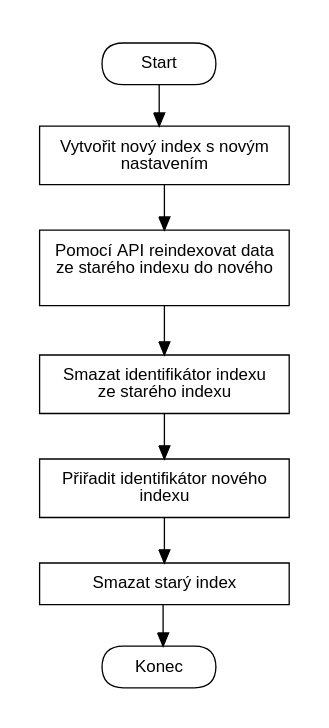
\includegraphics[width=5cm]{obrazky/proces_reindexace_na_urovni_es}\hfill
			\caption{Ukázka procesu hromadné reindexace dat na úrovni Elasticsearch. Zdroj: [autor]}
		\end{figure}

		Druhým složitějším a časově náročnějším způsobem, který umožňuje indexovat kompletně nová data, je
		reindexace dat z primární databáze.
		Tento způsob obsahuje hromadné stažení entit z primární databáze, jejich transformaci do indexovatelných entit
		a hromadnou indexaci pomocí \ac{API}.
		Tento proces je zdlouhavý, právě kvůli nutnosti přesunutí dat mezi dvěma kompletně oddělenými systémy.

		\begin{figure}[H]
			\centering
			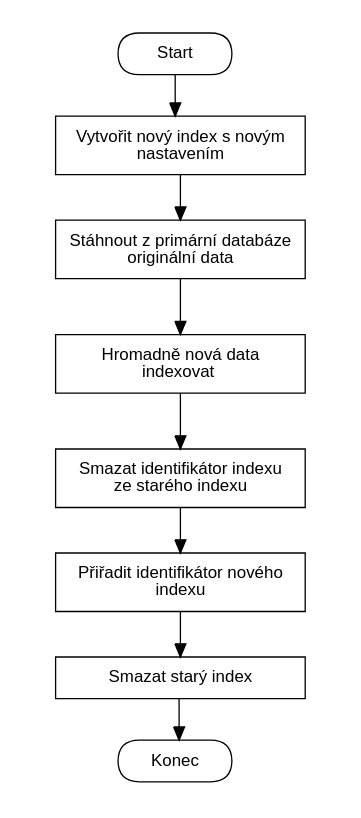
\includegraphics[width=5cm]{obrazky/proces_reindexace_z_db}\hfill
			\caption{Ukázka procesu hromadné reindexace nových dat z primární databáze. Zdroj: [autor]}
		\end{figure}

		Každý index svou spravující třídu, která obsahuje napojení na korektní index v databázi a jeho nastavení.

		\subsubsection{Nastavení aplikace}

		Nedílnou součástí větší aplikace jsou rozdílná nastavená každého provozního prostředí.
		Nastavení každé aplikace je vysoce individuální a záleží čistě na požadavcích aplikace.
		U většiny aplikací se nachází alespoň nastavení připojení k primární databázi, která je pro každého prostředí
		odlišná, aby nedocházelo k poškození dat (např.: mezi vývojovým a produkčním prostředím).

		Tato nastavení musí být dostupná v aplikace, a je tak nutné definovat jak se budou nastavená zapisovat a jak se
		zpřístupní kódu.
		V případě Java aplikací se často využívá "properties" souborů, které obsahují nastavení v podobě klíč-hodnota.
		V modernějších aplikacích postavených na frameworku Spring se tento formát postupně nahrazuje flexibilnějším
		\ac{YAML} jazykem, jenž umožňuje lépe definovat celé objekty a hodnoty jejich atributů podobně.

		\begin{lstlisting}[caption={Ukázka části nastavení aplikace v YAML konfiguračním souboru. Zdroj: [autor]}]
accounts:
	deletion:
		process-accounts-deletion-requests-every: 300
		delete-account-after: 180
	subscription:
		process-expiration-every: 60
		\end{lstlisting}

		Spring tyto soubory umí zpracovat a poskytnout jednotlivé hodnoty atributů programátorovi.
		Nicméně používání tohoto způsobu pro získaní nastavení napříč aplikací je náchylné k chybovosti a
		zesložiťuje úpravu struktury nastavení.

		Proto byla vytvořena tenká abstrakce nad Springovými nástroji vystavující jasně definovavé třídy a jejich atributy
		reflektující nastavení celé aplikace.
		Implementace zahrnovala připravení datového modelu a načítače hodnot z \ac{YAML} souborů.

		\begin{figure}[H]
			\centering
			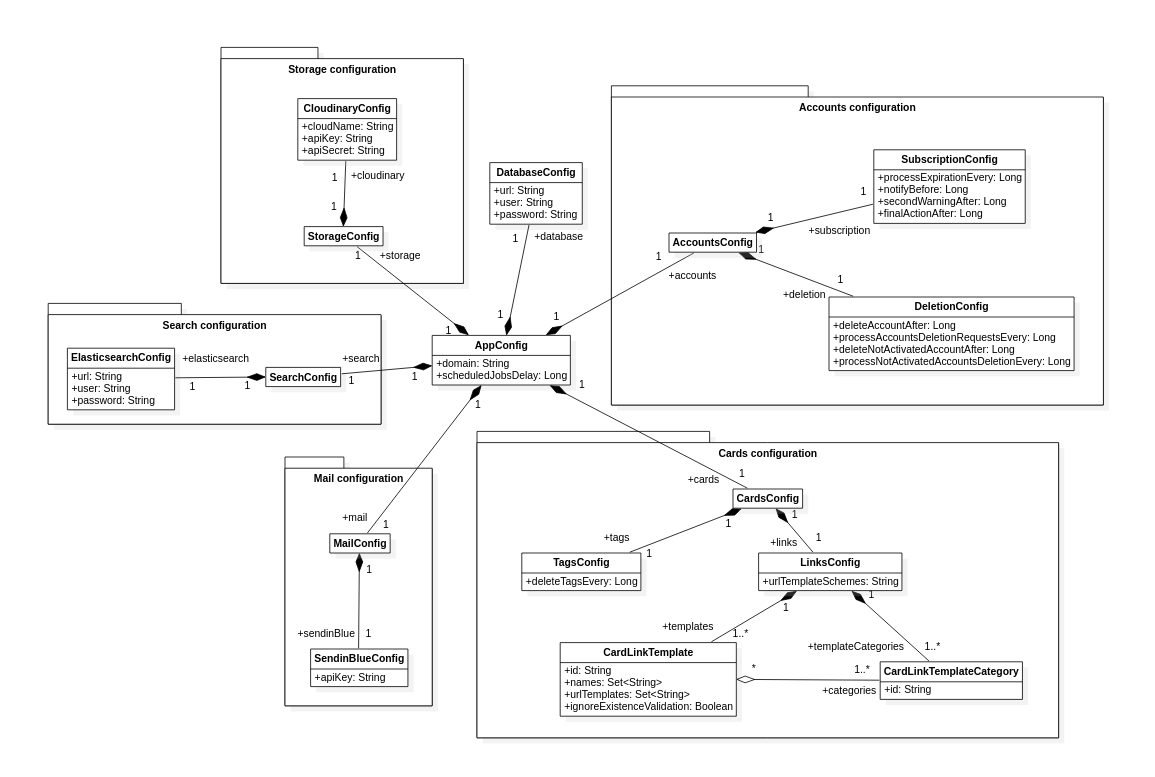
\includegraphics[width=\linewidth]{obrazky/datovy_model_nastaveni_aplikace}\hfill
			\caption{Ukázka datového modelu nastavení aplikace.}
		\end{figure}

		\subsubsection{Šablony odkazů sítí}

		Aby bylo možné uživatelům poskytnou komfort v podobě předdefinovaných sociálních sítí společně s validací \ac{URL} adres,
		bylo potřeba vytvořit robustní systém.
		Proto byl vytvořen systém šablon, v němž každá šablona definuje vlastnosti jedné sítě.
		Každý konkrétní odkaz pak má přiřazenou jednu šablonu, na základě které je možné adresu validovat a
		zobrazit uživateli správnou ikonu a název sítě.
		Definice šablon jsou načítány z \ac{YAML} souboru v rámci celého nastavení aplikace.

			\paragraph{Šablony URL adres}

			Šablony \ac{URL} adres slouží pro specifikování vzoru povolených \ac{URL} adres dané sítě.
			Tím je zaručeno, že odkaz vede skutečně na ověřenou síť.
			Zároveň to umožňuje získat ID profilů z \ac{URL} adresy odkazu fulltextového
			vyhledávání karet.

			S pomocí speciálních vyhrazených sekvencí znaků je možné definovat poměrně velké množství kombinací
			šablon.
			Šablony jsou při načtení zanalyzovány a jsou z nich vytvořeny Regex výrazy.
			Regex je výrazový jazyk skládající se ze speciálních znaků definující pravidla porovnávání \cite{regex}.
			Díky tomu je možné jednoduše zjišťovat, jestli textové řetězce vyhovují nějakému výrazu.
			Systém momentálně podporuje sekvence \lstinline{*} a \lstinline!{userPart}!.
			Sekvence \lstinline{*} říká, že se na tomto místě může nacházet jakýkoliv znak, vyjma hostové části \ac{URL}
			adresy, kde se mohou pod touto sekvencí skrývat pouze písmena a pomlčky.
			Sekvence \lstinline!{userPart}! může obsahovat stejné znaky jako \lstinline{*} sekvence, avšak textové
			řetězec označené touto sekvencí mají speciální význam.
			Nachází se v něm totiž právě zmiňované profilové ID.
			Díky tomuto označení je pak systém schopen určit, kde se profilové ID nachází a vytáhnou jej.

			\begin{lstlisting}[caption={Ukázka šablon URL adres. Zdroj: [autor]}]
https://*.example.com/{userPart}
https://{userPart}.example.com
			\end{lstlisting}

			Systém obsahuje různé validace aplikované při analyzování šablon, aby se do aplikace nemohli načíst
			nevalidní šablony.
			Momentálně definovanými pravidly URL šablon jsou následující:
			\begin{itemize}
				\item právě jedna sekvence \lstinline{userPart},
				\item oddělovač mezi jednotlivými sekvencemi,
				\item šablona je po záměně sekvencí náhodnými slovy validní \ac{URL} adresa.
			\end{itemize}

			\paragraph{Validace odkazů}

			Standardní validace se skládá ze dvou hlavních částí.
			První část řeší, jestli \ac{URL} adresa odpovídá předpokládané \ac{URL} šabloně.
			Předpokládaná šablona je určena nadřazenou skupinou odkazů.
			Validátor se pak pokusí pro předanou adresu nalézt existující šablonu.
			Pokud je tento předpoklad splněn, a zároveň se má validovat existence adresy, přechází validátor do druhé části.
			Druhá část se zabývá validací existence \ac{URL} adresy, tedy, zda URL adresa odkazuje na nějakou existujicí
			webovou stránku.
			Toto se ověřuje simulováním \ac{HTTP} požadavku webového prohlížeče, a z odpovědi se zjistí, že buď stránka
			existuje, stránka neexistuje nebo \ac{URL} adresa přesměrovává na jinou stránku.
			V prvních dvou případech validace končí jasným výsledkem: validní, nevalidní.
			V tom posledním se proces opakuje s novou vrácenou \ac{URL} adresou.
			I u této adresy se kontroluje šablona a existence.
			Takto se proces opakuje do té doby, než validátor nedostane jasnou odpověď existence, nebo vyprší interně stanovený
			limit přesměrování.
			Limit byl zaveden, aby nemohlo dojít k potencionálnímu zacyklení validace.
			Je ale nastaven dostatečně vysoký, aby nedocházelo k předčasným selhání.

			\begin{figure}[H]
				\centering
				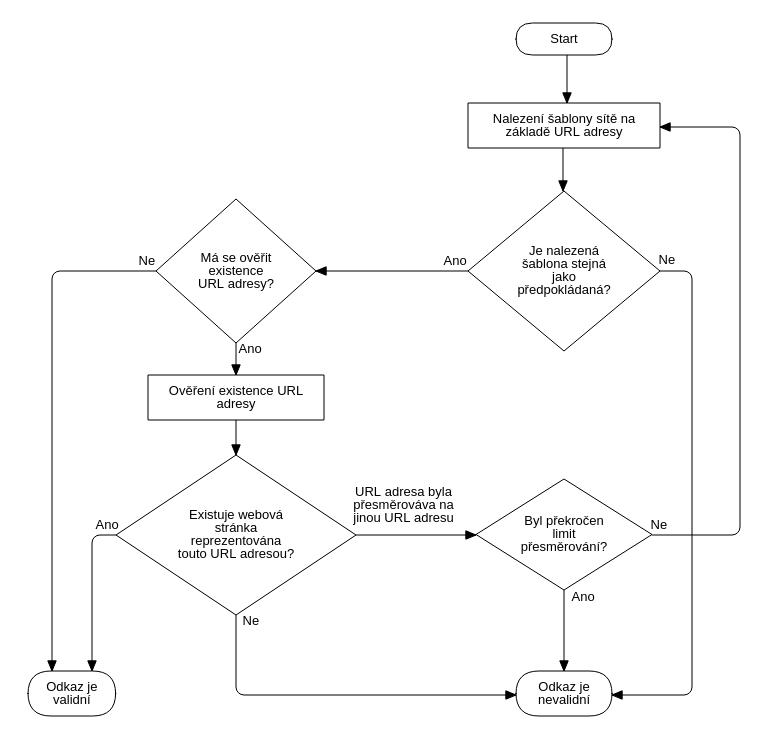
\includegraphics[width=\linewidth]{obrazky/proces_validace_odkazu}\hfill
				\caption{Proces validace URL adresy odkazu. Zdroj: [autor]}
			\end{figure}

			Bohužel ne u všech \ac{URL} adres lze validovat existenci.
			Některé stránky mají pokročilou ochranu proti škodlivým strojovým botům, které tento validátor označí za
			škodlivého bota.
			Byly provedeny optimalizace v podobě úpravy \ac{HTTP} hlaviček, aby se validace tvářila jako webový prohlížeč,
			a u některých stránek to skutečně pomohlo, jiné jsou ale pečlivější.
			Proto se zavedl příznak přímo do definice šablon, který tuto validaci existence vypíná.
			Naštěstí se jedná o nižší procenta stránek, a pro bezpečnost uživatelů je stěžejní pouze první část validace.

		\subsubsection{Prémiový plán a předplatné}

		Proces aktivace prémiového plánu začíná aktivováním platného kupónu.
		Na základě této aktivace je uživateli přiřazena speciální role a vytvořen nový popisný objekt předplatného
		obsahující datum expirace.
		Datum expirace je vypočítán z doby platnosti kupónu.
		Každý kupón definuje, po jakou dobu bude předplatné aktivní, a při aktivaci se tato doba přičte k aktuálnímu datu.
		V tuto chvíli uživatel může využívat všechny prémiové funkce.
		Pokud by v tuto chvíli uživatel aplikoval další kupón, datum expirace by se změnil podle nového kupónu.

		V případě placeného předplatného by objekt předplatného zprvu datum expirace neměl.
		Ta by se nastavila automaticky, až při neprovedené následující platbě.

		Systém tedy při vytváření a ukládání karet musí vždy validovat zda daná karta neobsahuje prémiový obsah.
		Pokud ano, musí zkontrolovat, zdali uživatel má příslušnou roli.
		V případě, že by neměl, je celý požadavek zaříznut a uživateli je vrácena chyba.

		Nejkomplikovanější částí celého systému je expirace předplatného.
		Problém spočívá v existenci prémiového obsahu.
		Pokud uživatel v době expirace nemá na svém účtu prémiový obsah, je situace jednoduchá a předplatné se zruší okamžitě.
		Pokud však uživatel v době expirace má na svém účtu prémiový obsah, je potřeba s těmito daty nějak naložit.
		Uživatel tak dostane tři možnosti.
		Tou nejjednodušší je upozornění ignorovat, a v takovém případě se po nějaké době všechny karty uživatele skryjí
		a veřejnost se na ně už nepodívá.
		Druhou možností je prémiový obsah pomocí speciálního formuláře odstranit, aby bylo možné zrušit předplatné.
		Poslední možností je prodloužení předplatného.
		V tomto případě uživateli všechen obsah zůstane a může prémiové funkce nadále využívat.

		Celý proces začíná nějakou dobou před expirací.
		Uživatel je dopředu emailem upozorněn na blížící se expiraci.
		Pokud uživatel do té doby nesmaže všechen prémiový obsah, v den expirace přijde druhý email s informací o
		proběhlé expiraci, a možnostmi, které uživatel může provést.
		Pokud bude uživatel ignorovat toto upozornění, během několika dní mu přijde druhé upozornění.
		V případě, že uživatel ignoruje i toto poslední varování, všechna data uživatele jsou během několika dní
		automaticky skryta.
		Uživateli už jen o skrytí dat přijde informativní email.

		Zvolený přístup se jeví jako dostatečně flexibilní a pokrývá všemožné scénáře požadované aplikací.

		\subsubsection{REST API}

		K zajištění komunikace mezi front-endovou \ac{GUI} aplikací a aplikací \ac{API} serveru, server
		vystavuje právě \ac{REST} \ac{API}.
		Díky němu je možné vytvářet, ukládat a získávat entity, a spouštět různé akce.

		\ac{REST} \ac{API} obecně pracuje s tzv. zdroji.
		Každý zdroj představuje jeden typ pojmenovatelné informace.
		Tím může být entita, obrázek, dokument, nebo třeba kolekce.
		Jednotlivé zdroje jsou pak vystaveny na přesně daných \ac{URL} adresách, a pomocí \ac{HTTP} metod (GET, POST, PUT...)
		je možné s těmito zdroji provádět operace.
		Operace jsou většinou následující: získání konkrétního zdroje nebo jeho kolekce, vytvoření nového zdroje nebo
		úprava již existujícího zdroje.
		Nejrozšířenějším jazykem pro popis zdrojů je \ac{JSON}, díky kterému je možné objekty aplikace jednoduše
		mapovat na \ac{JSON} dokumenty. \cite{restfulapi}

			\paragraph{Struktura API}

			Implementované \ac{API} v běžných scénářích (získání, vytvoření a úprava zdrojů) respektuje doporučovaná pravidla.
			Nicméně v krajních případech je potřeba provádět i jiné, většinou servisní, operace, které tyto pravidla porušují.
			Toto je však poměrně běžná praxe, a pokud takto není navržena větší část \ac{API}, nepředstavuje je to velký
			problém.

			Jak je možné vidět níže, \ac{API} pro uživatelské účty zahrnuje manipulaci s účtem přihlášeného uživatele a manipulaci
			s oblíbenými kartami.

			\begin{figure}[H]
				\centering
				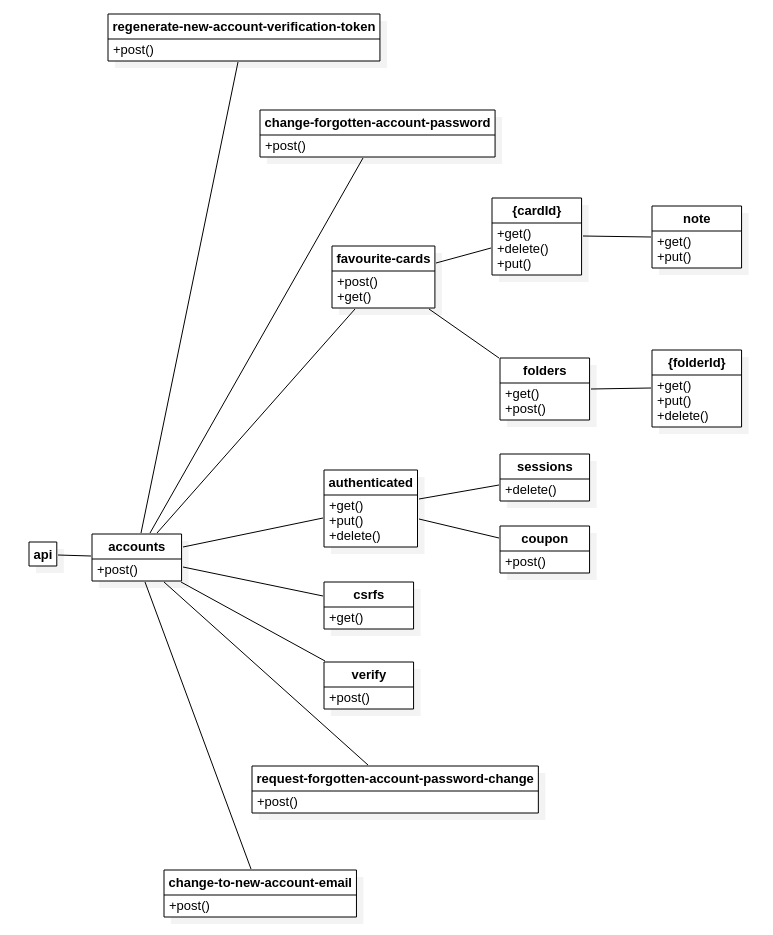
\includegraphics[width=\linewidth]{obrazky/api_model_ucty}\hfill
				\caption{Stromový přehled struktury API uživatelských účtů. Zdroj: [autor]}
			\end{figure}

			Nejpodstatnější \ac{API} se zabývá manipulací karet, a zároveň umožňuje získávat i další podřzené entity.
			Mimo to nabízí i pomocné operace pro manipulaci s display ID.

			\begin{figure}[H]
				\centering
				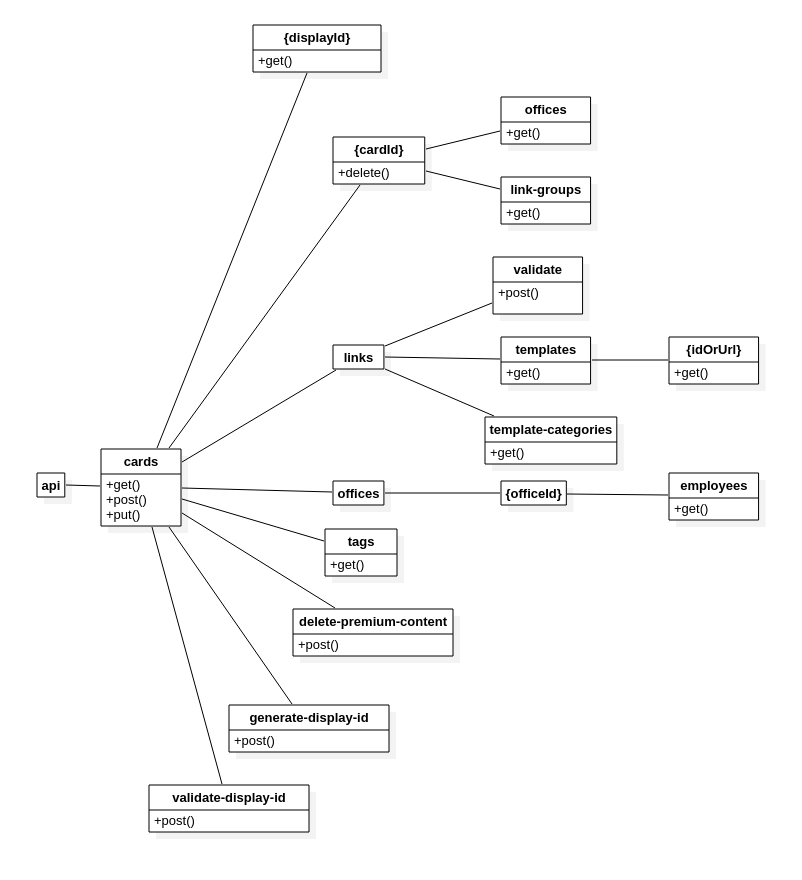
\includegraphics[width=\linewidth]{obrazky/api_model_karty}\hfill
				\caption{Stromový přehled struktury API karet. Zdroj: [autor]}
			\end{figure}

			\ac{API} úložiště momentálně umožňuje pouze soubory nahrávat, protože systém pracuje pouze s věřejnými soubory, které
			lze získat přímo z Cloudinary serverů.

			\begin{figure}[H]
				\centering
				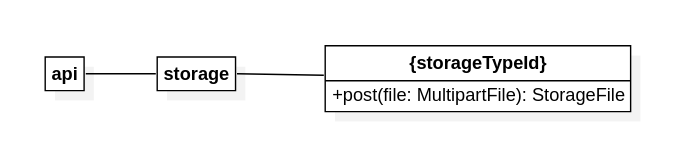
\includegraphics[width=8cm]{obrazky/api_model_uloziste}\hfill
				\caption{Stromový přehled struktury API uložiště. Zdroj: [autor]}
			\end{figure}

			Pro přehlednost vyhledávání karet a míst existuje separátní vyhledávací \ac{API}.

			\begin{figure}[H]
				\centering
				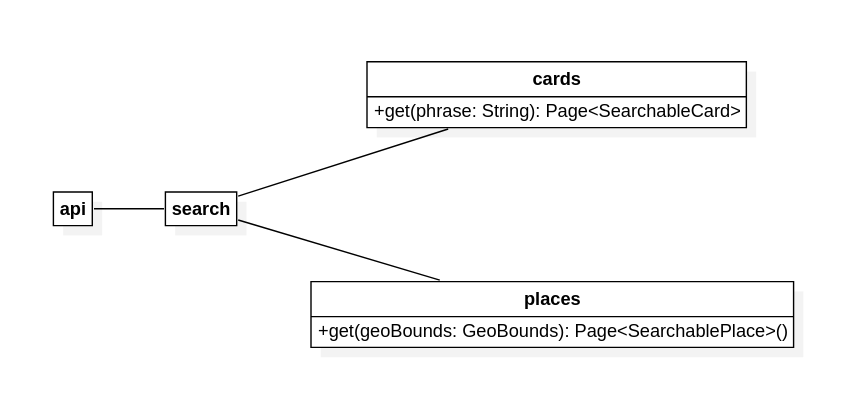
\includegraphics[width=8cm]{obrazky/api_model_vyhledavani}\hfill
				\caption{Stromový přehled struktury API vyhledávání karet. Zdroj: [autor]}
			\end{figure}

			Aplikace také nabízí interní administraci pro správce.
			Proto vzniklo i \ac{API} pro spouštění servisních operací a k správě zákulisních zdrojů (např.: kupóny).

			\begin{figure}[H]
				\centering
				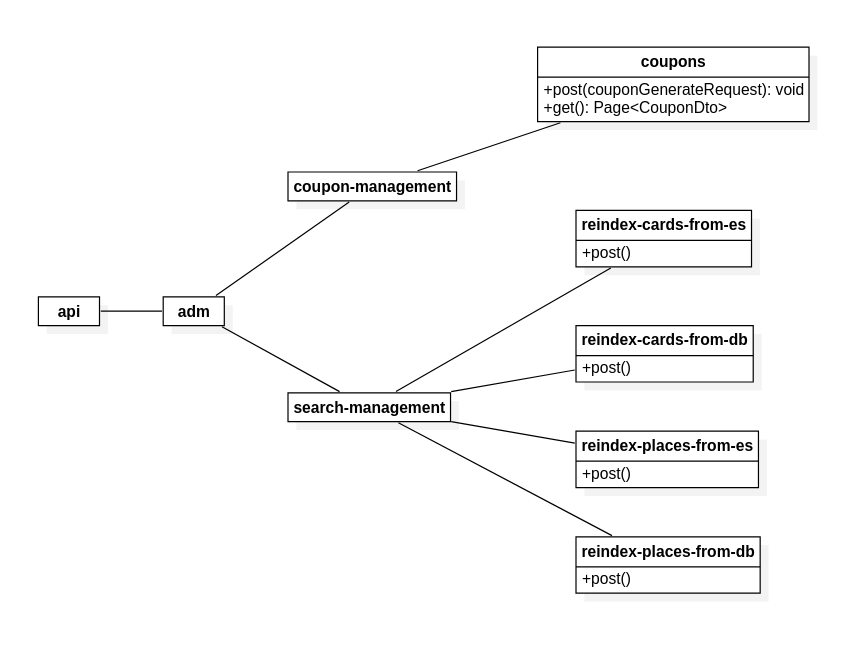
\includegraphics[width=\linewidth]{obrazky/api_model_adm}\hfill
				\caption{Stromový přehled struktury API operací administrace. Zdroj: [autor]}
			\end{figure}

			\paragraph{Objekty pro přenos dat}

			V rámci komunikace mezi konzumentem \ac{API} a serverem je nezbytné přenášet objekty reprezentující data
			aplikace.
			K tomu by šlo využít přímo doménových tříd.
			Bohužel některé tyto třídy obsahují data, která by se neměla dostat mimo server.
			Nejtypičtějšími takovými daty jsou hesla uživatelů.
			Někdy je také nezbytné poskytnout agregované atributy, které však nemají své místo v originálních datech.
			Právě z těchto důvodů \ac{API} využívá tzv. objektů pro přenost dat neboli \ac{DTO}.
			Tyto datové objekty slouží obecně pro přenos daty mezi procesy.
			V tomto případě přenáší data mezi \ac{API} serverem a front-endovou aplikací.

			\ac{API} tak na venek pracuje pouze s \ac{DTO} objekty, které reflektují doménové objekty.
			Speciálním případem jsou \ac{DTO} objekty jenž slouží pouze pro jednorázové předání dat.
			Většinou se používají pro specifikování požadavků front-endové aplikace na zvolenou operaci, nebo jako
			objekty nesoucí výsledek nějaké operace.

			Pro transformaci mezi doménovými objekty a \ac{DTO} objekty vznikla jednoduchá podpora pro standardizovanou
			a centralizovanou transformaci.
			Slouží k tomu továrnové třídy dědící z obecného rozhraní, v němž se nacházejí metody pro transformaci z doménového
			objektu na \ac{DTO} objekt a naopak.

			\begin{lstlisting}[language=Java, caption={Ukázka obecného rozhraní třídy pro transformaci mezi doménovými objekty a DTO objekty. Zdroj: [autor]}]
public interface DtoFactory<E, D> {
    D createDto(E entity);
    E updateEntity(E originalEntity, D dto);
}
			\end{lstlisting}

			Transformace z \ac{DTO} objektu na doménový objekt je specifická v tom, že pro transformaci používá zároveň
			i originální doménový objekt z databáze.
			Díky tomu je možné zajistit, že výsledný objekt bude mít změněné pouze ty atributy, u nichž je to povolené.

			Rozhraní továrny je generické, a proto pro každá doménová entita má vlastní implementaci.

			\paragraph{Zabezpečení}

			Zabezpečení je velmi důležitou součástí aplikace pro znemožnění zneužití dat útočníky.
			Je nezbytné zajistit, aby se neoprávnění uživatelé nedostali k datům, které jim nepřísluší, a aby nemohli
			poškodit cizí data.
			Těmito problémy se zabývá především společnost OWASP poskytující kvalitní materiály o bezpečnosti programátorům.
			Avšak řešit všechny existující problémy svépomocí by zabralo spoustu času, a bez dlouholetých znalostí v
			oblasti bezpečnosti, by implementovaný systém nemusel být ani správně zabezpečený.

			Naštěstí framework Spring zahrnuje i knihovnu Spring Security.
			Tato knihovna jednak automaticky zajišťuje doporučené bezpečnostní praktiky, a jednak poskytuje programátorovi
			nástroje pro tvorbu přihlašování a práv uživatelů.
			Programátor si navíc tyto nástroje může relativně snadno rozšířit nebo implementovat vlastní.

			Specificky pro tuto aplikaci bylo definováno jaké \ac{URL} adresy \ac{API} vyžadují přihlášení a specifické
			role, a výchozí přihlašovací proces byl rozšířen o externí poskytovatele a vlastní správu účtů.

			\begin{lstlisting}[language=Java, caption={Ukázka části nastavení zabezpečení API pomocí knihovny Spring Security. Zdroj: [autor]}]
@Override
protected void configure(HttpSecurity http) throws Exception {
        http
            .mvcMatchers(HttpMethod.GET, "/api/search/cards").permitAll()
            .mvcMatchers(HttpMethod.GET, "/api/search/places").permitAll()
            .mvcMatchers("/api/adm/**").hasRole("ADMIN")
            .mvcMatchers("/api/**").authenticated()
            .anyRequest().denyAll()
        /* ... */
}
			\end{lstlisting}

			\paragraph{Přihlašování}

			Korektní implementace procesu přihlašování je pro aplikaci využívající uživatelské účty stěžejní.
			Zabraňuje neoprávněným uživatelům vydávat se za jiné uživatele.
			Standardním, dlouhá léta využívaným, přístupem je ověření kombinace emailové adresy/uživatelského jména
			a hesla.
			U tohoto přístupu kombinaci ověřuje přímo aplikace.
			Druhým, stále více používaným, přístupem je přihlašování pomocí třetích stran.
			Při tomto přístupu aplikace deleguje přihlašování na jiného poskytovatele uživatelských účtů, který následně
			vrátí aplikaci informace o přihlášeném uživateli.
			Aplikace se tak nemusí starat o ověřování hesla a podobně.
			Takovýchto poskytovatelů existuje celá řada, což přispělo vzniku standardu OAuth2, který standardizuje celý proces
			komunikace mezi aplikací a poskytovatelem.
			Díky tomu není potřeba pro každého poskytovatele implementovat odlišný proces.

			Aby měli uživatelé volnost při výběru, jakým způsobem se chtějí přihlašovat, byly do této aplikace implementovány
			oba způsoby.
			Uživatel se tak může přihlásit a zaregistrovat, buď pomocí běžné kombinace emailové adresy a hesla, nebo pomocí
			některých z poskytovatelů.
			Momentálně jsou připraveni nejvyužívanější poskytovatelé Google, Github a Facebook, nicméně rozšíření o
			další poskytovatele nepředstavuje příliš práce.
			Zaregistrovaný uživatel si pak může ke svému účtu připojit i další způsoby, tedy, pokud se zaregistroval emailovou
			adresou, může si připojit některého z poskytovatelů a obráceně.
			Díky tomu si uživatel může při každém přihlášení vybrat, jakým způsobem se přihlásí.

			Druhým řešeným problémem je, jak verifikovat přihlášeného uživatele při každém následujícím \ac{HTTP} požadavku na server,
			aniž by musel uživatel pokaždé zadávat přihlašovací údaje.
			Aplikace na serveru může buď udržovat v paměti sezení každého uživatele nebo vygenerovat uživateli token
			obsahující informace o uživateli.

			V případě, že aplikace využívá sezení, je na serveru spravován objekt s informacemi o přihlášeném uživateli.
			Uživatel pomocí webového prohlížeče pak pouze předává ID daného sezení.
			Server má tak plnou kontrolu nad daným sezením.
			Bohužel server musí zajistit opatření proti krádeži těchto ID.

			Alternativou je vygenerování tokenu obsahující uživatelské informace.
			Tento token je následně předán klientovi, a ten musí zaručit předání vygenerovaného tokenu severu.
			Tento způsob je převážně využíván pro komunikaci mezi servery, avšak začíná se používat i v aplikacích, kde
			je aplikace rozdělena na \ac{GUI} část a \ac{API} část.
			Díky tomuto přístupu server nemusí udržovat sezení přihlášených uživatelů.
			Tím že server nemá token pod svojí správou, není snadné takový token označit jako neplatný, třeba v případě odhlášení.
			To jde řešit například ukládáním tokenů do databáze, nicméně správa tokenů se pak částečně přenáší zpět
			na server, a výhody nezávislosti na serveru mizí.
			Řešení se tak přibližuje přístupu se sezeními, avšak za cenu složitější implementace.

			V případě této aplikace proběhl experiment s druhým typem ověřování, posléze se ale ukázalo, že
			řešení je zbytečně složité a ne úplně spolehlivé.
			Přihlašování bylo tedy přepracováno na řešení se sezeními, které má již knihovna Spring Security v základu
			vyřešené, což neplatilo o předchozím přístupu.
			Díky tomu se celý proces zjednodušil a delegoval se na externí knihovnu, na které pracují experti v oboru.
			Bonusem bylo zjednodušení implementace přihlašování pomocí poskytovatelů třetích stran, protože pro tyto scénáře
			má knihovna Spring Security připravenou podporu.

			Jediným problémem bylo spojení interních uživatelských účtů a OAuth2 účtů.
			Spring Security totiž pro každý způsob využívá jiné objekty.
			Proto byl proces připravený knihovnou rozšířen o vlastní zakončení.
			Toto zakončení je vyvoláno knihovnou po úspěšném přihlášení poskytovatelem, a dává možnost provést vlastní operace nad
			přihlášeným uživatelem než se odpověď dostane ke koncovému uživateli.
			Proces řeší i registraci nového uživatele, protože OAuth2 nerozlišuje mezi novým a existujícím uživatelem.
			OAuth2 pouze zajišťuje poskytnutí uživatelských dat.

			\begin{figure}[H]
				\centering
				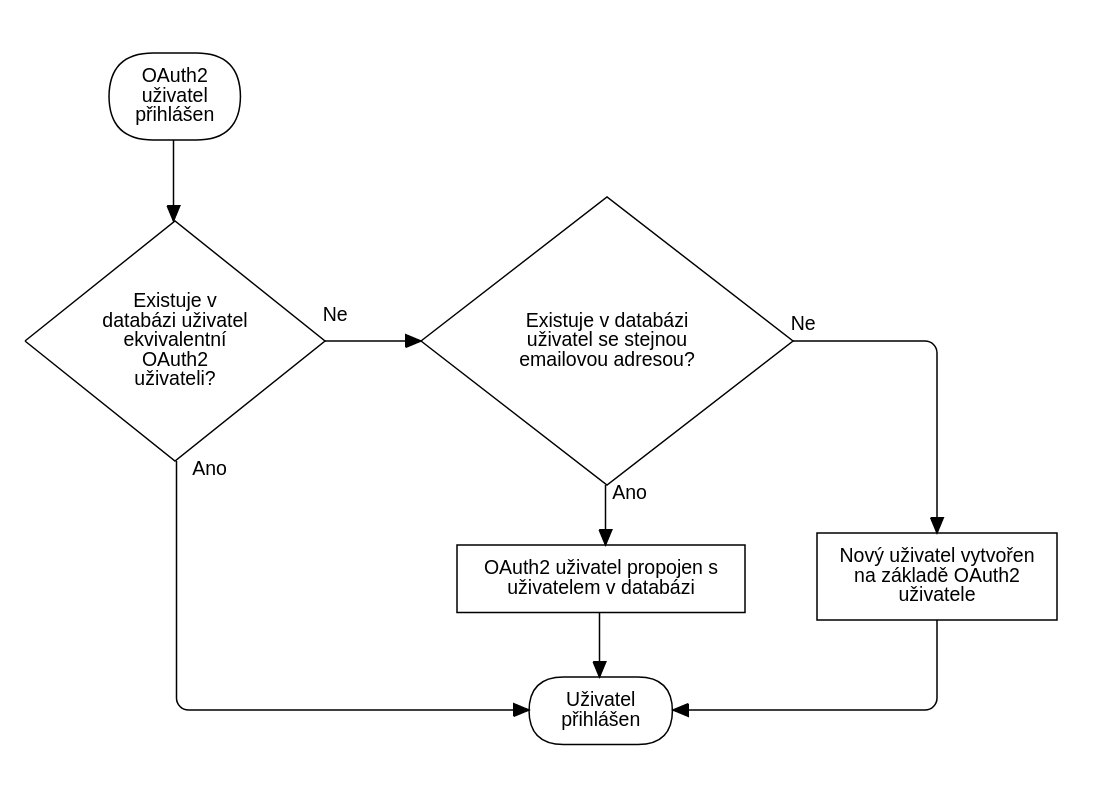
\includegraphics[width=\linewidth]{obrazky/proces_prihlaseni_oauth2}\hfill
				\caption{Proces zpracování přihlášeného OAuth2 uživatele a transformace na interního uživatele. Zdroj: [autor]}
			\end{figure}

		\subsubsection{Automatizované testování}

		Automatizované testování umožňuje kód aplikace otestovat ještě před samotným spuštěním a testovat
		kód průběžně při úpravách a rozšiřováních.
		Díky tomuto testování je možné předejít velkému množství logických chyb, již v počátku implementace.

		Způsobů testování je více.
		Tato aplikace využívá unit testování a integračního testování.
		Unit testování izolovaně ověřuje předpokládané chování komponent systému vlivu
		ostatních komponent \cite{unit_testing}.
		Opakem je integrační testování, jenž ověřuje souhru více komponent najednou \cite{integration_testing}.

		Služební třídy a pomocné třídy provádějící nějaké transformace (\ac{DTO} továrny, analyzátor šablon odkazů...)
		jsou testovány izolovaně pomocí unit testů.
		Pro každou metodu každé třídy je připraveno několik testů ověřující různé scénáře: běžné chování při různých datech,
		chování při chybných datech a podobně.
		Hlavní knihovnou zpřístupňující nástroje pro spouštění testů a ověřování výsledků je JUnit.
		Aby bylo možné třídy testovat izolovaně, je potřeba simulovat chování ostatních komponent, se kterými testovaná
		třída komunikuje.
		K tomu je využita knihovna Mockito, která zároveň umožňuje zkoumat proběhlé interakce, a na základě toho vyhodnocovat testy.

		\begin{lstlisting}[language=Java, caption={Testu ověřující, že služba štítků vrací správné nejvyužívanější štítky z nasimulovaného repozitáře. Zdroj: [autor]}]
@Test
public void getMostUsedTags_ExpectedFoundCorrectOnes() {
	when(cardTagDaoMock.findMostUsed(3)).thenReturn(Set.of(
			new CardTag(null, "dev"),
			new CardTag(null, "nature"),
			new CardTag(null, "tech")
	));
	assertEquals(
			Set.of("dev", "nature", "tech"),
			cardTagService.getMostUsedTags(3)
	);
}
		\end{lstlisting}

		Třídy repozitářů a třídy poskytující \ac{REST} \ac{API} jsou spíše integračními testy spojujícími více
		komponent k zajištění výsledků.

		Při testování repozitářů je potřeba testovat \ac{SQL} dotazy oproti reálné databázi s daty.
		K spuštění takových testů je tedy potřeba běžící testovací databáze s připravenými testovacími daty.
		Ta jsou do databáze nahrávána před každým testem a mazána po každém testu.
		Tím je zaručena izolovanost jednotlivých testů, aby nedocházelo k mylným výsledkům.

		Testy \ac{REST} \ac{API} jsou kombinací integračních a unit testů.
		Knihovna Spring poskytuje nástroje pro volání \ac{API} skrze \ac{URL} adresy, které simulují reálnou komunikaci
		s \ac{API}.
		Napojení na služební třídy je ale řešeno simulací, aby nebylo nutné zprovozňovat všechny části
		aplikace.

		\begin{lstlisting}[language=Java, caption={Ukázka testu volání API validující odkaz. Zdroj: [autor]}]
@Test
@WithMockUser
public void validateLink_InvalidLink_ExpectedFalse() {
	/* ... */
	mockMvc.perform(post("/api/cards/links/validate")
					.accept(MediaType.APPLICATION_JSON)
					.contentType(MediaType.APPLICATION_JSON)
					.content(objectMapper.writeValueAsString(requestBody))
					.with(csrf()))
			.andDo(print())
			.andExpect(status().isOk())
			.andExpect(content().contentType(MediaType.APPLICATION_JSON))
			.andExpect(content().json(objectMapper.writeValueAsString(expectedResponseBody)));
}
		\end{lstlisting}

	\subsection{Implementace front-endové aplikace}

	Front-endová aplikace zpřístupňující \ac{GUI} koncovým uživatelům byla postavena na frameworku
	Nuxt obalující knihovnu Vue.
	Díky tomu je zajištěna reaktivnost komponent a prvotní vykreslení stránek na serveru.
	Zaměření tak padlo na konkrétní problémy řešené domény.

		\subsubsection{Komunikace s API serverem}

		Prvním stavebním kamenem je možnost komunikovat s vyvinutým \ac{API}.
		Opět existuje spousta ověřených knihoven řešící problémy komunikace.
		Nuxt přichází se svou vlastní, která má jednoduché \ac{API}, a proto byla zvolena.
		Díky integraci s Nuxt frameworkem bylo možné jednoduše centralizovaně přednastavit knihovnu pro všechna volání \ac{API}.
		Hlavní takovou konfigurací byla správa chyb z volání \ac{API}.
		Ta řeší obecné chyby, jako je nepřihlášený uživatel nebo nedostatečná práva uživatele.
		Zároveň řeší, aby v každém požadavku byl zahrnut platný \ac{CSRF} token.
		\ac{CSRF} token zabraňuje útočníkům provádět operace pod účtem jiného uživatele pomocí podvodných stránek \cite{csrf}.
		Token je poskytován \ac{API} serverem na vyžádání.
		Front-endová aplikace však musí zaručit jeho získání a následné uložení pro další požadavky.
		Předání tokenu zpět \ac{API} serveru je zajištěno přidáním tokenu před odesláním \ac{HTTP} požadavku do speciální hlavičky.
		Pokud token v aplikaci ještě neexistuje, je odeslán paralelní požadavek na \ac{API} server pro vygenerování tokenu.

		\begin{lstlisting}[caption={Ukázka vložení CSRF tokenu do každého požadavku putujícího na API server. Zdroj: [autor]}]
$http.onRequest(async (request) => {
	if (!csrfAllowedMethods.includes(request.method)) {
		await addCsrfTokenToRequest(store, $http, request)
	}
})
		\end{lstlisting}

		\subsubsection{Centrální zdroj informací}

		Dalším důležitým stavebním prvkem je tzv. centrální zdroj informací.
		Ten představuje centralizované místo pro ukládání a získávání dočasných dat napříč celou aplikací.
		Je zde možné například uložit informace o přihlášeném uživateli nebo výše zmíněný \ac{CSRF} token.
		K tomu slouží knihovna Vuex řešící uchování dat a záznam změn v čase.
		Díky ní je pak uživatelský účet jednoduše přístupný ze všech komponent bez nutnosti opakovaného provolávání
		\ac{API} serveru.

		\subsubsection{Lokalizace textů}

		Lokalizace textů se zabývá zobrazováním textů prvků \ac{UI} v konkrétním jazyce uživatele.
		Díky tomu různí uživatelé mluvící odlišnými jazyky mohou bez problému aplikaci využívat v jejich nativním jazyce.

		Tuto problematiku řeší například knihovna i18n od tvůrců frameworku Nuxt.
		Konkrétně zajišťuje nahrazování klíčů konkrétními texty v komponentech, a automatické přepínání použitého jazyka
		podle webové prohlížeče.

		Problém ale nastal při tvorbě informačních stránek (nápověda, podmínky použití...).
		U těchto stránek je obsah zapsán jako jeden velký \ac{HTML} soubor pro podporu formátování, nikoli
		jako dílčí texty.
		Knihovna však očekává všechny texty zapsané v jednom \ac{JSON} dokumentu.
		Do těchto dokumentů bylo potřeba nějakým způsobem vložit i ty \ac{HTML} dokumenty.
		Z tohoto důvodu pro každý jazyk vznikl \ac{JS} soubor, který posbírá všechny překladové materiály a poskládá z nich
		výsledný \ac{JSON} dokument.

		\subsubsection{Validace formulářových polí}

		Validace uživatelsky vložených dat je důležitá především pro zaručení správnosti uložených dat.
		Ne všichni uživatelé jsou však podvodníci chtějící poškodit data.
		Většina uživatelů zadává očekávaná data, nicméně je velká pravděpodobnost, že se nějaký uživatel omylem upíše
		a udělá nechtěnou chybu.
		Proto je dobré v rámci kvalitního \ac{UX} poskytnout uživatelům rychlou a cílenou zpětnou vazbu o chybně zadaných
		datech.

		\begin{figure}[H]
			\centering
			
\includegraphics[width=8cm]{obrazky/nevalidni_pole_formulare}\hfill
			\caption{Ukázka pole formuláře s textem v nevalidním formátu. Zdroj: [autor]}
		\end{figure}

		Pomocí knihovny Vuelidate bylo implementováno zobrazování chyb přímo v konkrétních polích hned,
		jakmile uživatel vyplní dané pole.
		Knihovna řeší celý mechanismus validace hodnot polí a poskytování výpisu všech chyb ve formuláři.
		Zároveň přichází s obecnými validátory, ale programátor může implementovat i vlastní.
		Toho bylo využito především u validace \ac{URL} adres odkazů na sociální síťě, u nichž je potřeba se dotázat \ac{API},
		které adresu zvaliduje.

		\begin{lstlisting}[caption={Ukázka implementace vlastního validátoru využívající API k validaci hodnoty. Zdroj: [autor]}]
export const displayId = function (cardId) {
	return async function (displayId) {
		const requestBody = { cardId, displayId }
		try {
	  		return (await this.$http.$post('cards/validate-display-id', requestBody)).valid
		} catch (e) {
		    this.$notifyError()
		}
	}
}
		\end{lstlisting}

		S připravenými dílčími validátory je pak možné definovat pravidla pro jednotlivá pole ve formulářích.
		Tato pravidla jsou následně aplikována na jednotlivá pole, která sledují změny hodnot.
		Díky reaktivnosti Vue je pak možné chybu zobrazit hned, jakmile vznikne.
		Při odeslání formuláře je validace provedena ještě jednou, a buď je formulář odeslán nebo je
		zobrazena chyba.
		V případě běžných uživatelů by se tedy na server vůbec chybná data neměla dostat.

		\subsubsection{Upozornění v UI}

		Pokud v aplikaci vznikne nějaká událost (chyba, úspěšnost operace...), je nutné o tom informovat uživatele.
		To je v tomto případě vyřešeno vyskakujícími upozorněnými po vzoru mobilních operačních
		systémech.
		Tento způsob je výhodný v tom, že uživatel si upozornění všimne ať už je kdekoliv na stránce.
		Zároveň při přechodu mezi modálními okny se upozornění neztrácí.

		\begin{figure}[H]
			\centering
			
\includegraphics[width=6cm]{obrazky/upozorneni_chyba}\hfill
			\caption{Ukázka upozornění na chybu vzniklou špatnými přihlašovacími údaji. Zdroj: [autor]}
		\end{figure}

		K implementaci upozornění byla využita knihovna \url{https://www.npmjs.com/package/vue-notification}{Vue.js notifications}
		poskytující dostatečnou volnost přizpůsobení vzhledu a chování, oproti ostatním podobným knihovnám.
		Je navíc na míru tvořena pro knihovnou Vue.
		Knihovna poskytuje jednoduché \ac{API} pro vystavování upozornění pomocí specifikování typu zprávy (chyba, úspěch, info...) a
		samotné zprávy.
		Pro velkou aplikaci, kde je nutné na spoustě místech taková upozornění vystavovat, je nevhodné pokaždé duplikovat
		celou specifikaci upozornění.
		Stejně jako komponenty i upozornění využívají překladových textů.
		Tato kombinace tak značně zvyšuje riziko chybovosti kódu.
		Vznikla proto jednoduchá abstrakce zpřístupňující pomocné metody, které jsou dostupné celou aplikací.
		Pro každý používaný typ zprávy (chyba, úspěch, info) existuje právě jedna metoda vyžadující pouze klíč překladového textu.
		Malou výjimkou jsou chybové zprávy, kde existují dvě metody: jedna s možností vložení vlastního textu, druhá
		zobrazující generickou chybu.

		\begin{lstlisting}[caption={Implementované pomocné metody pro vystavení různých typů upozornění. Zdroj: [autor]}]
this.$notifySuccess('general.success.added')
this.$notifyInfo('general.info.linkCopied')
this.$notifyError('general.error.invalidData')
this.$notifyError()
		\end{lstlisting}

	\subsection{Příprava pro produkční provoz}

	Tím že celá aplikace poběží v orchestračním systému Kubernetes, je nutné zprovoznit obě aplikace v Docker kontejnerech.
	Následně nakonfigurovat Kubernetes, aby sám aplikace spustil a navázal mezi nimi spojení.

		\subsubsection{Příprava Docker image}

		Docker image je šablona, podle které se automatizovaně vytvářejí běžící kontejnery s aplikacemi.
		Pro \ac{API} server aplikaci a front-endovou aplikaci je nutné tedy připravit separátní Docker image.
		K tomu poslouží speciální soubor zvaný Dockerfile, sloužící jako předloha pro vytvoření Docker image.
		Dockerfile obsahuje všechny příkazy potřebné pro spuštění aplikace \cite{dockerfile_reference}.

		Součástí nadstavby Spring frameworku Spring Boot je možné automatizovaně Docker image vytvořit bez manuální tvorby
		Dockerfilu.
		Spring Boot tedy zajistí vytvoření optimalizovaného Docker image celé aplikace.

		V případě front-endové aplikace tato podpora není a bylo nutné Dockerfile připravit ručně.
		Nicméně příprava front-endové aplikace pro provoz v Docker kontejneru byla jednodušší, než by byla příprava \ac{API}
		serverové aplikace.
		Dockerfile obsahuje příkazy podobné tomu, jak se aplikace spouští pro lokální vývoj.
		Dockerfile nejdříve vytvoří cílový adresář pro aplikaci, následně nainstaluje potřebné systémové aplikace pro sestavení
		a běh aplikace.
		Nakonec aplikaci sestaví do vytvořeného adresáře a spustí na portu \lstinline{3000}.

		\begin{lstlisting}[caption={Dockerfile spouštějící front-endovou aplikaci v Dockeru. Zdroj: [autor]}]
FROM node:14.17.6-alpine

RUN mkdir -p /usr/src/netreachme-web-app
WORKDIR /usr/src/netreachme-web-app

RUN apk update && apk upgrade
RUN apk add git

COPY . /usr/src/netreachme-web-app/
RUN npm install yarn
RUN yarn install
RUN yarn build

EXPOSE 3000

ENV NUXT_HOST=0.0.0.0
ENV NUXT_PORT=3000

ENTRYPOINT yarn start --dotenv=.env.$ENV
		\end{lstlisting}

		\subsubsection{Nastavení Kubernetes}

		Na základě připravených Docker imagí pro obě aplikace byl zprovozněn systém Kubernetes.
		V systému se kromě implementovaných aplikací nachází i webový server nginx a databázový systém Elasticsearch.
		Jediný databázový systém PostgreSQL je provozován samostatně poskytovatelem DigitalOcean.
		Není tak nutné se starat o ruční zálohovaní nebo výpadky.

		\begin{figure}[H]
			\centering
			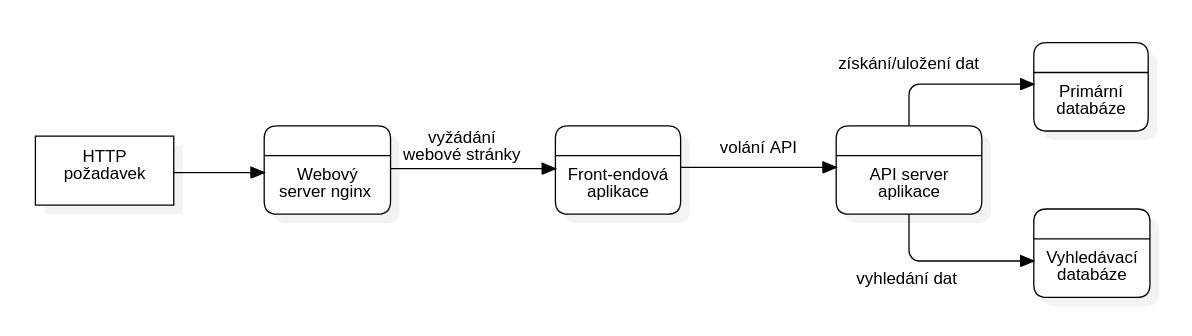
\includegraphics[width=\linewidth]{obrazky/architektura_produkce}\hfill
			\caption{Ukázka putování HTTP požadavku infrastrukturou. Zdroj: [autor]}
		\end{figure}

		Webový server slouží jako vstupní brána do celého systému a poskytuje nástroje pro zabezpěčení požadavků.
		Zároveň zahazuje neplatné požadavky ještě dřív, než by mohli způsobit škody v samotných aplikacích.
		Následně platné požadavky deleguje na serverovou část front-endové aplikace s požadavkem na poskytnutí webových stránek.
		V případě, že jsou vyžadována data z API serveru, front-endová aplikace část požadavku deleguje právě na \ac{API}.
		\ac{API} server si navíc data může vyžádat z primární databáze nebo vyhledávací databáze.
		Zpracovaný požadavek se nakonec vrací uživateli, opět skrze nginx.

		Obě aplikace a server nginx jsou nakonfigurované jako Deploymenty, jediný Elasticsearch je nastaven jako StatefulSet.
		Deployment je entita Kubernetes systému popisující, jak bude aplikace spuštěna \cite{deployements}.
		Deploymenty se používají v případě, kdy aplikace neudržuje důležitá data, o která by se v případě vypnutí přišlo
		\cite{deployements}.
		StatefulSety jsou jakousi nadstavbou nad Deploymenty, a zaručují udržení stavů spuštěných aplikací. \cite{statefulsets}.
		Právě z těchto důvodů mohou být implementované aplikace spuštěné jednoduššími Deploymenty, protože všechna důležitá
		data ukládají do PostgreSQL.
		Elasticsearch databáze je naproti tomu sama zdrojem dat a není vhodné, aby docházelo k jejímu vypínání.

		O finální spuštění takto nakonfigurovaného systému a vytvoření SSL certifikátů se stará poskytovatel; v tomto případě DigitalOcean.
		V tomto momentě jsou obě aplikace spuštěny a připraveny zpracovávat uživatelské požadavky.

% ####################################
\section{Závěr}

Tato bakalářské práce se zabývala vývojem webové aplikace pro tvorbu, správu, zobrazení a sdílení vstupních stránek
různých subjektů a objektů.
Vývoj začal analýzou podobných webových aplikace a zjištěním, co jaká aplikace svým uživatelům poskytuje.
Následoval návrh vlastní webové aplikace, která kombinuje vlastní prvky a prvky vícero konkurenčních aplikací do jednoho balíčku.
Mezi ty hlavní prvky patří tvorba veřejně dostupných vstupních stránek s kontaktními údaji, odkazy na sociální sítě, firemními hierarchiemi nebo geolokacemi.
Dále pak umožňuje fulltextově vyhledávat a ukládat cizí stránky do oblíbených.
Nedílnou součástí návrhu bylo i vymyšlení, jak se bude pracovat s uživatelskými účty, a jak by mohl být projekt později
financován.
Bylo zvoleno, že uživatelské účtu budou sloužit pouze pro definování vlastníků karet a ukládání cizích karet do oblíbených.
Z možných typů financování (prodej produktů, zobrazování reklam, prémiové plány) byly vybrány právě prémiové plány.
Ty oproti reklamám neomezují uživatelské prostředí a není možné je vypnout doplňkem prohlížeče.
Oproti prodeji produktů zase nepředstavují tak vysokou zátěž na vývoj.

Následovala analýza a porovnání webových technologií a nástrojů implementaci.
Výběr obsahoval programovací jazyky a frameworky pro vývoj uživatelského rozhraní a serverové aplikace, nástroje pro návrh
rozhraní, a podpůrné systémy, jako jsou databáze, úložiště souborů, systémy pro odesílání emailů a nástroje pro provoz
v produkčním prostředí.

Po analýze dostupných technologií, byla v první řadě zvolena architektura aplikace, od které se odvíjel výběr technologií a vývoj.
Pro zajištění vysoké interaktivnosti byla zvolena architektura, která rozděluje aplikace na front-endovou \ac{JS} aplikaci a back-endový
\ac{API} server.
Pro komunikaci v rámci této architektury byl zvolen vzor \ac{REST} pro jeho rozšířenost a vyspělost.

Díky zvolení architektury aplikace bylo možné vybrat konkrétní technologie.
Pro implementaci samotného vzhledu stránek byl využit framework \ac{SASS} pro zjednodušení vývoje stylů stránek.
Mezi technologiemi pro implementaci interaktivnosti uživatelského rozhraní se objevily frameworky Vue, React, Angular a Swelte.
Z těchto byl vybrán framework Vue pro jeho jednoduchost a kvalitní dokumentaci pro začátečníky.
U jazyků a frameworků pro vývoj serverové části obsahující veškerou business logiku aplikace, se rozhodovalo mezi Javou,
C\#, PHP a Javascriptem.
Kvůli velmi podobným výhodám napříč programovacími jazyky, byl vybrán jazyk Java společně s frameworkem Spring, spíše podle
osobních preferencích a předchozích znalostí.

Další rozhodování se zabývalo výběrem vhodné primární databáze pro uchování uživatelských dat a nástrojem pro
poskytnutí fulltextového vyhledávání.
Výběr primární databáze zahrnoval populární kandidáty PostgreSQL, MySQL, Oracle DB, MariaDB a MongoDB.
Na základě požadavků aplikace se výběr zúžil pouze \ac{SQL} databáze z nichž byla vybrána PostgreSQL, podle preferencí.
Kromě primární databáze bylo nutné zvolit ještě separátní systém pro fulltextového vyhledávání.
V tomto případě byl vybrán Elasticsearch pro jeho rozšířenost, univerzálnost a možnost lokálního provozu.

Souborové úložiště ani systém pro odesílání emailů nebyly implementovány ručně, místo toho byly zvoleny externí služby.
V případě souborového úložiště se jedná Cloudinary (poskytující \ac{CDN} a tvořič variant obrázků), a případě
emailů byla zvolena služba SendinBlue.

Nakonec, pro provoz aplikace byl zvolen systém Kubernetes a poskytovatel DigitalOcean.
Kuberenetes z důvodu volnosti konfigurace více aplikací bez nutnosti spravovat celý server.
DigitalOcean pak kvůli nízkým cenám a celkové pověsti poskytovatele.

Následoval návrh uživatelského rozhraní, podle kterého byl navržen i datový model a zvolen návrhový vzor \ac{DDD} pro strukturování
kódu aplikace.
Na základě modelu byla nejdříve implementována business logika, jenž byla vzápětí obalena \ac{REST} \ac{API}.
Business logika zahrnovala mimo jiné implementaci přístupu k databázi pomocí knihovny MyBatis, validaci entit, napojení
na souborový systém a propojení aplikačních událostí s emailových systémem.
Dále pak zahrnovala i implementaci vyhledávání karet a míst, konfiguraci sociálních sítí nebo implementaci prémiových plánů.
Implementace \ac{API} zase zahrnovala jeho návrh, zabezpečení pomocí knihovny Spring Security a transformaci
doménových entity na přenosné datové objekty.
S připraveným funkčním \ac{API} se zaměření přesunulo na tvorbu front-endové části podle návrhu uživatelského rozhraní.

Všechny definované požadavky na aplikaci byly ve výsledku splněny a aplikace byla otestována na produkčním prostředí.
Aplikace je dále otevřena k potencionálním budoucím rozšířením.

% todo
% - změnit vzhled FE
% - vymazat todočka z projektů
% - vymazat WIP todočka (hlavně z HP)
% - smazat emaily
% - smazat hesla
% - možná omezit sítě jen na ty co mají nějaké zvláštnosti
% - zajištění přístupu ke službám třetích stran?
% - smazat statistiky
% - připravit český návod pro rozjetí lokálně všeho komplet, asi i s hosts a tak
% - testovací dataset - sql dump
%GIT21Q4HUB100-7e075147